% Options for packages loaded elsewhere
\PassOptionsToPackage{unicode}{hyperref}
\PassOptionsToPackage{hyphens}{url}
\PassOptionsToPackage{dvipsnames,svgnames,x11names}{xcolor}
%
\documentclass[
  letterpaper,
  DIV=11,
  numbers=noendperiod]{scrreprt}

\usepackage{amsmath,amssymb}
\usepackage{iftex}
\ifPDFTeX
  \usepackage[T1]{fontenc}
  \usepackage[utf8]{inputenc}
  \usepackage{textcomp} % provide euro and other symbols
\else % if luatex or xetex
  \usepackage{unicode-math}
  \defaultfontfeatures{Scale=MatchLowercase}
  \defaultfontfeatures[\rmfamily]{Ligatures=TeX,Scale=1}
\fi
\usepackage{lmodern}
\ifPDFTeX\else  
    % xetex/luatex font selection
\fi
% Use upquote if available, for straight quotes in verbatim environments
\IfFileExists{upquote.sty}{\usepackage{upquote}}{}
\IfFileExists{microtype.sty}{% use microtype if available
  \usepackage[]{microtype}
  \UseMicrotypeSet[protrusion]{basicmath} % disable protrusion for tt fonts
}{}
\makeatletter
\@ifundefined{KOMAClassName}{% if non-KOMA class
  \IfFileExists{parskip.sty}{%
    \usepackage{parskip}
  }{% else
    \setlength{\parindent}{0pt}
    \setlength{\parskip}{6pt plus 2pt minus 1pt}}
}{% if KOMA class
  \KOMAoptions{parskip=half}}
\makeatother
\usepackage{xcolor}
\setlength{\emergencystretch}{3em} % prevent overfull lines
\setcounter{secnumdepth}{5}
% Make \paragraph and \subparagraph free-standing
\makeatletter
\ifx\paragraph\undefined\else
  \let\oldparagraph\paragraph
  \renewcommand{\paragraph}{
    \@ifstar
      \xxxParagraphStar
      \xxxParagraphNoStar
  }
  \newcommand{\xxxParagraphStar}[1]{\oldparagraph*{#1}\mbox{}}
  \newcommand{\xxxParagraphNoStar}[1]{\oldparagraph{#1}\mbox{}}
\fi
\ifx\subparagraph\undefined\else
  \let\oldsubparagraph\subparagraph
  \renewcommand{\subparagraph}{
    \@ifstar
      \xxxSubParagraphStar
      \xxxSubParagraphNoStar
  }
  \newcommand{\xxxSubParagraphStar}[1]{\oldsubparagraph*{#1}\mbox{}}
  \newcommand{\xxxSubParagraphNoStar}[1]{\oldsubparagraph{#1}\mbox{}}
\fi
\makeatother

\usepackage{color}
\usepackage{fancyvrb}
\newcommand{\VerbBar}{|}
\newcommand{\VERB}{\Verb[commandchars=\\\{\}]}
\DefineVerbatimEnvironment{Highlighting}{Verbatim}{commandchars=\\\{\}}
% Add ',fontsize=\small' for more characters per line
\usepackage{framed}
\definecolor{shadecolor}{RGB}{241,243,245}
\newenvironment{Shaded}{\begin{snugshade}}{\end{snugshade}}
\newcommand{\AlertTok}[1]{\textcolor[rgb]{0.68,0.00,0.00}{#1}}
\newcommand{\AnnotationTok}[1]{\textcolor[rgb]{0.37,0.37,0.37}{#1}}
\newcommand{\AttributeTok}[1]{\textcolor[rgb]{0.40,0.45,0.13}{#1}}
\newcommand{\BaseNTok}[1]{\textcolor[rgb]{0.68,0.00,0.00}{#1}}
\newcommand{\BuiltInTok}[1]{\textcolor[rgb]{0.00,0.23,0.31}{#1}}
\newcommand{\CharTok}[1]{\textcolor[rgb]{0.13,0.47,0.30}{#1}}
\newcommand{\CommentTok}[1]{\textcolor[rgb]{0.37,0.37,0.37}{#1}}
\newcommand{\CommentVarTok}[1]{\textcolor[rgb]{0.37,0.37,0.37}{\textit{#1}}}
\newcommand{\ConstantTok}[1]{\textcolor[rgb]{0.56,0.35,0.01}{#1}}
\newcommand{\ControlFlowTok}[1]{\textcolor[rgb]{0.00,0.23,0.31}{\textbf{#1}}}
\newcommand{\DataTypeTok}[1]{\textcolor[rgb]{0.68,0.00,0.00}{#1}}
\newcommand{\DecValTok}[1]{\textcolor[rgb]{0.68,0.00,0.00}{#1}}
\newcommand{\DocumentationTok}[1]{\textcolor[rgb]{0.37,0.37,0.37}{\textit{#1}}}
\newcommand{\ErrorTok}[1]{\textcolor[rgb]{0.68,0.00,0.00}{#1}}
\newcommand{\ExtensionTok}[1]{\textcolor[rgb]{0.00,0.23,0.31}{#1}}
\newcommand{\FloatTok}[1]{\textcolor[rgb]{0.68,0.00,0.00}{#1}}
\newcommand{\FunctionTok}[1]{\textcolor[rgb]{0.28,0.35,0.67}{#1}}
\newcommand{\ImportTok}[1]{\textcolor[rgb]{0.00,0.46,0.62}{#1}}
\newcommand{\InformationTok}[1]{\textcolor[rgb]{0.37,0.37,0.37}{#1}}
\newcommand{\KeywordTok}[1]{\textcolor[rgb]{0.00,0.23,0.31}{\textbf{#1}}}
\newcommand{\NormalTok}[1]{\textcolor[rgb]{0.00,0.23,0.31}{#1}}
\newcommand{\OperatorTok}[1]{\textcolor[rgb]{0.37,0.37,0.37}{#1}}
\newcommand{\OtherTok}[1]{\textcolor[rgb]{0.00,0.23,0.31}{#1}}
\newcommand{\PreprocessorTok}[1]{\textcolor[rgb]{0.68,0.00,0.00}{#1}}
\newcommand{\RegionMarkerTok}[1]{\textcolor[rgb]{0.00,0.23,0.31}{#1}}
\newcommand{\SpecialCharTok}[1]{\textcolor[rgb]{0.37,0.37,0.37}{#1}}
\newcommand{\SpecialStringTok}[1]{\textcolor[rgb]{0.13,0.47,0.30}{#1}}
\newcommand{\StringTok}[1]{\textcolor[rgb]{0.13,0.47,0.30}{#1}}
\newcommand{\VariableTok}[1]{\textcolor[rgb]{0.07,0.07,0.07}{#1}}
\newcommand{\VerbatimStringTok}[1]{\textcolor[rgb]{0.13,0.47,0.30}{#1}}
\newcommand{\WarningTok}[1]{\textcolor[rgb]{0.37,0.37,0.37}{\textit{#1}}}

\providecommand{\tightlist}{%
  \setlength{\itemsep}{0pt}\setlength{\parskip}{0pt}}\usepackage{longtable,booktabs,array}
\usepackage{calc} % for calculating minipage widths
% Correct order of tables after \paragraph or \subparagraph
\usepackage{etoolbox}
\makeatletter
\patchcmd\longtable{\par}{\if@noskipsec\mbox{}\fi\par}{}{}
\makeatother
% Allow footnotes in longtable head/foot
\IfFileExists{footnotehyper.sty}{\usepackage{footnotehyper}}{\usepackage{footnote}}
\makesavenoteenv{longtable}
\usepackage{graphicx}
\makeatletter
\newsavebox\pandoc@box
\newcommand*\pandocbounded[1]{% scales image to fit in text height/width
  \sbox\pandoc@box{#1}%
  \Gscale@div\@tempa{\textheight}{\dimexpr\ht\pandoc@box+\dp\pandoc@box\relax}%
  \Gscale@div\@tempb{\linewidth}{\wd\pandoc@box}%
  \ifdim\@tempb\p@<\@tempa\p@\let\@tempa\@tempb\fi% select the smaller of both
  \ifdim\@tempa\p@<\p@\scalebox{\@tempa}{\usebox\pandoc@box}%
  \else\usebox{\pandoc@box}%
  \fi%
}
% Set default figure placement to htbp
\def\fps@figure{htbp}
\makeatother

\KOMAoption{captions}{tableheading}
\titlehead{
\includegraphics[width=6in]{aiwd.jpg}}
\makeatletter
\@ifpackageloaded{bookmark}{}{\usepackage{bookmark}}
\makeatother
\makeatletter
\@ifpackageloaded{caption}{}{\usepackage{caption}}
\AtBeginDocument{%
\ifdefined\contentsname
  \renewcommand*\contentsname{Spis treści}
\else
  \newcommand\contentsname{Spis treści}
\fi
\ifdefined\listfigurename
  \renewcommand*\listfigurename{Spis rycin}
\else
  \newcommand\listfigurename{Spis rycin}
\fi
\ifdefined\listtablename
  \renewcommand*\listtablename{Spis tabel}
\else
  \newcommand\listtablename{Spis tabel}
\fi
\ifdefined\figurename
  \renewcommand*\figurename{Rysunek}
\else
  \newcommand\figurename{Rysunek}
\fi
\ifdefined\tablename
  \renewcommand*\tablename{Tabela}
\else
  \newcommand\tablename{Tabela}
\fi
}
\@ifpackageloaded{float}{}{\usepackage{float}}
\floatstyle{ruled}
\@ifundefined{c@chapter}{\newfloat{codelisting}{h}{lop}}{\newfloat{codelisting}{h}{lop}[chapter]}
\floatname{codelisting}{Wykaz}
\newcommand*\listoflistings{\listof{codelisting}{Spis wykazów}}
\makeatother
\makeatletter
\makeatother
\makeatletter
\@ifpackageloaded{caption}{}{\usepackage{caption}}
\@ifpackageloaded{subcaption}{}{\usepackage{subcaption}}
\makeatother
\makeatletter
\@ifpackageloaded{tikz}{}{\usepackage{tikz}}
\makeatother
        \newcommand*\circled[1]{\tikz[baseline=(char.base)]{
          \node[shape=circle,draw,inner sep=1pt] (char) {{\scriptsize#1}};}}  
                  

\ifLuaTeX
\usepackage[bidi=basic]{babel}
\else
\usepackage[bidi=default]{babel}
\fi
\babelprovide[main,import]{polish}
% get rid of language-specific shorthands (see #6817):
\let\LanguageShortHands\languageshorthands
\def\languageshorthands#1{}
\usepackage{bookmark}

\IfFileExists{xurl.sty}{\usepackage{xurl}}{} % add URL line breaks if available
\urlstyle{same} % disable monospaced font for URLs
\hypersetup{
  pdftitle={Analiza i wizualizacja danych},
  pdfauthor={Piotr Jastrzębski},
  pdflang={pl},
  colorlinks=true,
  linkcolor={blue},
  filecolor={Maroon},
  citecolor={Blue},
  urlcolor={Blue},
  pdfcreator={LaTeX via pandoc}}


\title{Analiza i wizualizacja danych}
\author{Piotr Jastrzębski}
\date{2025-03-19}

\begin{document}
\maketitle

\renewcommand*\contentsname{Spis treści}
{
\hypersetup{linkcolor=}
\setcounter{tocdepth}{2}
\tableofcontents
}

\bookmarksetup{startatroot}

\chapter{Analiza i wizualizacja
danych}\label{analiza-i-wizualizacja-danych}

Aktualna wersja dotyczy zajęć realizowanych w roku akademickim 2024/25.

\bookmarksetup{startatroot}

\chapter{Trochę teorii\ldots{}}\label{trochux119-teorii}

\section{Test racjonalnego
myślenia}\label{test-racjonalnego-myux15blenia}

\begin{itemize}
\tightlist
\item
  Jeśli 5 maszyn w ciągu 5 minut produkuje 5 urządzeń, ile czasu zajmie
  100 maszynom zrobienie 100 urządzeń?
\item
  Na stawie rozrasta się kępa lilii wodnych. Codziennie kępa staje się
  dwukrotnie większa. Jeśli zarośnięcie całego stawu zajmie liliom 48
  dni, to ile dni potrzeba, żeby zarosły połowę stawu?
\item
  Kij bejsbolowy i piłka kosztują razem 1 dolar i 10 centów. Kij
  kosztuje o dolara więcej niż piłka. Ile kosztuje piłka?
\end{itemize}

\section{Analiza danych}\label{analiza-danych}

Analiza danych to proces badania, czyszczenia, przekształcania i
modelowania danych w celu odkrywania użytecznych informacji,
formułowania wniosków i wspierania podejmowania decyzji. Jest to
wieloetapowy proces, który obejmuje:

\begin{itemize}
\tightlist
\item
  Zbieranie danych z różnych źródeł
\item
  Czyszczenie danych poprzez usuwanie błędów, braków i niespójności
\item
  Eksplorację danych w celu zrozumienia ich struktury i cech
  charakterystycznych
\item
  Przekształcanie danych do odpowiedniego formatu
\item
  Stosowanie metod statystycznych i algorytmów uczenia maszynowego
\item
  Interpretację wyników w kontekście konkretnego problemu biznesowego
  lub naukowego
\end{itemize}

Analiza danych znajduje zastosowanie w niemal każdej dziedzinie, od
biznesu i finansów po nauki społeczne, medycynę i badania naukowe. Celem
analizy danych jest przekształcenie surowych danych w wiedzę, która może
być wykorzystana do podejmowania lepszych decyzji.

\section{Wizualizacja danych}\label{wizualizacja-danych}

Wizualizacja danych to graficzna reprezentacja informacji i danych.
Wykorzystuje elementy wizualne, takie jak wykresy, mapy i dashboardy,
aby przedstawić relacje między danymi w sposób, który jest łatwy do
zrozumienia i interpretacji. Dobra wizualizacja danych:

\begin{itemize}
\tightlist
\item
  Przedstawia złożone informacje w przystępny i intuicyjny sposób
\item
  Ujawnia wzorce, trendy i odstępstwa, które mogą być trudne do
  zauważenia w surowych danych
\item
  Wspiera proces analizy danych poprzez umożliwienie szybkiego
  przeglądania dużych zbiorów danych
\item
  Ułatwia komunikację wyników analiz do różnych odbiorców, w tym osób
  nietechnicznych
\item
  Pomaga opowiadać historie zawarte w danych (data storytelling)
\end{itemize}

Do najpopularniejszych typów wizualizacji danych należą wykresy
słupkowe, liniowe, kołowe, mapy cieplne, drzewa hierarchiczne, chmury
słów oraz interaktywne dashboardy. Wybór odpowiedniej formy wizualizacji
zależy od typu danych, celu prezentacji oraz docelowej grupy odbiorców.

Wizualizacja danych jest kluczowym elementem procesu analizy danych,
ponieważ pozwala na szybkie wyciąganie wniosków i podejmowanie decyzji
na podstawie danych. Jest mostem między złożonymi danymi a ludzkim
zrozumieniem.

\section{Analiza danych - podstawowe
pojęcia}\label{analiza-danych---podstawowe-pojux119cia}

\subsection{Współczesne znaczenia słowa
``statystyka'':}\label{wspuxf3ux142czesne-znaczenia-sux142owa-statystyka}

\begin{itemize}
\tightlist
\item
  zbiór danych liczbowych pokazujący kształtowanie procesów i zjawisk
  np. statystyka ludności.
\item
  wszelkie czynności związane z gromadzeniem i opracowywaniem danych
  liczbowych np. statystyka pewnego problemu dokonywana przez GUS.
\item
  charakterystyki liczbowe np. statystyki próby np. średnia
  arytmetyczna, odchylenie standardowe itp.
\item
  dyscyplina naukowa - nauka o metodach badania zjawisk masowych.
\end{itemize}

\subsection{``Masowość''}\label{masowoux15bux107}

Zjawiska/procesy masowe - badaniu podlega duża liczba jednostek. Dzielą
się na:

\begin{itemize}
\tightlist
\item
  gospodarcze (np. produkcja, konsumpcja, usługi reklama),
\item
  społeczne (np. wypadki drogowe, poglądy polityczne),
\item
  demograficzne (np. urodzenia, starzenie, migracje).
\end{itemize}

\subsection{Podział statystyki}\label{podziaux142-statystyki}

Statystyka - dyscyplina naukowa - podział:

\begin{itemize}
\tightlist
\item
  statystyka opisowa - zajmuje się sprawami związanymi z gromadzeniem,
  prezentacją, analizą i interpretacją danych liczbowych. Obserwacja
  obejmuje całą badaną zbiorowość.
\item
  statystyka matematyczna - uogólnienie wyników badania części
  zbiorowości (próby) na całą zbiorowość.
\end{itemize}

\subsection{Zbiorowość/populacja}\label{zbiorowoux15bux107populacja}

Zbiorowość statystyczna, populacja statystyczna: zbiór obiektów
podlegających badaniu statystycznemu. Tworzą je jednostki podobne do
siebie, logicznie powiązane, lecz nie identyczne. Mają pewne cechy
wspólne oraz pewne właściwości pozwalające je różnicować.

\begin{itemize}
\tightlist
\item
  przykłady:

  \begin{itemize}
  \tightlist
  \item
    badanie wzrostu Polaków - mieszkańcy Polski
  \item
    poziom nauczania w szkołach woj. warmińsko-mazurskiego - szkoły woj.
    warmińsko-mazurskiego.
  \end{itemize}
\item
  podział:

  \begin{itemize}
  \tightlist
  \item
    zbiorowość/populacja generalna - obejmuje całość,
  \item
    zbiorowość/populacja próbna (próba) - obejmuje część populacji.
  \end{itemize}
\end{itemize}

\subsection{Jednostka statyczna}\label{jednostka-statyczna}

Jednostka statystyczna: każdy z elementów zbiorowości statystycznej.

\begin{itemize}
\tightlist
\item
  przykłady:

  \begin{itemize}
  \tightlist
  \item
    studenci UWM - student UWM
  \item
    mieszkańcy Polski - każda osoba mieszkająca w Polsce
  \item
    maszyny produkowane w fabryce - każda maszyna
  \end{itemize}
\end{itemize}

\subsection{Cechy statystyczne}\label{cechy-statystyczne}

Cechy statystyczne

\begin{itemize}
\tightlist
\item
  właściwości charakteryzujące jednostki statystyczne w danej
  zbiorowości statystycznej.
\item
  dzielimy je na stałe i zmienne.
\end{itemize}

Cechy stałe

\begin{itemize}
\tightlist
\item
  takie właściwości, które są wspólne wszystkim jednostkom danej
  zbiorowości statystycznej.
\item
  podział:

  \begin{itemize}
  \tightlist
  \item
    rzeczowe - kto lub co jest przedmiotem badania statystycznego,
  \item
    czasowe - kiedy zostało przeprowadzone badanie lub jakiego okresu
    czasu dotyczy badanie,
  \item
    przestrzenne - jakiego terytorium (miejsce lub obszar) dotyczy
    badanie.
  \end{itemize}
\item
  przykład: studenci WMiI UWM w Olsztynie w roku akad. 2017/2018:

  \begin{itemize}
  \tightlist
  \item
    cecha rzeczowa: posiadanie legitymacji studenckiej,
  \item
    cecha czasowa - studenci studiujący w roku akad. 2017/2018
  \item
    cecha przestrzenna - miejsce: WMiI UWM w Olsztynie.
  \end{itemize}
\end{itemize}

Cechy zmienne

\begin{itemize}
\tightlist
\item
  właściwości różnicujące jednostki statystyczne w danej zbiorowości.
\item
  przykład: studenci UWM - cechy zmienne: wiek, płeć, rodzaj ukończonej
  szkoły średniej, kolor oczu, wzrost.
\end{itemize}

Ważne:

\begin{itemize}
\tightlist
\item
  obserwacji podlegają tylko cechy zmienne,
\item
  cecha stała w jednej zbiorowości może być cechą zmienną w innej
  zbiorowości.
\end{itemize}

Przykład: studenci UWM mają legitymację wydaną przez UWM. Studenci
wszystkich uczelni w Polsce mają legitymacje wydane przez różne szkoły.

\textbf{Podział cech zmiennych:}

\begin{itemize}
\tightlist
\item
  cechy mierzalne (ilościowe) - można je wyrazić liczbą wraz z określoną
  jednostką miary.
\item
  cechy niemierzalne (jakościowe) - określane słownie, reprezentują
  pewne kategorie.
\end{itemize}

Przykład: zbiorowość studentów. Cechy mierzalne: wiek, waga, wzrost,
liczba nieobecności. Cechy niemierzalne: płeć, kolor oczu, kierunek
studiów.

Często ze względów praktycznych cechom niemierzalnym przypisywane są
kody liczbowe. Nie należy ich jednak mylić z cechami mierzalnymi. Np. 1
- wykształcenie podstawowe, 2 - wykształcenie zasadnicze, itd\ldots{}

\textbf{Podział cech mierzalnych:}

\begin{itemize}
\tightlist
\item
  ciągłe - mogące przybrać każdą wartość z określonego przedziału, np.
  wzrost, wiek, powierzchnia mieszkania.
\item
  skokowe - mogące przyjmować konkretne (dyskretne) wartości liczbowe
  bez wartości pośrednich np. liczba osób w gospodarstwie domowych,
  liczba osób zatrudnionych w danej firmie.
\end{itemize}

Cechy skokowe zazwyczaj mają wartości całkowite choć nie zawsze jest to
wymagane np. liczba etatów w firmie (z uwzględnieniem części etatów).

\subsection{Skale}\label{skale}

\textbf{Skala pomiarowa}

\begin{itemize}
\tightlist
\item
  to system, pozwalający w pewien sposób usystematyzować wyniki pomiarów
  statystycznych.
\item
  podział:

  \begin{itemize}
  \tightlist
  \item
    skala nominalna,
  \item
    skala porządkowa,
  \item
    skala przedziałowa (interwałowa),
  \item
    skala ilorazowa (stosunkowa).
  \end{itemize}
\end{itemize}

\textbf{Skala nominalna}

\begin{itemize}
\tightlist
\item
  skala, w której klasyfikujemy jednostkę statystyczną do określonej
  kategorii.
\item
  wartość w tej skali nie ma żadnego uporządkowana.
\item
  przykład:
\end{itemize}

\begin{longtable}[]{@{}ll@{}}
\toprule\noalign{}
Religia & Kod \\
\midrule\noalign{}
\endhead
\bottomrule\noalign{}
\endlastfoot
Chrześcijaństwo & 1 \\
Islam & 2 \\
Buddyzm & 3 \\
\end{longtable}

\textbf{Skala porządkowa}

\begin{itemize}
\tightlist
\item
  wartości mają jasno określony porządek, ale nie są dane odległości
  między nimi,
\item
  pozwala na uszeregowanie elementów.
\item
  przykłady:
\end{itemize}

\begin{longtable}[]{@{}ll@{}}
\toprule\noalign{}
Wykształcenie & Kod \\
\midrule\noalign{}
\endhead
\bottomrule\noalign{}
\endlastfoot
Podstawowe & 1 \\
Średnie & 2 \\
Wyższe & 3 \\
\end{longtable}

\begin{longtable}[]{@{}ll@{}}
\toprule\noalign{}
Dochód & Kod \\
\midrule\noalign{}
\endhead
\bottomrule\noalign{}
\endlastfoot
Niski & 1 \\
Średni & 2 \\
Wysoki & 3 \\
\end{longtable}

\textbf{Skala przedziałowa (interwałowa)}

\begin{itemize}
\tightlist
\item
  wartości cechy wyrażone są poprzez konkretne wartości liczbowe,
\item
  pozwala na porównywanie jednostek (coś jest większe lub mniejsze),
\item
  nie możliwe jest badanie ilorazów (określenie ile razy dana wartość
  jest większa lub mniejsza od drugiej).
\item
  przykład:
\end{itemize}

\begin{longtable}[]{@{}lll@{}}
\toprule\noalign{}
Miasto & Temperatura w \(^{\circ}C\) & Temperatura w \(^{\circ}F\) \\
\midrule\noalign{}
\endhead
\bottomrule\noalign{}
\endlastfoot
Warszawa & 15 & 59 \\
Olsztyn & 10 & 50 \\
Gdańsk & 5 & 41 \\
Szczecin & 20 & 68 \\
\end{longtable}

\textbf{Skala ilorazowa (stosunkowa)}

\begin{itemize}
\tightlist
\item
  wartości wyrażone są przez wartości liczbowe,
\item
  możliwe określenie jest relacji mniejsza lub większa między
  wartościami,
\item
  możliwe jest określenie stosunku (ilorazu) między wartościami,
\item
  występuje zero absolutne.
\item
  przykład:
\end{itemize}

\begin{longtable}[]{@{}ll@{}}
\toprule\noalign{}
Produkt & Cena w zł \\
\midrule\noalign{}
\endhead
\bottomrule\noalign{}
\endlastfoot
Chleb & 3 \\
Masło & 8 \\
Gruszki & 5 \\
\end{longtable}

\section{Rodzaje badań
statystycznych}\label{rodzaje-badaux144-statystycznych}

\begin{itemize}
\tightlist
\item
  badanie pełne - obejmują wszystkie jednostki zbiorowości
  statystycznej.

  \begin{itemize}
  \tightlist
  \item
    spis statystyczny,
  \item
    rejestracja bieżąca,
  \item
    sprawozdawczość statystyczna.
  \end{itemize}
\item
  badania częściowe - obserwowana jest część populacji. Przeprowadza się
  wtedy gdy badanie pełne jest niecelowe lub niemożliwe.

  \begin{itemize}
  \tightlist
  \item
    metoda monograficzna,
  \item
    metoda reprezentacyjna.
  \end{itemize}
\end{itemize}

\section{Etapy badania
statystycznego}\label{etapy-badania-statystycznego}

\begin{itemize}
\tightlist
\item
  projektowanie i organizacja badania: ustalenie celu, podmiotu,
  przedmiotu, zakresu, źródła i czasu trwania badania;
\item
  obserwacja statystyczna;
\item
  opracowanie materiału statystycznego: kontrola materiału
  statystycznego, grupowanie uzyskanych danych, prezentacja wyników
  danych;
\item
  analiza statystyczna.
\end{itemize}

\section{Analiza danych zastanych}\label{analiza-danych-zastanych}

Analiza danych zastanych -- proces przetwarzania danych w celu uzyskania
na ich podstawie użytecznych informacji i wniosków. W zależności od
rodzaju danych i stawianych problemów, może to oznaczać użycie metod
statystycznych, eksploracyjnych i innych.

Korzystanie z danych zastanych jest przykładem badań niereaktywnych -
metod badań zachowań społecznych, które nie wpływają na te zachowania.
Dane takie to: dokumenty, archiwa, sprawozdania, kroniki, spisy
ludności, księgi parafialne, dzienniki, pamiętniki, blogi internetowe,
audio-pamiętniki, archiwa historii mówionej i inne. (Wikipedia)

Dane zastane możemy podzielić ze względu na (Makowska red. 2013):

\begin{itemize}
\tightlist
\item
  Charakter: Ilościowe, Jakościowe
\item
  Formę: Dane opracowane, Dane surowe
\item
  Sposób powstania: Pierwotne, Wtórne
\item
  Dynamikę: Ciągła rejestracja zdarzeń, Rejestracja w interwałach
  czasowych, Rejestracja jednorazowa
\item
  Poziom obiektywizmu: Obiektywne, Subiektywne
\item
  Źródła pochodzenia: Dane publiczne, Dane prywatne
\end{itemize}

Analiza danych to proces polegający na sprawdzaniu, porządkowaniu,
przekształcaniu i modelowaniu danych w celu zdobycia użytecznych
informacji, wypracowania wniosków i wspierania procesu decyzyjnego.
Analiza danych ma wiele aspektów i podejść, obejmujących różne techniki
pod różnymi nazwami, w różnych obszarach biznesowych, naukowych i
społecznych. Praktyczne podejście do definiowania danych polega na tym,
że dane to liczby, znaki, obrazy lub inne metody zapisu, w formie, którą
można ocenić w celu określenia lub podjęcia decyzji o konkretnym
działaniu. Wiele osób uważa, że dane same w sobie nie mają znaczenia --
dopiero dane przetworzone i zinterpretowane stają się informacją.

\section{Proces analizy danych}\label{proces-analizy-danych}

Analiza odnosi się do rozbicia całości posiadanych informacji na jej
odrębne komponenty w celu indywidualnego badania. Analiza danych to
proces uzyskiwania nieprzetworzonych danych i przekształcania ich w
informacje przydatne do podejmowania decyzji przez użytkowników. Dane są
zbierane i analizowane, aby odpowiadać na pytania, testować hipotezy lub
obalać teorie. Istnieje kilka faz, które można wyszczególnić w procesie
analizy danych. Fazy są iteracyjne, ponieważ informacje zwrotne z faz
kolejnych mogą spowodować dodatkową pracę w fazach wcześniejszych.

\subsection{Zdefiniowanie wymagań}\label{zdefiniowanie-wymagaux144}

Przed przystąpieniem do analizy danych, należy dokładnie określić
wymagania jakościowe dotyczące danych. Dane wejściowe, które mają być
przedmiotem analizy, są określone na podstawie wymagań osób kierujących
analizą lub klientów (którzy będą używać finalnego produktu analizy).
Ogólny typ jednostki, na podstawie której dane będą zbierane, jest
określany jako jednostka eksperymentalna (np. osoba lub populacja ludzi.
Dane mogą być liczbowe lub kategoryczne (tj. Etykiety tekstowe). Faza
definiowania wymagań powinna dać odpowiedź na 2 zasadnicze pytania:

\begin{itemize}
\tightlist
\item
  co chcemy zmierzyć?
\item
  w jaki sposób chcemy to zmierzyć?
\end{itemize}

\subsection{Gromadzenie danych}\label{gromadzenie-danych}

Dane są gromadzone z różnych źródeł. Wymogi, co do rodzaju i jakości
danych mogą być przekazywane przez analityków do ``opiekunów danych'',
takich jak personel technologii informacyjnych w organizacji. Dane
ponadto mogą być również gromadzone automatycznie z różnego rodzaju
czujników znajdujących się w otoczeniu - takich jak kamery drogowe,
satelity, urządzenia rejestrujące obraz, dźwięk oraz parametry fizyczne.
Kolejną metodą jest również pozyskiwanie danych w drodze wywiadów,
gromadzenie ze źródeł internetowych lub bezpośrednio z dokumentacji.

\subsection{Przetwarzanie danych}\label{przetwarzanie-danych}

Zgromadzone dane muszą zostać przetworzone lub zorganizowane w sposób
logiczny do analizy. Na przykład, mogą one zostać umieszczone w tabelach
w celu dalszej analizy - w arkuszu kalkulacyjnym lub innym
oprogramowaniu. Oczyszczanie danych Po fazie przetworzenia i
uporządkowania, dane mogą być niekompletne, zawierać duplikaty lub
zawierać błędy. Konieczność czyszczenia danych wynika z problemów
związanych z wprowadzaniem i przechowywaniem danych. Czyszczenie danych
to proces zapobiegania powstawaniu i korygowania wykrytych błędów.
Typowe zadania obejmują dopasowywanie rekordów, identyfikowanie
nieścisłości, ogólny przegląd jakość istniejących danych, usuwanie
duplikatów i segmentację kolumn. Niezwykłe istotne jest też zwracanie
uwagi na dane których wartości są powyżej lub poniżej ustalonych
wcześniej progów (ekstrema).

\subsection{Właściwa analiza
danych}\label{wux142aux15bciwa-analiza-danych}

Istnieje kilka metod, które można wykorzystać do tego celu, na przykład
data mining, business intelligence, wizualizacja danych lub badania
eksploracyjne. Ta ostatnia metoda jest sposobem analizowania zbiorów
informacji w celu określenia ich odrębnych cech. W ten sposób dane mogą
zostać wykorzystane do przetestowania pierwotnej hipotezy. Statystyki
opisowe to kolejna metoda analizy zebranych informacji. Dane są badane,
aby znaleźć najważniejsze ich cechy. W statystykach opisowych analitycy
używają kilku podstawowych narzędzi - można użyć średniej lub średniej z
zestawu liczb. Pomaga to określić ogólny trend aczkolwiek nie zapewnia
to dużej dokładności przy ocenie ogólnego obrazu zebranych danych. W tej
fazie ma miejsce również modelowanie i tworzenie formuł matematycznych -
stosowane są w celu identyfikacji zależności między zmiennymi, takich
jak korelacja lub przyczynowość.

\subsection{Raportowanie i dystrybucja
wyników}\label{raportowanie-i-dystrybucja-wynikuxf3w}

Ta faza polega na ustalaniu w jakiej formie przekazywać wyniki. Analityk
może rozważyć róże techniki wizualizacji danych, aby w sposób wyraźnym i
skuteczny przekazać wnioski z analizy odbiorcom. Wizualizacja danych
wykorzystuje formy graficzne jak wykresy i tabele. Tabele są przydatne
dla użytkownika, który może wyszukiwać konkretne rekordy, podczas gdy
wykresy (np. wykresy słupkowe lub liniowe) dają spojrzenie ilościowych
na zbiór analizowanych danych.

\section{Skąd brać dane?}\label{skux105d-braux107-dane}

Darmowa repozytoria danych:

\begin{itemize}
\tightlist
\item
  Bank danych lokalnych GUS -
  \href{https://bdl.stat.gov.pl/BDL/start}{link}
\item
  Otwarte dane - \href{https://dane.gov.pl/}{link}
\item
  Bank Światowy - \href{https://data.worldbank.org/}{link}
\end{itemize}

\section{Koncepcja ``Tidy data''}\label{koncepcja-tidy-data}

Koncepcja czyszczenia danych (ang. tidy data):

\begin{itemize}
\tightlist
\item
  WICKHAM, Hadley . Tidy Data. Journal of Statistical Software,
  {[}S.l.{]}, v. 59, Issue 10, p.~1 - 23, sep. 2014. ISSN 1548-7660.
  Date accessed: 25 oct. 2018.
  doi:http://dx.doi.org/10.18637/jss.v059.i10.
\end{itemize}

\subsection{Zasady ``czystych danych''}\label{zasady-czystych-danych}

Idealne dane są zaprezentowane w tabeli:

\begin{longtable}[]{@{}llll@{}}
\toprule\noalign{}
Imię & Wiek & Wzrost & Kolor oczu \\
\midrule\noalign{}
\endhead
\bottomrule\noalign{}
\endlastfoot
Adam & 26 & 167 & Brązowe \\
Sylwia & 34 & 164 & Piwne \\
Tomasz & 42 & 183 & Niebieskie \\
\end{longtable}

Na co powinniśmy zwrócić uwagę?

\begin{itemize}
\tightlist
\item
  jedna obserwacja (jednostka statystyczna) = jeden wiersz w
  tabeli/macierzy/ramce danych
\item
  wartości danej cechy znajdują się w kolumnach
\item
  jeden typ/rodzaj obserwacji w jednej tabeli/macierzy/ramce danych
\end{itemize}

\subsection{Przykłady nieuporządkowanych
danych}\label{przykux142ady-nieuporzux105dkowanych-danych}

\begin{longtable}[]{@{}llllll@{}}
\toprule\noalign{}
Imię & Wiek & Wzrost & Brązowe & Niebieskie & Piwne \\
\midrule\noalign{}
\endhead
\bottomrule\noalign{}
\endlastfoot
Adam & 26 & 167 & 1 & 0 & 0 \\
Sylwia & 34 & 164 & 0 & 0 & 1 \\
Tomasz & 42 & 183 & 0 & 1 & 0 \\
\end{longtable}

\textbf{Nagłowki kolumn muszą odpowiadać cechom, a nie wartościom
zmiennych.}

\section{Parę rad na dobre
prezentacje}\label{parux119-rad-na-dobre-prezentacje}

Edward Tufte, prof z Yale

\begin{enumerate}
\def\labelenumi{\arabic{enumi}.}
\item
  Prezentuj dane ``na bogato''.
\item
  Nie ukrywaj danych, pokazuj prawdę.
\item
  Nie używaj wykresów śmieciowych.
\item
  Pokazuj zmienność danych, a nie projektuj jej.
\item
  Wykres ma posiadać jak najmniejszy współczynnik kłamstwa (lie-factor).
\item
  Powerpoint to zło!
\end{enumerate}

\subsection{Współczynnik
kłamstwa}\label{wspuxf3ux142czynnik-kux142amstwa}

\begin{itemize}
\tightlist
\item
  stosunek efektu widocznego na wykresie do efektu wykazywanego przez
  dane, na podstawie których ten wykres narysowaliśmy.
\end{itemize}

\subsection{Współczynnik
kłamstwa}\label{wspuxf3ux142czynnik-kux142amstwa-1}

\pandocbounded{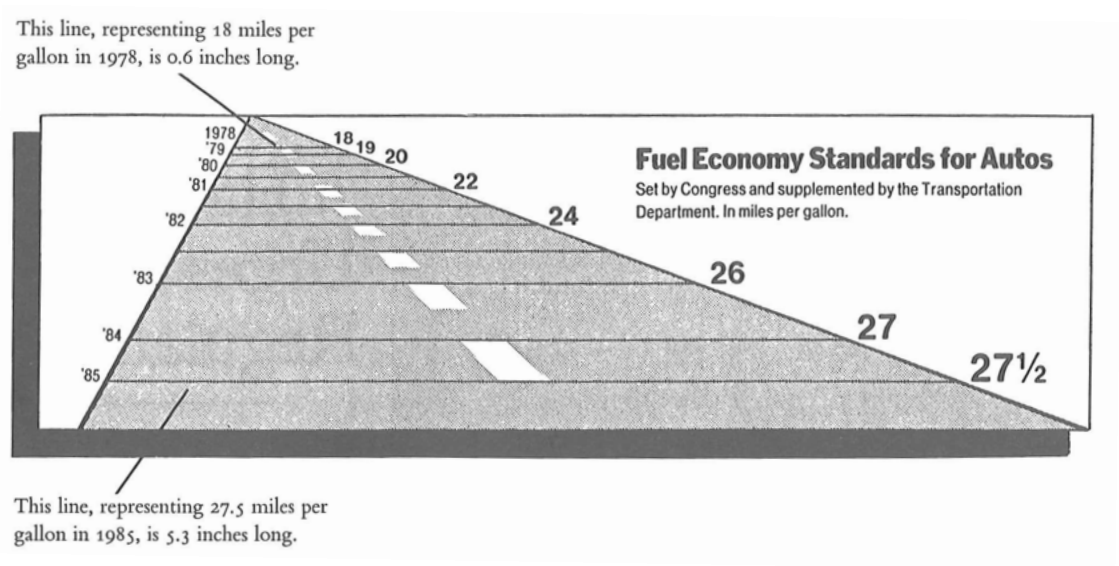
\includegraphics[keepaspectratio]{droga.png}}

{[}Tufte, 1991{]} Edward Tufte, The Visual Display of Quantitative
Information, Second Edition, Graphics Press, USA, 1991, p.~57 -- 69.

\[\operatorname{LieFactor} = \frac{\text{rozmiar efektu widocznego na wykresie}}{\text{rozmiar efektu wynikającego z danych}}\]

\[\text{rozmiar efektu} = \frac{|\text{druga wartość}-\text{pierwsza wartość}|}{\text{pierwsza wartość}}\]

\pandocbounded{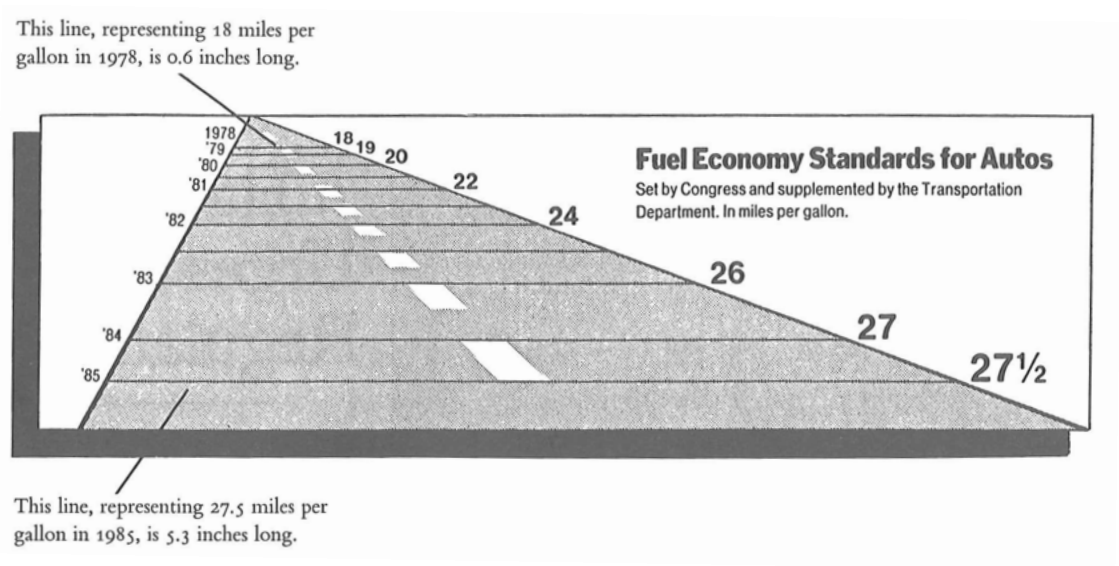
\includegraphics[keepaspectratio]{droga.png}}

\[\operatorname{LieFactor} = \frac{\frac{5.3-0.6}{0.6}}{\frac{27.5-18}{18}} \approx 14.8\]

\section{Bibliografia}\label{bibliografia-1}

\begin{itemize}
\tightlist
\item
  https://pl.wikipedia.org/wiki/Wizualizacja
\item
  https://mfiles.pl/pl/index.php/Analiza\_danych, dostęp online
  1.04.2019.
\item
  Walesiak M., Gatnar E., Statystyczna analiza danych z wykorzystaniem
  programu R, PWN, Warszawa, 2009.
\item
  Wasilewska E., Statystyka opisowa od podstaw, Podręcznik z zadaniami,
  Wydawnictwo SGGW, Warszawa, 2009.
\item
  https://en.wikipedia.org/wiki/Cognitive\_reflection\_test, dostęp
  online 20.03.2023.
\item
  https://qlikblog.pl/edward-tufte-dobre-praktyki-prezentacji-danych/,
  dostęp online 20.03.2023.
\end{itemize}

\part{NumPy}

\chapter{NumPy - start}\label{numpy---start}

NumPy jest biblioteką Pythona służącą do obliczeń naukowych.

Zastosowania:

\begin{itemize}
\tightlist
\item
  algebra liniowa
\item
  zaawansowane obliczenia matematyczne (numeryczne)
\item
  całkowania
\item
  rozwiązywanie równań
\item
  \ldots{}
\end{itemize}

\section{Instalacja pakietu NumPy - opcja łatwiejsza ``do
przeklikania''}\label{instalacja-pakietu-numpy---opcja-ux142atwiejsza-do-przeklikania}

\begin{itemize}
\tightlist
\item
  Tworzy projekt w PyCharm z venv - wersja 3.12.
\end{itemize}

\pandocbounded{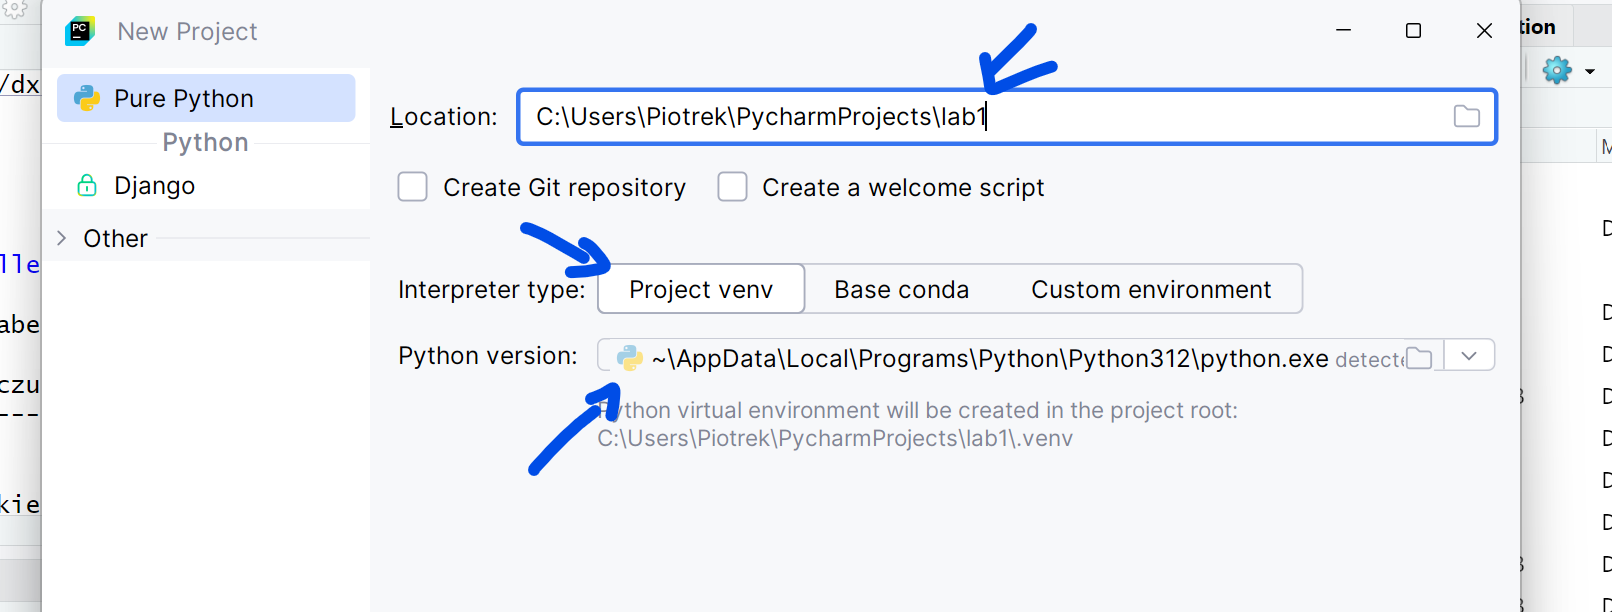
\includegraphics[keepaspectratio]{q1.png}}

\begin{itemize}
\tightlist
\item
  Za pomocą zakładki po lewej stronie na dole wyszukujemy pakiet i
  wybieramy instalację
\end{itemize}

\pandocbounded{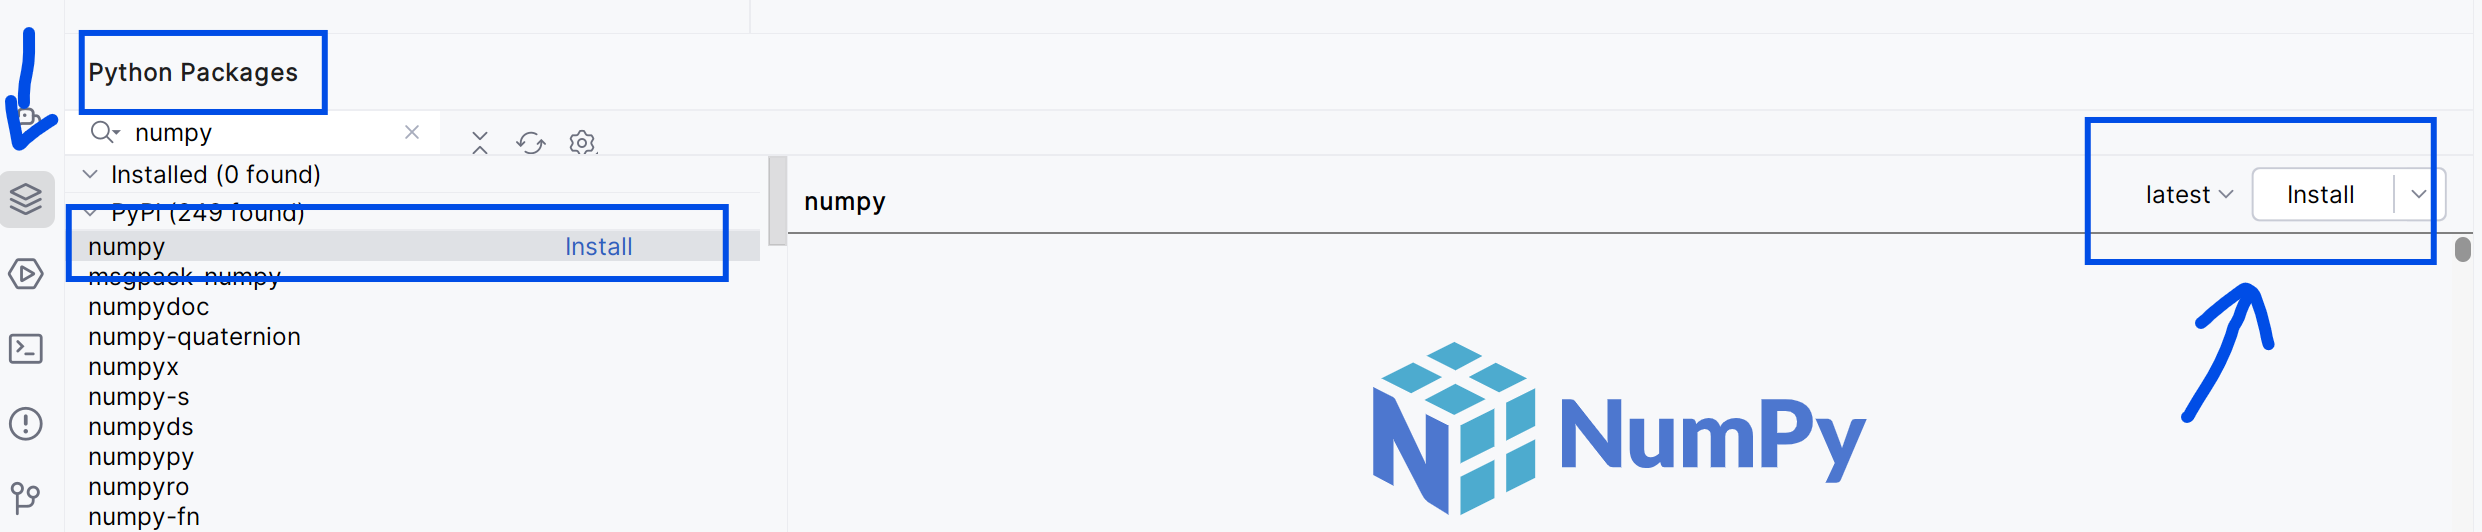
\includegraphics[keepaspectratio]{q2.png}}

\section{Instalacja pakietu NumPy - opcja
terminala}\label{instalacja-pakietu-numpy---opcja-terminala}

Komenda dla terminala:

\begin{Shaded}
\begin{Highlighting}[]
\ExtensionTok{python} \AttributeTok{{-}m}\NormalTok{ pip install numpy}
\end{Highlighting}
\end{Shaded}

\begin{Shaded}
\begin{Highlighting}[]
\ExtensionTok{python} \AttributeTok{{-}m}\NormalTok{ pip install numpy==2.2.0}
\end{Highlighting}
\end{Shaded}

\section{Import biblioteki NumPy}\label{import-biblioteki-numpy}

\begin{Shaded}
\begin{Highlighting}[]
\ImportTok{import}\NormalTok{ numpy }\ImportTok{as}\NormalTok{ np}
\end{Highlighting}
\end{Shaded}

Podstawowym bytem w bibliotece NumPy jest N-wymiarowa tablica zwana
\texttt{ndarray}. Każdy element na tablicy traktowany jest jako typ
\texttt{dtype}.

\begin{Shaded}
\begin{Highlighting}[]
\NormalTok{numpy.array(}\BuiltInTok{object}\NormalTok{, dtype}\OperatorTok{=}\VariableTok{None}\NormalTok{, }\OperatorTok{*}\NormalTok{, copy}\OperatorTok{=}\VariableTok{True}\NormalTok{, order}\OperatorTok{=}\StringTok{\textquotesingle{}K\textquotesingle{}}\NormalTok{, subok}\OperatorTok{=}\VariableTok{False}\NormalTok{, ndmin}\OperatorTok{=}\DecValTok{0}\NormalTok{, like}\OperatorTok{=}\VariableTok{None}\NormalTok{)}
\end{Highlighting}
\end{Shaded}

\begin{itemize}
\tightlist
\item
  object - to co ma być wrzucone do tablicy
\item
  dtype - typ
\item
  copy - czy obiekty mają być skopiowane, domyślne \texttt{True}
\item
  order - sposób układania: C (rzędy), F (kolumny), A, K
\item
  subok - realizowane przez podklasy (jeśli \texttt{True}), domyślnie
  \texttt{False}
\item
  ndmin - minimalny rozmiar (wymiar) tablicy
\item
  like - tworzenie na podstawie tablic referencyjnej
\end{itemize}

\phantomsection\label{annotated-cell-5}%
\begin{Shaded}
\begin{Highlighting}[]
\ImportTok{import}\NormalTok{ numpy }\ImportTok{as}\NormalTok{ np}

\NormalTok{a }\OperatorTok{=}\NormalTok{ np.array([}\DecValTok{1}\NormalTok{, }\DecValTok{2}\NormalTok{, }\DecValTok{3}\NormalTok{]) }\hspace*{\fill}\NormalTok{\circled{1}}
\BuiltInTok{print}\NormalTok{(}\StringTok{"a:"}\NormalTok{, a) }
\BuiltInTok{print}\NormalTok{(}\StringTok{"typ a:"}\NormalTok{, }\BuiltInTok{type}\NormalTok{(a)) }\hspace*{\fill}\NormalTok{\circled{2}}
\NormalTok{b }\OperatorTok{=}\NormalTok{ np.array([}\DecValTok{1}\NormalTok{, }\DecValTok{2}\NormalTok{, }\FloatTok{3.0}\NormalTok{]) }\hspace*{\fill}\NormalTok{\circled{3}}
\BuiltInTok{print}\NormalTok{(}\StringTok{"b:"}\NormalTok{, b)}
\NormalTok{c }\OperatorTok{=}\NormalTok{ np.array([[}\DecValTok{1}\NormalTok{, }\DecValTok{2}\NormalTok{], [}\DecValTok{3}\NormalTok{, }\DecValTok{4}\NormalTok{]]) }\hspace*{\fill}\NormalTok{\circled{4}}
\BuiltInTok{print}\NormalTok{(}\StringTok{"c:"}\NormalTok{, c)}
\NormalTok{d }\OperatorTok{=}\NormalTok{ np.array([}\DecValTok{1}\NormalTok{, }\DecValTok{2}\NormalTok{, }\DecValTok{3}\NormalTok{], ndmin}\OperatorTok{=}\DecValTok{2}\NormalTok{) }\hspace*{\fill}\NormalTok{\circled{5}}
\BuiltInTok{print}\NormalTok{(}\StringTok{"d:"}\NormalTok{, d)}
\NormalTok{e }\OperatorTok{=}\NormalTok{ np.array([}\DecValTok{1}\NormalTok{, }\DecValTok{2}\NormalTok{, }\DecValTok{3}\NormalTok{], dtype}\OperatorTok{=}\BuiltInTok{complex}\NormalTok{) }\hspace*{\fill}\NormalTok{\circled{6}}
\BuiltInTok{print}\NormalTok{(}\StringTok{"e:"}\NormalTok{, e)}
\NormalTok{f }\OperatorTok{=}\NormalTok{ np.array(np.asmatrix(}\StringTok{\textquotesingle{}1 2; 3 4\textquotesingle{}}\NormalTok{)) }\hspace*{\fill}\NormalTok{\circled{7}}
\BuiltInTok{print}\NormalTok{(}\StringTok{"f:"}\NormalTok{, f)}
\NormalTok{g }\OperatorTok{=}\NormalTok{ np.array(np.asmatrix(}\StringTok{\textquotesingle{}1 2; 3 4\textquotesingle{}}\NormalTok{), subok}\OperatorTok{=}\VariableTok{True}\NormalTok{) }\hspace*{\fill}\NormalTok{\circled{8}}
\BuiltInTok{print}\NormalTok{(}\StringTok{"g:"}\NormalTok{, g)}
\BuiltInTok{print}\NormalTok{(}\BuiltInTok{type}\NormalTok{(g))}
\end{Highlighting}
\end{Shaded}

\begin{description}
\tightlist
\item[\circled{1}]
Standardowe domyślne.
\item[\circled{2}]
Sprawdzenie typu.
\item[\circled{3}]
Jeden z elementów jest innego typu. Tu następuje zatem rozszerzenie do
typu ``największego''.
\item[\circled{4}]
Tu otrzymamy tablicę 2x2.
\item[\circled{5}]
W tej linijce otrzymana będzie tablica 2x1.
\item[\circled{6}]
Ustalenie innego typu - większego.
\item[\circled{7}]
Skorzystanie z podtypu macierzowego.
\item[\circled{8}]
Zachowanie typu macierzowego.
\end{description}

\begin{verbatim}
a: [1 2 3]
typ a: <class 'numpy.ndarray'>
b: [1. 2. 3.]
c: [[1 2]
 [3 4]]
d: [[1 2 3]]
e: [1.+0.j 2.+0.j 3.+0.j]
f: [[1 2]
 [3 4]]
g: [[1 2]
 [3 4]]
<class 'numpy.matrix'>
\end{verbatim}

\section{Uruchamianie - tryb ``Run''
(wykonawczy)}\label{uruchamianie---tryb-run-wykonawczy}

Run - zielona strzałka u góry.

\pandocbounded{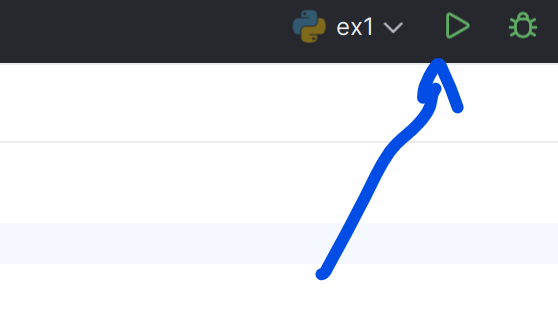
\includegraphics[keepaspectratio]{q3.png}}

\section{Uruchamianie - tryb ``Run in Python Console''
(interaktywno-wykonawczy)}\label{uruchamianie---tryb-run-in-python-console-interaktywno-wykonawczy}

\pandocbounded{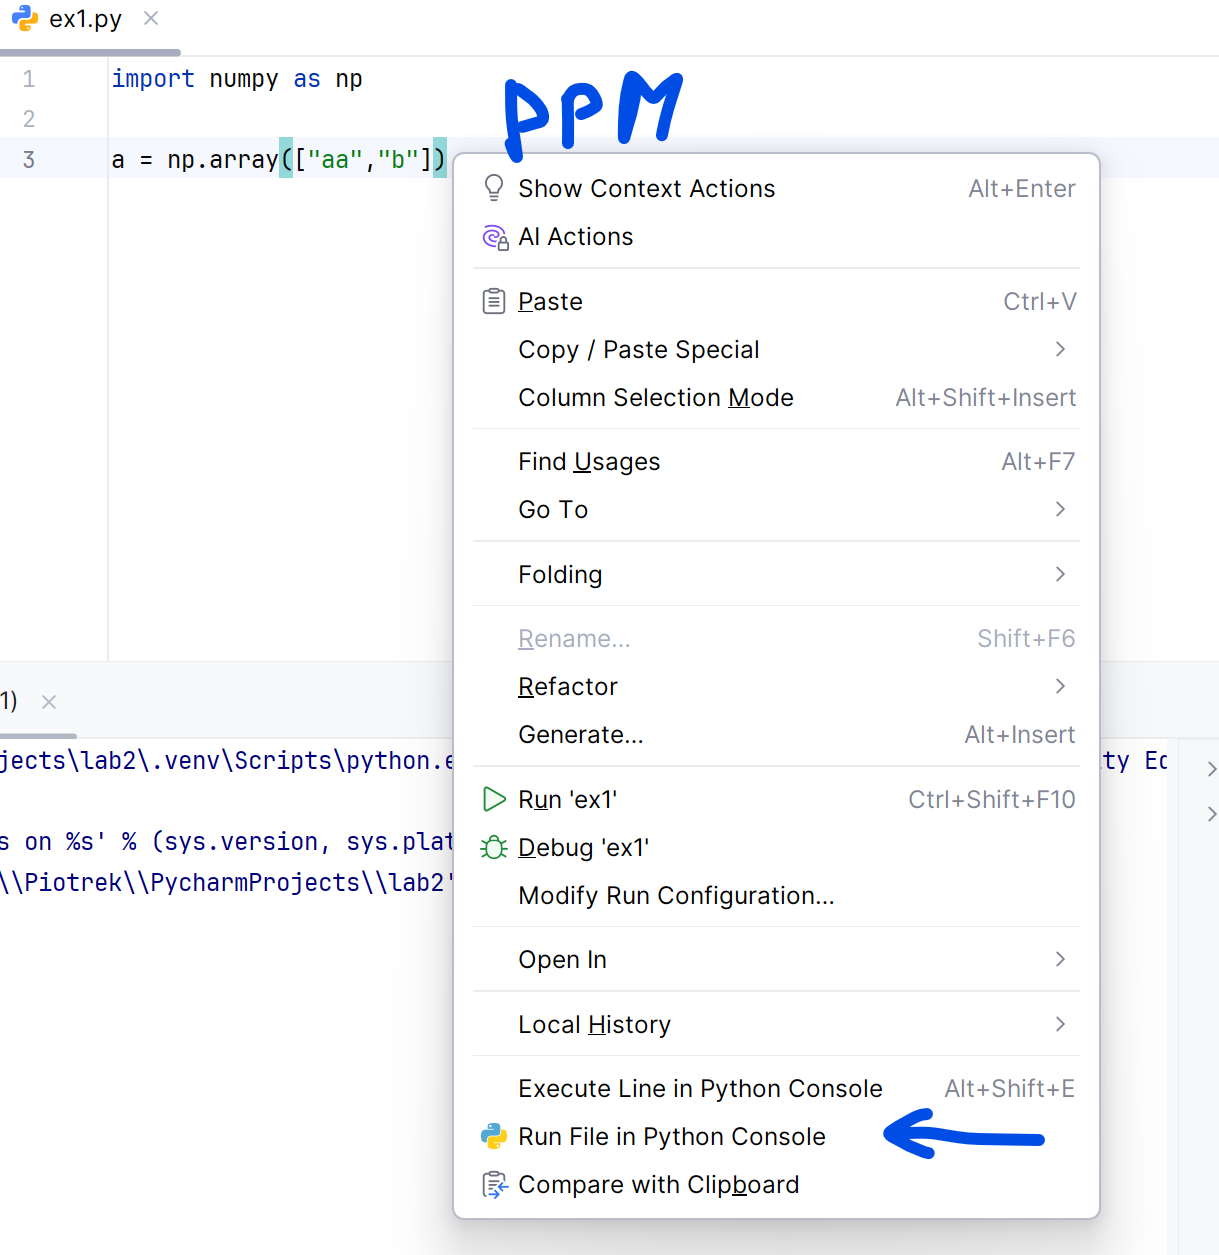
\includegraphics[keepaspectratio]{q4.png}}

\textbf{Ćwiczenie (\texttt{ex1.py}):}

\begin{enumerate}
\def\labelenumi{\arabic{enumi}.}
\tightlist
\item
  Stwórz proste tablice:
\end{enumerate}

\begin{itemize}
\item
  \(\begin{bmatrix}
  1 & 2 & 7\\
  6 & -3 & -3
  \end{bmatrix}\)
\item
  \(\begin{bmatrix}
  6 & 8 & 9 & -3
  \end{bmatrix}\)
\item
  \(\begin{bmatrix}
  4 \\ 3 \\-3 \\-7
  \end{bmatrix}\)
\item
  \(\begin{bmatrix}
  bb & cc & ww & 44
  \end{bmatrix}\)
\end{itemize}

\chapter{Lista a tablica}\label{lista-a-tablica}

\begin{Shaded}
\begin{Highlighting}[]
\ImportTok{import}\NormalTok{ numpy }\ImportTok{as}\NormalTok{ np}
\ImportTok{import}\NormalTok{ time}

\NormalTok{start\_time }\OperatorTok{=}\NormalTok{ time.time()}
\NormalTok{my\_arr }\OperatorTok{=}\NormalTok{ np.arange(}\DecValTok{1000000}\NormalTok{)}
\NormalTok{my\_list }\OperatorTok{=} \BuiltInTok{list}\NormalTok{(}\BuiltInTok{range}\NormalTok{(}\DecValTok{1000000}\NormalTok{))}
\NormalTok{start\_time }\OperatorTok{=}\NormalTok{ time.time()}
\NormalTok{my\_arr2 }\OperatorTok{=}\NormalTok{ my\_arr }\OperatorTok{*} \DecValTok{2}
\BuiltInTok{print}\NormalTok{(}\StringTok{"{-}{-}{-} }\SpecialCharTok{\%s}\StringTok{ seconds {-}{-}{-}"} \OperatorTok{\%}\NormalTok{ (time.time() }\OperatorTok{{-}}\NormalTok{ start\_time))}
\NormalTok{start\_time }\OperatorTok{=}\NormalTok{ time.time()}
\NormalTok{my\_list2 }\OperatorTok{=}\NormalTok{ [x }\OperatorTok{*} \DecValTok{2} \ControlFlowTok{for}\NormalTok{ x }\KeywordTok{in}\NormalTok{ my\_list]}
\BuiltInTok{print}\NormalTok{(}\StringTok{"{-}{-}{-} }\SpecialCharTok{\%s}\StringTok{ seconds {-}{-}{-}"} \OperatorTok{\%}\NormalTok{ (time.time() }\OperatorTok{{-}}\NormalTok{ start\_time))}
\end{Highlighting}
\end{Shaded}

\begin{verbatim}
--- 0.0016911029815673828 seconds ---
--- 0.030064105987548828 seconds ---
\end{verbatim}

\chapter{\texorpdfstring{Atrybuty tablic
\texttt{ndarray}}{Atrybuty tablic ndarray}}\label{atrybuty-tablic-ndarray}

\begin{longtable}[]{@{}
  >{\raggedright\arraybackslash}p{(\linewidth - 2\tabcolsep) * \real{0.5000}}
  >{\raggedright\arraybackslash}p{(\linewidth - 2\tabcolsep) * \real{0.5000}}@{}}
\toprule\noalign{}
\begin{minipage}[b]{\linewidth}\raggedright
Atrybut
\end{minipage} & \begin{minipage}[b]{\linewidth}\raggedright
Opis
\end{minipage} \\
\midrule\noalign{}
\endhead
\bottomrule\noalign{}
\endlastfoot
\texttt{shape} & krotka z informacją o liczbie elementów dla każdego z
wymiarów \\
\texttt{size} & liczba elementów w tablicy (łączna) \\
\texttt{ndim} & liczba wymiarów tablicy \\
\texttt{nbytes} & liczba bajtów jaką tablica zajmuje w pamięci \\
\texttt{dtype} & typ danych \\
\end{longtable}

\begin{Shaded}
\begin{Highlighting}[]
\ImportTok{import}\NormalTok{ numpy }\ImportTok{as}\NormalTok{ np}

\NormalTok{tab1 }\OperatorTok{=}\NormalTok{ np.array([}\DecValTok{2}\NormalTok{, }\OperatorTok{{-}}\DecValTok{3}\NormalTok{, }\DecValTok{4}\NormalTok{, }\OperatorTok{{-}}\DecValTok{8}\NormalTok{, }\DecValTok{1}\NormalTok{])}
\BuiltInTok{print}\NormalTok{(}\StringTok{"typ:"}\NormalTok{, }\BuiltInTok{type}\NormalTok{(tab1))}
\BuiltInTok{print}\NormalTok{(}\StringTok{"shape:"}\NormalTok{, tab1.shape)}
\BuiltInTok{print}\NormalTok{(}\StringTok{"size:"}\NormalTok{, tab1.size)}
\BuiltInTok{print}\NormalTok{(}\StringTok{"ndim:"}\NormalTok{, tab1.ndim)}
\BuiltInTok{print}\NormalTok{(}\StringTok{"nbytes:"}\NormalTok{, tab1.nbytes)}
\BuiltInTok{print}\NormalTok{(}\StringTok{"dtype:"}\NormalTok{, tab1.dtype)}
\end{Highlighting}
\end{Shaded}

\begin{verbatim}
typ: <class 'numpy.ndarray'>
shape: (5,)
size: 5
ndim: 1
nbytes: 40
dtype: int64
\end{verbatim}

\begin{Shaded}
\begin{Highlighting}[]
\ImportTok{import}\NormalTok{ numpy }\ImportTok{as}\NormalTok{ np}

\NormalTok{tab2 }\OperatorTok{=}\NormalTok{ np.array([[}\DecValTok{2}\NormalTok{, }\OperatorTok{{-}}\DecValTok{3}\NormalTok{], [}\DecValTok{4}\NormalTok{, }\OperatorTok{{-}}\DecValTok{8}\NormalTok{]])}
\BuiltInTok{print}\NormalTok{(}\StringTok{"typ:"}\NormalTok{, }\BuiltInTok{type}\NormalTok{(tab2))}
\BuiltInTok{print}\NormalTok{(}\StringTok{"shape:"}\NormalTok{, tab2.shape)}
\BuiltInTok{print}\NormalTok{(}\StringTok{"size:"}\NormalTok{, tab2.size)}
\BuiltInTok{print}\NormalTok{(}\StringTok{"ndim:"}\NormalTok{, tab2.ndim)}
\BuiltInTok{print}\NormalTok{(}\StringTok{"nbytes:"}\NormalTok{, tab2.nbytes)}
\BuiltInTok{print}\NormalTok{(}\StringTok{"dtype:"}\NormalTok{, tab2.dtype)}
\end{Highlighting}
\end{Shaded}

\begin{verbatim}
typ: <class 'numpy.ndarray'>
shape: (2, 2)
size: 4
ndim: 2
nbytes: 32
dtype: int64
\end{verbatim}

NumPy nie wspiera postrzępionych tablic! Poniższy kod wygeneruje błąd:

\begin{Shaded}
\begin{Highlighting}[]
\ImportTok{import}\NormalTok{ numpy }\ImportTok{as}\NormalTok{ np}

\NormalTok{tab3 }\OperatorTok{=}\NormalTok{ np.array([[}\DecValTok{2}\NormalTok{, }\OperatorTok{{-}}\DecValTok{3}\NormalTok{], [}\DecValTok{4}\NormalTok{, }\OperatorTok{{-}}\DecValTok{8}\NormalTok{, }\DecValTok{5}\NormalTok{], [}\DecValTok{3}\NormalTok{]])}
\end{Highlighting}
\end{Shaded}

\textbf{Ćwiczenia:} (\texttt{ex2.py})\\
Utwórz tablice numpy: \[
A = \begin{bmatrix} 1 & 2 & 3 \\ 4 & 5 & 6 \end{bmatrix}
\] \[B = \begin{bmatrix} 7 & 8 \\ 9 & 10 \\ 11 & 12 \end{bmatrix}\]
\[C = \begin{bmatrix} 1.1 & 2.2 & 3.3 \\ 4.4 & 5.5 & 6.6 \end{bmatrix}\]
i sprawdź ich parametry.

\chapter{Typy danych}\label{typy-danych}

\begin{longtable}[]{@{}
  >{\raggedright\arraybackslash}p{(\linewidth - 2\tabcolsep) * \real{0.5000}}
  >{\raggedright\arraybackslash}p{(\linewidth - 2\tabcolsep) * \real{0.5000}}@{}}
\toprule\noalign{}
\endhead
\bottomrule\noalign{}
\endlastfoot
Typy całkowitoliczbowe &
\texttt{int},\texttt{int8},\texttt{int16},\texttt{int32},\texttt{int64} \\
Typy całkowitoliczbowe (bez znaku) &
\texttt{uint},\texttt{uint8},\texttt{uint16},\texttt{uint32},\texttt{uint64} \\
Typ logiczny & \texttt{bool} \\
Typy zmiennoprzecinkowe & \texttt{float}, \texttt{float16},
\texttt{float32}, \texttt{float64}, \texttt{float128} \\
Typy zmiennoprzecinkowe zespolone & \texttt{complex},
\texttt{complex64}, \texttt{complex128}, \texttt{complex256} \\
Napis & \texttt{str} \\
\end{longtable}

\begin{Shaded}
\begin{Highlighting}[]
\ImportTok{import}\NormalTok{ numpy }\ImportTok{as}\NormalTok{ np}

\NormalTok{tab }\OperatorTok{=}\NormalTok{ np.array([[}\DecValTok{2}\NormalTok{, }\OperatorTok{{-}}\DecValTok{3}\NormalTok{], [}\DecValTok{4}\NormalTok{, }\OperatorTok{{-}}\DecValTok{8}\NormalTok{]])}
\BuiltInTok{print}\NormalTok{(tab)}
\NormalTok{tab2 }\OperatorTok{=}\NormalTok{ np.array([[}\DecValTok{2}\NormalTok{, }\OperatorTok{{-}}\DecValTok{3}\NormalTok{], [}\DecValTok{4}\NormalTok{, }\OperatorTok{{-}}\DecValTok{8}\NormalTok{]], dtype}\OperatorTok{=}\BuiltInTok{int}\NormalTok{)}
\BuiltInTok{print}\NormalTok{(tab2)}
\NormalTok{tab3 }\OperatorTok{=}\NormalTok{ np.array([[}\DecValTok{2}\NormalTok{, }\OperatorTok{{-}}\DecValTok{3}\NormalTok{], [}\DecValTok{4}\NormalTok{, }\OperatorTok{{-}}\DecValTok{8}\NormalTok{]], dtype}\OperatorTok{=}\BuiltInTok{float}\NormalTok{)}
\BuiltInTok{print}\NormalTok{(tab3)}
\NormalTok{tab4 }\OperatorTok{=}\NormalTok{ np.array([[}\DecValTok{2}\NormalTok{, }\OperatorTok{{-}}\DecValTok{3}\NormalTok{], [}\DecValTok{4}\NormalTok{, }\OperatorTok{{-}}\DecValTok{8}\NormalTok{]], dtype}\OperatorTok{=}\BuiltInTok{complex}\NormalTok{)}
\BuiltInTok{print}\NormalTok{(tab4)}
\end{Highlighting}
\end{Shaded}

\begin{verbatim}
[[ 2 -3]
 [ 4 -8]]
[[ 2 -3]
 [ 4 -8]]
[[ 2. -3.]
 [ 4. -8.]]
[[ 2.+0.j -3.+0.j]
 [ 4.+0.j -8.+0.j]]
\end{verbatim}

\chapter{Tworzenie tablic}\label{tworzenie-tablic}

\texttt{np.array} - argumenty rzutowany na tablicę (coś po czym można
iterować) - warto sprawdzić rozmiar/kształt

\begin{Shaded}
\begin{Highlighting}[]
\ImportTok{import}\NormalTok{ numpy }\ImportTok{as}\NormalTok{ np}

\NormalTok{tab }\OperatorTok{=}\NormalTok{ np.array([}\DecValTok{2}\NormalTok{, }\OperatorTok{{-}}\DecValTok{3}\NormalTok{, }\DecValTok{4}\NormalTok{])}
\BuiltInTok{print}\NormalTok{(tab)}
\BuiltInTok{print}\NormalTok{(}\StringTok{"size:"}\NormalTok{, tab.size)}
\NormalTok{tab2 }\OperatorTok{=}\NormalTok{ np.array((}\DecValTok{4}\NormalTok{, }\OperatorTok{{-}}\DecValTok{3}\NormalTok{, }\DecValTok{3}\NormalTok{, }\DecValTok{2}\NormalTok{))}
\BuiltInTok{print}\NormalTok{(tab2)}
\BuiltInTok{print}\NormalTok{(}\StringTok{"size:"}\NormalTok{, tab2.size)}
\NormalTok{tab3 }\OperatorTok{=}\NormalTok{ np.array(\{}\DecValTok{3}\NormalTok{, }\DecValTok{3}\NormalTok{, }\DecValTok{2}\NormalTok{, }\DecValTok{5}\NormalTok{, }\DecValTok{2}\NormalTok{\})}
\BuiltInTok{print}\NormalTok{(tab3)}
\BuiltInTok{print}\NormalTok{(}\StringTok{"size:"}\NormalTok{, tab3.size)}
\NormalTok{tab4 }\OperatorTok{=}\NormalTok{ np.array(\{}\StringTok{"pl"}\NormalTok{: }\DecValTok{344}\NormalTok{, }\StringTok{"en"}\NormalTok{: }\DecValTok{22}\NormalTok{\})}
\BuiltInTok{print}\NormalTok{(tab4)}
\BuiltInTok{print}\NormalTok{(}\StringTok{"size:"}\NormalTok{, tab4.size)}
\end{Highlighting}
\end{Shaded}

\begin{verbatim}
[ 2 -3  4]
size: 3
[ 4 -3  3  2]
size: 4
{2, 3, 5}
size: 1
{'pl': 344, 'en': 22}
size: 1
\end{verbatim}

\texttt{np.zeros} - tworzy tablicę wypełnioną zerami

\begin{Shaded}
\begin{Highlighting}[]
\ImportTok{import}\NormalTok{ numpy }\ImportTok{as}\NormalTok{ np}

\NormalTok{tab }\OperatorTok{=}\NormalTok{ np.zeros(}\DecValTok{4}\NormalTok{)}
\BuiltInTok{print}\NormalTok{(tab)}
\BuiltInTok{print}\NormalTok{(tab.shape)}
\NormalTok{tab2 }\OperatorTok{=}\NormalTok{ np.zeros([}\DecValTok{2}\NormalTok{, }\DecValTok{3}\NormalTok{])}
\BuiltInTok{print}\NormalTok{(tab2)}
\BuiltInTok{print}\NormalTok{(tab2.shape)}
\NormalTok{tab3 }\OperatorTok{=}\NormalTok{ np.zeros([}\DecValTok{2}\NormalTok{, }\DecValTok{3}\NormalTok{, }\DecValTok{4}\NormalTok{])}
\BuiltInTok{print}\NormalTok{(tab3)}
\BuiltInTok{print}\NormalTok{(tab3.shape)}
\end{Highlighting}
\end{Shaded}

\begin{verbatim}
[0. 0. 0. 0.]
(4,)
[[0. 0. 0.]
 [0. 0. 0.]]
(2, 3)
[[[0. 0. 0. 0.]
  [0. 0. 0. 0.]
  [0. 0. 0. 0.]]

 [[0. 0. 0. 0.]
  [0. 0. 0. 0.]
  [0. 0. 0. 0.]]]
(2, 3, 4)
\end{verbatim}

\texttt{np.ones} - tworzy tablicę wypełnioną jedynkami (to nie
odpowiednik macierzy jednostkowej!)

\begin{Shaded}
\begin{Highlighting}[]
\ImportTok{import}\NormalTok{ numpy }\ImportTok{as}\NormalTok{ np}

\NormalTok{tab }\OperatorTok{=}\NormalTok{ np.ones(}\DecValTok{4}\NormalTok{)}
\BuiltInTok{print}\NormalTok{(tab)}
\BuiltInTok{print}\NormalTok{(tab.shape)}
\NormalTok{tab2 }\OperatorTok{=}\NormalTok{ np.ones([}\DecValTok{2}\NormalTok{, }\DecValTok{3}\NormalTok{])}
\BuiltInTok{print}\NormalTok{(tab2)}
\BuiltInTok{print}\NormalTok{(tab2.shape)}
\NormalTok{tab3 }\OperatorTok{=}\NormalTok{ np.ones([}\DecValTok{2}\NormalTok{, }\DecValTok{3}\NormalTok{, }\DecValTok{4}\NormalTok{])}
\BuiltInTok{print}\NormalTok{(tab3)}
\BuiltInTok{print}\NormalTok{(tab3.shape)}
\end{Highlighting}
\end{Shaded}

\begin{verbatim}
[1. 1. 1. 1.]
(4,)
[[1. 1. 1.]
 [1. 1. 1.]]
(2, 3)
[[[1. 1. 1. 1.]
  [1. 1. 1. 1.]
  [1. 1. 1. 1.]]

 [[1. 1. 1. 1.]
  [1. 1. 1. 1.]
  [1. 1. 1. 1.]]]
(2, 3, 4)
\end{verbatim}

\texttt{np.diag} - tworzy tablicę odpowiadającą macierzy diagonalnej

\begin{Shaded}
\begin{Highlighting}[]
\ImportTok{import}\NormalTok{ numpy }\ImportTok{as}\NormalTok{ np}

\BuiltInTok{print}\NormalTok{(}\StringTok{"tab0"}\NormalTok{)}
\NormalTok{tab0 }\OperatorTok{=}\NormalTok{ np.diag([}\DecValTok{3}\NormalTok{, }\DecValTok{4}\NormalTok{, }\DecValTok{5}\NormalTok{])}
\BuiltInTok{print}\NormalTok{(tab0)}
\BuiltInTok{print}\NormalTok{(}\StringTok{"tab1"}\NormalTok{)}
\NormalTok{tab1 }\OperatorTok{=}\NormalTok{ np.array([[}\DecValTok{2}\NormalTok{, }\DecValTok{3}\NormalTok{, }\DecValTok{4}\NormalTok{], [}\DecValTok{3}\NormalTok{, }\OperatorTok{{-}}\DecValTok{4}\NormalTok{, }\DecValTok{5}\NormalTok{], [}\DecValTok{3}\NormalTok{, }\DecValTok{4}\NormalTok{, }\OperatorTok{{-}}\DecValTok{5}\NormalTok{]])}
\BuiltInTok{print}\NormalTok{(tab1)}
\NormalTok{tab2 }\OperatorTok{=}\NormalTok{ np.diag(tab1)}
\BuiltInTok{print}\NormalTok{(}\StringTok{"tab2"}\NormalTok{)}
\BuiltInTok{print}\NormalTok{(tab2)}
\NormalTok{tab3 }\OperatorTok{=}\NormalTok{ np.diag(tab1, k}\OperatorTok{=}\DecValTok{1}\NormalTok{)}
\BuiltInTok{print}\NormalTok{(}\StringTok{"tab3"}\NormalTok{)}
\BuiltInTok{print}\NormalTok{(tab3)}
\BuiltInTok{print}\NormalTok{(}\StringTok{"tab4"}\NormalTok{)}
\NormalTok{tab4 }\OperatorTok{=}\NormalTok{ np.diag(tab1, k}\OperatorTok{={-}}\DecValTok{2}\NormalTok{)}
\BuiltInTok{print}\NormalTok{(tab4)}
\BuiltInTok{print}\NormalTok{(}\StringTok{"tab5"}\NormalTok{)}
\NormalTok{tab5 }\OperatorTok{=}\NormalTok{ np.diag(np.diag(tab1))}
\BuiltInTok{print}\NormalTok{(tab5)}
\end{Highlighting}
\end{Shaded}

\begin{verbatim}
tab0
[[3 0 0]
 [0 4 0]
 [0 0 5]]
tab1
[[ 2  3  4]
 [ 3 -4  5]
 [ 3  4 -5]]
tab2
[ 2 -4 -5]
tab3
[3 5]
tab4
[3]
tab5
[[ 2  0  0]
 [ 0 -4  0]
 [ 0  0 -5]]
\end{verbatim}

\texttt{np.arange} - tablica wypełniona równomiernymi wartościami

Składnia:
\texttt{numpy.arange({[}start,\ {]}stop,\ {[}step,\ {]}dtype=None)}

Zasada działania jest podobna jak w funkcji \texttt{range}, ale
dopuszczamy liczby ``z ułamkiem''.

\begin{Shaded}
\begin{Highlighting}[]
\ImportTok{import}\NormalTok{ numpy }\ImportTok{as}\NormalTok{ np}

\NormalTok{a }\OperatorTok{=}\NormalTok{ np.arange(}\DecValTok{3}\NormalTok{)}
\BuiltInTok{print}\NormalTok{(a)}
\NormalTok{b }\OperatorTok{=}\NormalTok{ np.arange(}\FloatTok{3.0}\NormalTok{)}
\BuiltInTok{print}\NormalTok{(b)}
\NormalTok{c }\OperatorTok{=}\NormalTok{ np.arange(}\DecValTok{3}\NormalTok{, }\DecValTok{7}\NormalTok{)}
\BuiltInTok{print}\NormalTok{(c)}
\NormalTok{d }\OperatorTok{=}\NormalTok{ np.arange(}\DecValTok{3}\NormalTok{, }\DecValTok{11}\NormalTok{, }\DecValTok{2}\NormalTok{)}
\BuiltInTok{print}\NormalTok{(d)}
\NormalTok{e }\OperatorTok{=}\NormalTok{ np.arange(}\DecValTok{0}\NormalTok{, }\DecValTok{1}\NormalTok{, }\FloatTok{0.1}\NormalTok{)}
\BuiltInTok{print}\NormalTok{(e)}
\NormalTok{f }\OperatorTok{=}\NormalTok{ np.arange(}\DecValTok{3}\NormalTok{, }\DecValTok{11}\NormalTok{, }\DecValTok{2}\NormalTok{, dtype}\OperatorTok{=}\BuiltInTok{float}\NormalTok{)}
\BuiltInTok{print}\NormalTok{(f)}
\NormalTok{g }\OperatorTok{=}\NormalTok{ np.arange(}\DecValTok{3}\NormalTok{, }\DecValTok{10}\NormalTok{, }\DecValTok{2}\NormalTok{)}
\BuiltInTok{print}\NormalTok{(g)}
\end{Highlighting}
\end{Shaded}

\begin{verbatim}
[0 1 2]
[0. 1. 2.]
[3 4 5 6]
[3 5 7 9]
[0.  0.1 0.2 0.3 0.4 0.5 0.6 0.7 0.8 0.9]
[3. 5. 7. 9.]
[3 5 7 9]
\end{verbatim}

\texttt{np.linspace} - tablica wypełniona równomiernymi wartościami wg
skali liniowej

\begin{Shaded}
\begin{Highlighting}[]
\ImportTok{import}\NormalTok{ numpy }\ImportTok{as}\NormalTok{ np}

\NormalTok{a }\OperatorTok{=}\NormalTok{ np.linspace(}\FloatTok{2.0}\NormalTok{, }\FloatTok{3.0}\NormalTok{, num}\OperatorTok{=}\DecValTok{5}\NormalTok{)}
\BuiltInTok{print}\NormalTok{(a)}
\NormalTok{b }\OperatorTok{=}\NormalTok{ np.linspace(}\FloatTok{2.0}\NormalTok{, }\FloatTok{3.0}\NormalTok{, num}\OperatorTok{=}\DecValTok{5}\NormalTok{, endpoint}\OperatorTok{=}\VariableTok{False}\NormalTok{)}
\BuiltInTok{print}\NormalTok{(b)}
\NormalTok{c }\OperatorTok{=}\NormalTok{ np.linspace(}\DecValTok{10}\NormalTok{, }\DecValTok{20}\NormalTok{, num}\OperatorTok{=}\DecValTok{4}\NormalTok{)}
\BuiltInTok{print}\NormalTok{(c)}
\NormalTok{d }\OperatorTok{=}\NormalTok{ np.linspace(}\DecValTok{10}\NormalTok{, }\DecValTok{20}\NormalTok{, num}\OperatorTok{=}\DecValTok{4}\NormalTok{, dtype}\OperatorTok{=}\BuiltInTok{int}\NormalTok{)}
\BuiltInTok{print}\NormalTok{(d)}
\end{Highlighting}
\end{Shaded}

\begin{verbatim}
[2.   2.25 2.5  2.75 3.  ]
[2.  2.2 2.4 2.6 2.8]
[10.         13.33333333 16.66666667 20.        ]
[10 13 16 20]
\end{verbatim}

\pandocbounded{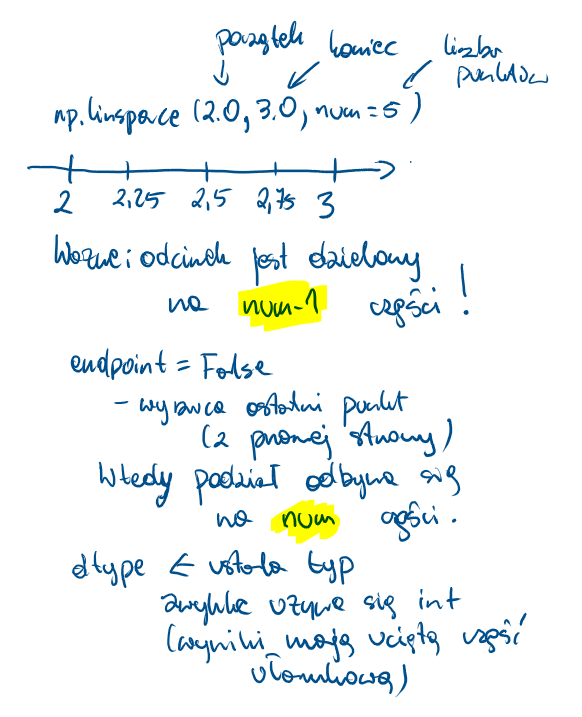
\includegraphics[keepaspectratio]{o1.png}}

\texttt{np.logspace} - tablica wypełniona wartościami wg skali
logarytmicznej

Składnia:
\texttt{numpy.logspace(start,\ stop,\ num=50,\ endpoint=True,\ base=10.0,\ dtype=None,\ axis=0)}

\begin{Shaded}
\begin{Highlighting}[]
\ImportTok{import}\NormalTok{ numpy }\ImportTok{as}\NormalTok{ np}

\NormalTok{a }\OperatorTok{=}\NormalTok{ np.logspace(}\FloatTok{2.0}\NormalTok{, }\FloatTok{3.0}\NormalTok{, num}\OperatorTok{=}\DecValTok{4}\NormalTok{)}
\BuiltInTok{print}\NormalTok{(a)}
\NormalTok{b }\OperatorTok{=}\NormalTok{ np.logspace(}\FloatTok{2.0}\NormalTok{, }\FloatTok{3.0}\NormalTok{, num}\OperatorTok{=}\DecValTok{4}\NormalTok{, endpoint}\OperatorTok{=}\VariableTok{False}\NormalTok{)}
\BuiltInTok{print}\NormalTok{(b)}
\NormalTok{c }\OperatorTok{=}\NormalTok{ np.logspace(}\FloatTok{2.0}\NormalTok{, }\FloatTok{3.0}\NormalTok{, num}\OperatorTok{=}\DecValTok{4}\NormalTok{, base}\OperatorTok{=}\FloatTok{2.0}\NormalTok{)}
\BuiltInTok{print}\NormalTok{(c)}
\end{Highlighting}
\end{Shaded}

\begin{verbatim}
[ 100.          215.443469    464.15888336 1000.        ]
[100.         177.827941   316.22776602 562.34132519]
[4.         5.0396842  6.34960421 8.        ]
\end{verbatim}

\pandocbounded{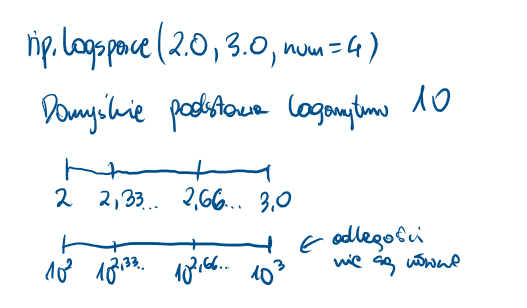
\includegraphics[keepaspectratio]{o2.png}}

\texttt{np.empty} - pusta (niezaincjowana) tablica - konkretne wartości
nie są ``gwarantowane''

\begin{Shaded}
\begin{Highlighting}[]
\ImportTok{import}\NormalTok{ numpy }\ImportTok{as}\NormalTok{ np}

\NormalTok{a }\OperatorTok{=}\NormalTok{ np.empty(}\DecValTok{3}\NormalTok{)}
\BuiltInTok{print}\NormalTok{(a)}
\NormalTok{b }\OperatorTok{=}\NormalTok{ np.empty(}\DecValTok{3}\NormalTok{, dtype}\OperatorTok{=}\BuiltInTok{int}\NormalTok{)}
\BuiltInTok{print}\NormalTok{(b)}
\end{Highlighting}
\end{Shaded}

\begin{verbatim}
[0. 1. 2.]
[                  0 4607182418800017408 4611686018427387904]
\end{verbatim}

\texttt{np.identity} - tablica przypominająca macierz jednostkową

\texttt{np.eye} - tablica z jedynkami na przekątnej (pozostałe zera)

\begin{Shaded}
\begin{Highlighting}[]
\ImportTok{import}\NormalTok{ numpy }\ImportTok{as}\NormalTok{ np}

\BuiltInTok{print}\NormalTok{(}\StringTok{"a"}\NormalTok{)}
\NormalTok{a }\OperatorTok{=}\NormalTok{ np.identity(}\DecValTok{4}\NormalTok{)}
\BuiltInTok{print}\NormalTok{(a)}
\BuiltInTok{print}\NormalTok{(}\StringTok{"b"}\NormalTok{)}
\NormalTok{b }\OperatorTok{=}\NormalTok{ np.eye(}\DecValTok{4}\NormalTok{, k}\OperatorTok{=}\DecValTok{1}\NormalTok{)}
\BuiltInTok{print}\NormalTok{(b)}
\BuiltInTok{print}\NormalTok{(}\StringTok{"c"}\NormalTok{)}
\NormalTok{c }\OperatorTok{=}\NormalTok{ np.eye(}\DecValTok{4}\NormalTok{, k}\OperatorTok{=}\DecValTok{2}\NormalTok{)}
\BuiltInTok{print}\NormalTok{(c)}
\BuiltInTok{print}\NormalTok{(}\StringTok{"d"}\NormalTok{)}
\NormalTok{d }\OperatorTok{=}\NormalTok{ np.eye(}\DecValTok{4}\NormalTok{, k}\OperatorTok{={-}}\DecValTok{1}\NormalTok{)}
\BuiltInTok{print}\NormalTok{(d)}
\end{Highlighting}
\end{Shaded}

\begin{verbatim}
a
[[1. 0. 0. 0.]
 [0. 1. 0. 0.]
 [0. 0. 1. 0.]
 [0. 0. 0. 1.]]
b
[[0. 1. 0. 0.]
 [0. 0. 1. 0.]
 [0. 0. 0. 1.]
 [0. 0. 0. 0.]]
c
[[0. 0. 1. 0.]
 [0. 0. 0. 1.]
 [0. 0. 0. 0.]
 [0. 0. 0. 0.]]
d
[[0. 0. 0. 0.]
 [1. 0. 0. 0.]
 [0. 1. 0. 0.]
 [0. 0. 1. 0.]]
\end{verbatim}

\textbf{Ćwiczenia:} (\texttt{ex3.py})

\begin{enumerate}
\def\labelenumi{\arabic{enumi}.}
\item
  Utwórz jednowymiarową tablicę zawierającą liczby całkowite od 1 do 5 i
  przypisz ją do zmiennej \texttt{A}. Wynikowa tablica powinna mieć
  postać: \[\begin{bmatrix}1 & 2 & 3 & 4 & 5\end{bmatrix} \]
\item
  Utwórz dwuwymiarową tablicę zawierającą elementy:
  \[\begin{bmatrix}1 & 2 \\ 3 & 4\end{bmatrix} \]\\
  i przypisz ją do zmiennej \texttt{B}.
\item
  Utwórz tablicę zawierającą liczby od 0 do 9 (włącznie). Przypisz ją do
  zmiennej \texttt{C}.\\
  Oczekiwana postać:
  \[\begin{bmatrix}0 & 1 & 2 & 3 & 4 & 5 & 6 & 7 & 8 & 9\end{bmatrix} \]
\item
  Utwórz tablicę zawierającą liczby od 10 do 30 z krokiem 5. Przypisz do
  \texttt{D}.\\
  Oczekiwana postać:
  \[\begin{bmatrix}10 & 15 & 20 & 25 & 30\end{bmatrix} \]
\item
  Utwórz tablicę 5 wartości równomiernie rozłożonych pomiędzy 0 a 1.
  Przypisz do \texttt{E}.\\
  Przykładowa postać:
  \[\begin{bmatrix}0. & 0.25 & 0.5 & 0.75 & 1.\end{bmatrix} \]
\item
  Utwórz dwuwymiarową tablicę o wymiarach 2x3 wypełnioną zerami.
  Przypisz do \texttt{F}.\\
  Oczekiwana postać:
  \[\begin{bmatrix}0 & 0 & 0 \\ 0 & 0 & 0\end{bmatrix} \]
\item
  Korzystając z \texttt{np.eye} utwórz macierz jednostkową 4x4. Przypisz
  do \texttt{J}.\\
  Oczekiwana postać:
  \[\begin{bmatrix}1 & 0 & 0 & 0 \\ 0 & 1 & 0 & 0 \\ 0 & 0 & 1 & 0 \\ 0 & 0 & 0 & 1\end{bmatrix} \]
\end{enumerate}

\chapter{Indeksowanie, ``krojenie''}\label{indeksowanie-krojenie}

\phantomsection\label{annotated-cell-20}%
\begin{Shaded}
\begin{Highlighting}[]
\ImportTok{import}\NormalTok{ numpy }\ImportTok{as}\NormalTok{ np}

\NormalTok{a }\OperatorTok{=}\NormalTok{ np.array([}\DecValTok{2}\NormalTok{, }\DecValTok{5}\NormalTok{, }\OperatorTok{{-}}\DecValTok{2}\NormalTok{, }\DecValTok{4}\NormalTok{, }\OperatorTok{{-}}\DecValTok{7}\NormalTok{, }\DecValTok{8}\NormalTok{, }\DecValTok{9}\NormalTok{, }\DecValTok{11}\NormalTok{, }\OperatorTok{{-}}\DecValTok{23}\NormalTok{, }\OperatorTok{{-}}\DecValTok{4}\NormalTok{, }\OperatorTok{{-}}\DecValTok{7}\NormalTok{, }\DecValTok{16}\NormalTok{, }\DecValTok{1}\NormalTok{])}
\BuiltInTok{print}\NormalTok{(}\StringTok{"1:"}\NormalTok{, a[}\DecValTok{5}\NormalTok{]) }\hspace*{\fill}\NormalTok{\circled{1}}
\BuiltInTok{print}\NormalTok{(}\StringTok{"2:"}\NormalTok{, a[}\OperatorTok{{-}}\DecValTok{2}\NormalTok{]) }\hspace*{\fill}\NormalTok{\circled{2}}
\BuiltInTok{print}\NormalTok{(}\StringTok{"3:"}\NormalTok{, a[}\DecValTok{3}\NormalTok{:}\DecValTok{6}\NormalTok{]) }\hspace*{\fill}\NormalTok{\circled{3}}
\BuiltInTok{print}\NormalTok{(}\StringTok{"4:"}\NormalTok{, a[:]) }\hspace*{\fill}\NormalTok{\circled{4}}
\BuiltInTok{print}\NormalTok{(}\StringTok{"5:"}\NormalTok{, a[}\DecValTok{0}\NormalTok{:}\OperatorTok{{-}}\DecValTok{1}\NormalTok{]) }\hspace*{\fill}\NormalTok{\circled{5}}
\BuiltInTok{print}\NormalTok{(}\StringTok{"6:"}\NormalTok{, a[:}\DecValTok{5}\NormalTok{]) }\hspace*{\fill}\NormalTok{\circled{6}}
\end{Highlighting}
\end{Shaded}

\begin{description}
\tightlist
\item[\circled{1}]
Dostęp do elementu o indeksie 5.
\item[\circled{2}]
Dostęp do elementu drugiego od tyłu.
\item[\circled{3}]
Dostęp do elementów o indeksach od 3 do 5 (włącznie) - zasada
przedziałów lewostronnnie domkniętnych, prawostronnie otwartych.
\item[\circled{4}]
Dostęp do wszystkich elementów.
\item[\circled{5}]
Dostęp do wszystkich elementów z wyłączeniem ostatniego.
\item[\circled{6}]
Dostęp od początku do elementu o indeksie 4.
\end{description}

\begin{verbatim}
1: 8
2: 16
3: [ 4 -7  8]
4: [  2   5  -2   4  -7   8   9  11 -23  -4  -7  16   1]
5: [  2   5  -2   4  -7   8   9  11 -23  -4  -7  16]
6: [ 2  5 -2  4 -7]
\end{verbatim}

\phantomsection\label{annotated-cell-21}%
\begin{Shaded}
\begin{Highlighting}[]
\ImportTok{import}\NormalTok{ numpy }\ImportTok{as}\NormalTok{ np}

\BuiltInTok{print}\NormalTok{(}\StringTok{"1:"}\NormalTok{, a[}\DecValTok{4}\NormalTok{:]) }\hspace*{\fill}\NormalTok{\circled{1}}
\BuiltInTok{print}\NormalTok{(}\StringTok{"2:"}\NormalTok{, a[}\DecValTok{4}\NormalTok{:}\OperatorTok{{-}}\DecValTok{1}\NormalTok{]) }\hspace*{\fill}\NormalTok{\circled{2}}
\BuiltInTok{print}\NormalTok{(}\StringTok{"3:"}\NormalTok{, a[}\DecValTok{4}\NormalTok{:}\DecValTok{10}\NormalTok{:}\DecValTok{2}\NormalTok{]) }\hspace*{\fill}\NormalTok{\circled{3}}
\BuiltInTok{print}\NormalTok{(}\StringTok{"4:"}\NormalTok{, a[::}\OperatorTok{{-}}\DecValTok{1}\NormalTok{]) }\hspace*{\fill}\NormalTok{\circled{4}}
\BuiltInTok{print}\NormalTok{(}\StringTok{"5:"}\NormalTok{, a[::}\DecValTok{2}\NormalTok{]) }\hspace*{\fill}\NormalTok{\circled{5}}
\BuiltInTok{print}\NormalTok{(}\StringTok{"6:"}\NormalTok{, a[::}\OperatorTok{{-}}\DecValTok{2}\NormalTok{]) }\hspace*{\fill}\NormalTok{\circled{6}}
\end{Highlighting}
\end{Shaded}

\begin{description}
\tightlist
\item[\circled{1}]
Dostęp do elementów od indeksu 4 do końca.
\item[\circled{2}]
Dostęp do elementów od indeksu 4 do końca bez ostatniego.
\item[\circled{3}]
Dostęp do elementów o indeksach stanowiących ciąg arytmetyczny od 4 do
10 (z czówrką, ale bez dziesiątki) z krokiem równym 2
\item[\circled{4}]
Dostęp do elementów od tyłu do początku.
\item[\circled{5}]
Dostęp do elementów o indeksach parzystych od początku.
\item[\circled{6}]
Dostęp do elementów o indeksach ``nieparzystych ujemnych'' od początku.
\end{description}

\begin{verbatim}
1: [ -7   8   9  11 -23  -4  -7  16   1]
2: [ -7   8   9  11 -23  -4  -7  16]
3: [ -7   9 -23]
4: [  1  16  -7  -4 -23  11   9   8  -7   4  -2   5   2]
5: [  2  -2  -7   9 -23  -7   1]
6: [  1  -7 -23   9  -7  -2   2]
\end{verbatim}

\begin{Shaded}
\begin{Highlighting}[]
\ImportTok{import}\NormalTok{ numpy }\ImportTok{as}\NormalTok{ np}

\NormalTok{a }\OperatorTok{=}\NormalTok{ np.array([[}\DecValTok{3}\NormalTok{, }\DecValTok{4}\NormalTok{, }\DecValTok{5}\NormalTok{], [}\OperatorTok{{-}}\DecValTok{3}\NormalTok{, }\DecValTok{4}\NormalTok{, }\DecValTok{8}\NormalTok{], [}\DecValTok{3}\NormalTok{, }\DecValTok{2}\NormalTok{, }\DecValTok{9}\NormalTok{]])}
\NormalTok{b }\OperatorTok{=}\NormalTok{ a[:}\DecValTok{2}\NormalTok{, }\DecValTok{1}\NormalTok{:]}
\BuiltInTok{print}\NormalTok{(b)}
\BuiltInTok{print}\NormalTok{(np.shape(b))}
\NormalTok{c }\OperatorTok{=}\NormalTok{ a[}\DecValTok{1}\NormalTok{]}
\BuiltInTok{print}\NormalTok{(c)}
\BuiltInTok{print}\NormalTok{(np.shape(c))}
\NormalTok{d }\OperatorTok{=}\NormalTok{ a[}\DecValTok{1}\NormalTok{, :]}
\BuiltInTok{print}\NormalTok{(d)}
\BuiltInTok{print}\NormalTok{(np.shape(d))}
\end{Highlighting}
\end{Shaded}

\begin{verbatim}
[[4 5]
 [4 8]]
(2, 2)
[-3  4  8]
(3,)
[-3  4  8]
(3,)
\end{verbatim}

\begin{Shaded}
\begin{Highlighting}[]
\ImportTok{import}\NormalTok{ numpy }\ImportTok{as}\NormalTok{ np}

\NormalTok{a }\OperatorTok{=}\NormalTok{ np.array([[}\DecValTok{3}\NormalTok{, }\DecValTok{4}\NormalTok{, }\DecValTok{5}\NormalTok{], [}\OperatorTok{{-}}\DecValTok{3}\NormalTok{, }\DecValTok{4}\NormalTok{, }\DecValTok{8}\NormalTok{], [}\DecValTok{3}\NormalTok{, }\DecValTok{2}\NormalTok{, }\DecValTok{9}\NormalTok{]])}
\NormalTok{e }\OperatorTok{=}\NormalTok{ a[}\DecValTok{1}\NormalTok{:}\DecValTok{2}\NormalTok{, :]}
\BuiltInTok{print}\NormalTok{(e)}
\BuiltInTok{print}\NormalTok{(np.shape(e))}
\NormalTok{f }\OperatorTok{=}\NormalTok{ a[:, :}\DecValTok{2}\NormalTok{]}
\BuiltInTok{print}\NormalTok{(f)}
\BuiltInTok{print}\NormalTok{(np.shape(f))}
\NormalTok{g }\OperatorTok{=}\NormalTok{ a[}\DecValTok{1}\NormalTok{, :}\DecValTok{2}\NormalTok{]}
\BuiltInTok{print}\NormalTok{(g)}
\BuiltInTok{print}\NormalTok{(np.shape(g))}
\NormalTok{h }\OperatorTok{=}\NormalTok{ a[}\DecValTok{1}\NormalTok{:}\DecValTok{2}\NormalTok{, :}\DecValTok{2}\NormalTok{]}
\BuiltInTok{print}\NormalTok{(h)}
\BuiltInTok{print}\NormalTok{(np.shape(h))}
\end{Highlighting}
\end{Shaded}

\begin{verbatim}
[[-3  4  8]]
(1, 3)
[[ 3  4]
 [-3  4]
 [ 3  2]]
(3, 2)
[-3  4]
(2,)
[[-3  4]]
(1, 2)
\end{verbatim}

**Uwaga - takie ``krojenie'' to tzw ``widok''.

\begin{Shaded}
\begin{Highlighting}[]
\ImportTok{import}\NormalTok{ numpy }\ImportTok{as}\NormalTok{ np}

\NormalTok{a }\OperatorTok{=}\NormalTok{ np.array([[}\DecValTok{3}\NormalTok{, }\DecValTok{4}\NormalTok{, }\DecValTok{5}\NormalTok{], [}\OperatorTok{{-}}\DecValTok{3}\NormalTok{, }\DecValTok{4}\NormalTok{, }\DecValTok{8}\NormalTok{], [}\DecValTok{3}\NormalTok{, }\DecValTok{2}\NormalTok{, }\DecValTok{9}\NormalTok{]])}
\NormalTok{b }\OperatorTok{=}\NormalTok{ a[}\DecValTok{1}\NormalTok{:}\DecValTok{2}\NormalTok{, }\DecValTok{1}\NormalTok{:]}
\BuiltInTok{print}\NormalTok{(b)}
\NormalTok{a[}\DecValTok{1}\NormalTok{][}\DecValTok{1}\NormalTok{] }\OperatorTok{=} \DecValTok{9}
\BuiltInTok{print}\NormalTok{(a)}
\BuiltInTok{print}\NormalTok{(b)}
\NormalTok{b[}\DecValTok{0}\NormalTok{][}\DecValTok{0}\NormalTok{] }\OperatorTok{=} \OperatorTok{{-}}\DecValTok{11}
\BuiltInTok{print}\NormalTok{(a)}
\BuiltInTok{print}\NormalTok{(b)}
\end{Highlighting}
\end{Shaded}

\begin{verbatim}
[[4 8]]
[[ 3  4  5]
 [-3  9  8]
 [ 3  2  9]]
[[9 8]]
[[  3   4   5]
 [ -3 -11   8]
 [  3   2   9]]
[[-11   8]]
\end{verbatim}

Naprawa:

\begin{Shaded}
\begin{Highlighting}[]
\ImportTok{import}\NormalTok{ numpy }\ImportTok{as}\NormalTok{ np}

\NormalTok{a }\OperatorTok{=}\NormalTok{ np.array([[}\DecValTok{3}\NormalTok{, }\DecValTok{4}\NormalTok{, }\DecValTok{5}\NormalTok{], [}\OperatorTok{{-}}\DecValTok{3}\NormalTok{, }\DecValTok{4}\NormalTok{, }\DecValTok{8}\NormalTok{], [}\DecValTok{3}\NormalTok{, }\DecValTok{2}\NormalTok{, }\DecValTok{9}\NormalTok{]])}
\NormalTok{b }\OperatorTok{=}\NormalTok{ a[}\DecValTok{1}\NormalTok{:}\DecValTok{2}\NormalTok{, }\DecValTok{1}\NormalTok{:].copy()}
\BuiltInTok{print}\NormalTok{(b)}
\NormalTok{a[}\DecValTok{1}\NormalTok{][}\DecValTok{1}\NormalTok{] }\OperatorTok{=} \DecValTok{9}
\BuiltInTok{print}\NormalTok{(a)}
\BuiltInTok{print}\NormalTok{(b)}
\NormalTok{b[}\DecValTok{0}\NormalTok{][}\DecValTok{0}\NormalTok{] }\OperatorTok{=} \OperatorTok{{-}}\DecValTok{11}
\BuiltInTok{print}\NormalTok{(a)}
\BuiltInTok{print}\NormalTok{(b)}
\end{Highlighting}
\end{Shaded}

\begin{verbatim}
[[4 8]]
[[ 3  4  5]
 [-3  9  8]
 [ 3  2  9]]
[[4 8]]
[[ 3  4  5]
 [-3  9  8]
 [ 3  2  9]]
[[-11   8]]
\end{verbatim}

Indeksowanie logiczne (fancy indexing, maski boolowskie)

\begin{Shaded}
\begin{Highlighting}[]
\ImportTok{import}\NormalTok{ numpy }\ImportTok{as}\NormalTok{ np}

\NormalTok{a }\OperatorTok{=}\NormalTok{ np.array([}\DecValTok{2}\NormalTok{, }\DecValTok{5}\NormalTok{, }\OperatorTok{{-}}\DecValTok{2}\NormalTok{, }\DecValTok{4}\NormalTok{, }\OperatorTok{{-}}\DecValTok{7}\NormalTok{, }\DecValTok{8}\NormalTok{, }\DecValTok{9}\NormalTok{, }\DecValTok{11}\NormalTok{, }\OperatorTok{{-}}\DecValTok{23}\NormalTok{, }\OperatorTok{{-}}\DecValTok{4}\NormalTok{, }\OperatorTok{{-}}\DecValTok{7}\NormalTok{, }\DecValTok{8}\NormalTok{, }\DecValTok{1}\NormalTok{])}
\NormalTok{b }\OperatorTok{=}\NormalTok{ a[np.array([}\DecValTok{1}\NormalTok{, }\DecValTok{3}\NormalTok{, }\DecValTok{7}\NormalTok{])]}
\BuiltInTok{print}\NormalTok{(b)}
\NormalTok{c }\OperatorTok{=}\NormalTok{ a[[}\DecValTok{1}\NormalTok{, }\DecValTok{3}\NormalTok{, }\DecValTok{7}\NormalTok{]]}
\BuiltInTok{print}\NormalTok{(c)}
\end{Highlighting}
\end{Shaded}

\begin{verbatim}
[ 5  4 11]
[ 5  4 11]
\end{verbatim}

\begin{Shaded}
\begin{Highlighting}[]
\ImportTok{import}\NormalTok{ numpy }\ImportTok{as}\NormalTok{ np}

\NormalTok{a }\OperatorTok{=}\NormalTok{ np.array([}\DecValTok{2}\NormalTok{, }\DecValTok{5}\NormalTok{, }\OperatorTok{{-}}\DecValTok{2}\NormalTok{, }\DecValTok{4}\NormalTok{, }\OperatorTok{{-}}\DecValTok{7}\NormalTok{, }\DecValTok{8}\NormalTok{, }\DecValTok{9}\NormalTok{, }\DecValTok{11}\NormalTok{, }\OperatorTok{{-}}\DecValTok{23}\NormalTok{, }\OperatorTok{{-}}\DecValTok{4}\NormalTok{, }\OperatorTok{{-}}\DecValTok{7}\NormalTok{, }\DecValTok{8}\NormalTok{, }\DecValTok{1}\NormalTok{])}
\NormalTok{b }\OperatorTok{=}\NormalTok{ a }\OperatorTok{\textgreater{}} \DecValTok{0}
\BuiltInTok{print}\NormalTok{(b)}
\NormalTok{c }\OperatorTok{=}\NormalTok{ a[a }\OperatorTok{\textgreater{}} \DecValTok{0}\NormalTok{]}
\BuiltInTok{print}\NormalTok{(c)}
\NormalTok{d }\OperatorTok{=}\NormalTok{ a[(a }\OperatorTok{\textgreater{}} \DecValTok{5}\NormalTok{) }\OperatorTok{\&}\NormalTok{ (a}\OperatorTok{\%}\DecValTok{2} \OperatorTok{!=}\DecValTok{0}\NormalTok{)] }\CommentTok{\# znak \& odpowiada za AND}
\BuiltInTok{print}\NormalTok{(d)}
\NormalTok{e }\OperatorTok{=}\NormalTok{ a[(a }\OperatorTok{\textgreater{}} \DecValTok{5}\NormalTok{) }\OperatorTok{|}\NormalTok{ (a}\OperatorTok{\%}\DecValTok{2} \OperatorTok{!=}\DecValTok{0}\NormalTok{)] }\CommentTok{\# znak | odpowiada za OR}
\BuiltInTok{print}\NormalTok{(e)}
\NormalTok{f }\OperatorTok{=}\NormalTok{ a[(a }\OperatorTok{\textgreater{}} \DecValTok{5}\NormalTok{) }\OperatorTok{\^{}}\NormalTok{ (a}\OperatorTok{\%}\DecValTok{2} \OperatorTok{!=}\DecValTok{0}\NormalTok{)] }\CommentTok{\# znak \^{} odpowiada za XOR}
\BuiltInTok{print}\NormalTok{(f)}
\NormalTok{g }\OperatorTok{=}\NormalTok{ a[}\OperatorTok{\textasciitilde{}}\NormalTok{(a }\OperatorTok{\textgreater{}} \DecValTok{0}\NormalTok{)]}
\BuiltInTok{print}\NormalTok{(g)}
\end{Highlighting}
\end{Shaded}

\begin{verbatim}
[ True  True False  True False  True  True  True False False False  True
  True]
[ 2  5  4  8  9 11  8  1]
[ 9 11]
[  5  -7   8   9  11 -23  -7   8   1]
[  5  -7   8 -23  -7   8   1]
[ -2  -7 -23  -4  -7]
\end{verbatim}

\begin{Shaded}
\begin{Highlighting}[]
\ImportTok{import}\NormalTok{ numpy }\ImportTok{as}\NormalTok{ np}

\NormalTok{a }\OperatorTok{=}\NormalTok{ np.array([}\DecValTok{2}\NormalTok{, }\DecValTok{5}\NormalTok{, }\OperatorTok{{-}}\DecValTok{2}\NormalTok{, }\DecValTok{4}\NormalTok{, }\OperatorTok{{-}}\DecValTok{7}\NormalTok{, }\DecValTok{8}\NormalTok{, }\DecValTok{9}\NormalTok{, }\DecValTok{11}\NormalTok{, }\OperatorTok{{-}}\DecValTok{23}\NormalTok{, }\OperatorTok{{-}}\DecValTok{4}\NormalTok{, }\OperatorTok{{-}}\DecValTok{7}\NormalTok{, }\DecValTok{8}\NormalTok{, }\DecValTok{1}\NormalTok{])}
\NormalTok{b }\OperatorTok{=}\NormalTok{ a[a }\OperatorTok{\textgreater{}} \DecValTok{0}\NormalTok{]}
\BuiltInTok{print}\NormalTok{(b)}
\NormalTok{b[}\DecValTok{0}\NormalTok{] }\OperatorTok{=} \OperatorTok{{-}}\DecValTok{5}
\BuiltInTok{print}\NormalTok{(a)}
\BuiltInTok{print}\NormalTok{(b)}
\NormalTok{a[}\DecValTok{1}\NormalTok{] }\OperatorTok{=} \DecValTok{20}
\BuiltInTok{print}\NormalTok{(a)}
\BuiltInTok{print}\NormalTok{(b)}
\end{Highlighting}
\end{Shaded}

\begin{verbatim}
[ 2  5  4  8  9 11  8  1]
[  2   5  -2   4  -7   8   9  11 -23  -4  -7   8   1]
[-5  5  4  8  9 11  8  1]
[  2  20  -2   4  -7   8   9  11 -23  -4  -7   8   1]
[-5  5  4  8  9 11  8  1]
\end{verbatim}

\textbf{Ćwiczenia:} (\texttt{ex4.py})

\begin{enumerate}
\def\labelenumi{\arabic{enumi}.}
\item
  Rozważ jednowymiarową tablicę\\
  \[A = \begin{bmatrix}10 & 20 & 30 & 40 & 50\end{bmatrix}.\]\\
  Napisz polecenie , które zwróci trzeci element tablicy. Następnie
  spróbuj pobrać przedział od drugiego do czwartego elementu włącznie.
\item
  Dla tej samej tablicy\\
  \[A = \begin{bmatrix}10 & 20 & 30 & 40 & 50\end{bmatrix},\]\\
  użyj ``fancy indexing'', aby wybrać elementy o indeksach
  \texttt{{[}0,\ 2,\ 4{]}}. Spróbuj także wykorzystać negatywne indeksy,
  aby wybrać ostatni i przedostatni element w jednej operacji.
\item
  Rozważ dwuwymiarową tablicę\\
  \[B = \begin{bmatrix}1 & 2 & 3 \\ 4 & 5 & 6 \\ 7 & 8 & 9\end{bmatrix}.\]\\
  Napisz polecenie, które zwróci drugi wiersz (jako tablicę
  jednowymiarową). Następnie pobierz cały pierwszy wiersz oraz dwie
  pierwsze kolumny.
\item
  Dla tablicy\\
  \[B = \begin{bmatrix}1 & 2 & 3 \\ 4 & 5 & 6 \\ 7 & 8 & 9\end{bmatrix},\]\\
  użyj ``fancy indexing'', aby wybrać elementy
  \((B_{1,1}, B_{0,2}, B_{2,0})\) za pomocą list indeksów w
  \texttt{numpy}. Otrzymaj wynik w postaci tablicy jednowymiarowej
  \texttt{{[}5,\ 3,\ 7{]}}.
\item
  Rozważ tablicę\\
  \[C = \begin{bmatrix}10 & 20 & 30 & 40 \\ 50 & 60 & 70 & 80\end{bmatrix}.\]\\
  Napisz polecenie, które zwróci wszystkie elementy drugiego wiersza
  oprócz ostatniego. Następnie pobierz co drugi element z pierwszego
  wiersza.
\item
  Dla tablicy\\
  \[C = \begin{bmatrix}10 & 20 & 30 & 40 \\ 50 & 60 & 70 & 80\end{bmatrix},\]\\
  użyj ``fancy indexing'', aby pobrać elementy pierwszego wiersza w
  kolejności \texttt{{[}30,\ 10,\ 40{]}} korzystając z tablicy indeksów
  np. \texttt{{[}2,\ 0,\ 3{]}}. Następnie zastosuj ``fancy indexing'' do
  drugiego wiersza, aby uzyskać \texttt{{[}80,\ 50{]}}.
\item
  Rozważ jednowymiarową tablicę\\
  \[D = \begin{bmatrix}5 & 10 & 15 & 20 & 25 & 30\end{bmatrix}.\]\\
  Za pomocą indeksowania wytnij ostatnie trzy elementy. Następnie
  pobierz wszystkie elementy o parzystych indeksach.
\item
  Dla tablicy\\
  \[D = \begin{bmatrix}5 & 10 & 15 & 20 & 25 & 30\end{bmatrix},\]\\
  użyj ``fancy indexing'' za pomocą maski boolowskiej (utwórz maskę
  wybierającą elementy większe niż 15) i otrzymaj odpowiednio
  przefiltrowaną tablicę. Następnie zastosuj tę maskę do pobrania
  konkretnych elementów.
\item
  Rozważ tablicę dwuwymiarową\\
  \[E = \begin{bmatrix}2 & 4 & 6 \\ 8 & 10 & 12 \\ 14 & 16 & 18\end{bmatrix}.\]\\
  Za pomocą indeksowania wybierz środkowy wiersz i wszystkie kolumny
  oprócz ostatniej. Następnie wybierz ostatni wiersz i ostatnią kolumnę.
\item
  Dla tablicy\\
  \[E = \begin{bmatrix}2 & 4 & 6 \\ 8 & 10 & 12 \\ 14 & 16 & 18\end{bmatrix},\]\\
  użyj ``fancy indexing'', aby w jednej operacji pobrać elementy
  \((E_{0,2}, E_{2,1})\) i ułożyć je w nowej tablicy. Spróbuj także
  stworzyć maskę boolowską wybierającą elementy większe niż 10 i pobrać
  wybrane wartości.
\end{enumerate}

\chapter{Modyfikacja kształtu i
rozmiaru}\label{modyfikacja-ksztaux142tu-i-rozmiaru}

\begin{Shaded}
\begin{Highlighting}[]
\ImportTok{import}\NormalTok{ numpy }\ImportTok{as}\NormalTok{ np}

\BuiltInTok{print}\NormalTok{(}\StringTok{"a"}\NormalTok{)}
\NormalTok{a }\OperatorTok{=}\NormalTok{ np.array([[}\DecValTok{3}\NormalTok{, }\DecValTok{4}\NormalTok{, }\DecValTok{5}\NormalTok{], [}\OperatorTok{{-}}\DecValTok{3}\NormalTok{, }\DecValTok{4}\NormalTok{, }\DecValTok{8}\NormalTok{], [}\DecValTok{3}\NormalTok{, }\DecValTok{2}\NormalTok{, }\DecValTok{9}\NormalTok{]])}
\BuiltInTok{print}\NormalTok{(a)}
\BuiltInTok{print}\NormalTok{(}\StringTok{"b"}\NormalTok{)}
\NormalTok{b }\OperatorTok{=}\NormalTok{ np.reshape(a, (}\DecValTok{1}\NormalTok{, }\DecValTok{9}\NormalTok{))}
\BuiltInTok{print}\NormalTok{(b)}
\BuiltInTok{print}\NormalTok{(}\StringTok{"c"}\NormalTok{)}
\NormalTok{c }\OperatorTok{=}\NormalTok{ a.reshape(}\DecValTok{9}\NormalTok{)}
\BuiltInTok{print}\NormalTok{(c)}
\end{Highlighting}
\end{Shaded}

\begin{verbatim}
a
[[ 3  4  5]
 [-3  4  8]
 [ 3  2  9]]
b
[[ 3  4  5 -3  4  8  3  2  9]]
c
[ 3  4  5 -3  4  8  3  2  9]
\end{verbatim}

\begin{Shaded}
\begin{Highlighting}[]
\ImportTok{import}\NormalTok{ numpy }\ImportTok{as}\NormalTok{ np}

\BuiltInTok{print}\NormalTok{(}\StringTok{"a"}\NormalTok{)}
\NormalTok{a }\OperatorTok{=}\NormalTok{ np.array([[}\DecValTok{3}\NormalTok{, }\DecValTok{4}\NormalTok{, }\DecValTok{5}\NormalTok{], [}\OperatorTok{{-}}\DecValTok{3}\NormalTok{, }\DecValTok{4}\NormalTok{, }\DecValTok{8}\NormalTok{], [}\DecValTok{3}\NormalTok{, }\DecValTok{2}\NormalTok{, }\DecValTok{9}\NormalTok{]])}
\BuiltInTok{print}\NormalTok{(a)}
\BuiltInTok{print}\NormalTok{(}\StringTok{"d"}\NormalTok{)}
\NormalTok{d }\OperatorTok{=}\NormalTok{ a.flatten()}
\BuiltInTok{print}\NormalTok{(d)}
\BuiltInTok{print}\NormalTok{(}\StringTok{"e"}\NormalTok{)}
\NormalTok{e }\OperatorTok{=}\NormalTok{ a.ravel()}
\BuiltInTok{print}\NormalTok{(e)}
\BuiltInTok{print}\NormalTok{(}\StringTok{"f"}\NormalTok{)}
\NormalTok{f }\OperatorTok{=}\NormalTok{ np.ravel(a)}
\BuiltInTok{print}\NormalTok{(f)}
\end{Highlighting}
\end{Shaded}

\begin{verbatim}
a
[[ 3  4  5]
 [-3  4  8]
 [ 3  2  9]]
d
[ 3  4  5 -3  4  8  3  2  9]
e
[ 3  4  5 -3  4  8  3  2  9]
f
[ 3  4  5 -3  4  8  3  2  9]
\end{verbatim}

\begin{Shaded}
\begin{Highlighting}[]
\ImportTok{import}\NormalTok{ numpy }\ImportTok{as}\NormalTok{ np}

\BuiltInTok{print}\NormalTok{(}\StringTok{"g"}\NormalTok{)}
\NormalTok{g }\OperatorTok{=}\NormalTok{ [[}\DecValTok{1}\NormalTok{, }\DecValTok{3}\NormalTok{, }\DecValTok{4}\NormalTok{]]}
\BuiltInTok{print}\NormalTok{(g)}
\BuiltInTok{print}\NormalTok{(}\StringTok{"h"}\NormalTok{)}
\NormalTok{h }\OperatorTok{=}\NormalTok{ np.squeeze(g)}
\BuiltInTok{print}\NormalTok{(h)}
\BuiltInTok{print}\NormalTok{(}\StringTok{"i"}\NormalTok{)}
\NormalTok{i }\OperatorTok{=}\NormalTok{ a.T}
\BuiltInTok{print}\NormalTok{(i)}
\BuiltInTok{print}\NormalTok{(}\StringTok{"j"}\NormalTok{)}
\NormalTok{j }\OperatorTok{=}\NormalTok{ np.transpose(a)}
\BuiltInTok{print}\NormalTok{(j)}
\end{Highlighting}
\end{Shaded}

\begin{verbatim}
g
[[1, 3, 4]]
h
[1 3 4]
i
[[ 3 -3  3]
 [ 4  4  2]
 [ 5  8  9]]
j
[[ 3 -3  3]
 [ 4  4  2]
 [ 5  8  9]]
\end{verbatim}

\begin{Shaded}
\begin{Highlighting}[]
\ImportTok{import}\NormalTok{ numpy }\ImportTok{as}\NormalTok{ np}

\BuiltInTok{print}\NormalTok{(}\StringTok{"h"}\NormalTok{)}
\NormalTok{h }\OperatorTok{=}\NormalTok{ [}\DecValTok{3}\NormalTok{, }\OperatorTok{{-}}\DecValTok{4}\NormalTok{, }\DecValTok{5}\NormalTok{, }\OperatorTok{{-}}\DecValTok{2}\NormalTok{]}
\BuiltInTok{print}\NormalTok{(h)}
\BuiltInTok{print}\NormalTok{(}\StringTok{"k"}\NormalTok{)}
\NormalTok{k }\OperatorTok{=}\NormalTok{ np.hstack((h, h, h))}
\BuiltInTok{print}\NormalTok{(k)}
\BuiltInTok{print}\NormalTok{(}\StringTok{"l"}\NormalTok{)}
\NormalTok{l }\OperatorTok{=}\NormalTok{ np.vstack((h, h, h))}
\BuiltInTok{print}\NormalTok{(l)}
\BuiltInTok{print}\NormalTok{(}\StringTok{"m"}\NormalTok{)}
\NormalTok{m }\OperatorTok{=}\NormalTok{ np.dstack((h, h, h))}
\BuiltInTok{print}\NormalTok{(m)}
\end{Highlighting}
\end{Shaded}

\begin{verbatim}
h
[3, -4, 5, -2]
k
[ 3 -4  5 -2  3 -4  5 -2  3 -4  5 -2]
l
[[ 3 -4  5 -2]
 [ 3 -4  5 -2]
 [ 3 -4  5 -2]]
m
[[[ 3  3  3]
  [-4 -4 -4]
  [ 5  5  5]
  [-2 -2 -2]]]
\end{verbatim}

\begin{Shaded}
\begin{Highlighting}[]
\ImportTok{import}\NormalTok{ numpy }\ImportTok{as}\NormalTok{ np}

\NormalTok{a }\OperatorTok{=}\NormalTok{ np.array([[}\DecValTok{1}\NormalTok{, }\DecValTok{2}\NormalTok{], [}\DecValTok{3}\NormalTok{, }\DecValTok{4}\NormalTok{]])}
\NormalTok{b }\OperatorTok{=}\NormalTok{ np.array([[}\DecValTok{5}\NormalTok{, }\DecValTok{6}\NormalTok{]])}
\BuiltInTok{print}\NormalTok{(}\StringTok{"r1"}\NormalTok{)}
\NormalTok{r1 }\OperatorTok{=}\NormalTok{ np.concatenate((a, b))}
\BuiltInTok{print}\NormalTok{(r1)}
\BuiltInTok{print}\NormalTok{(}\StringTok{"r2"}\NormalTok{)}
\NormalTok{r2 }\OperatorTok{=}\NormalTok{ np.concatenate((a, b), axis}\OperatorTok{=}\DecValTok{0}\NormalTok{)}
\BuiltInTok{print}\NormalTok{(r2)}
\BuiltInTok{print}\NormalTok{(}\StringTok{"r3"}\NormalTok{)}
\NormalTok{r3 }\OperatorTok{=}\NormalTok{ np.concatenate((a, b.T), axis}\OperatorTok{=}\DecValTok{1}\NormalTok{)}
\BuiltInTok{print}\NormalTok{(r3)}
\BuiltInTok{print}\NormalTok{(}\StringTok{"r4"}\NormalTok{)}
\NormalTok{r4 }\OperatorTok{=}\NormalTok{ np.concatenate((a, b), axis}\OperatorTok{=}\VariableTok{None}\NormalTok{)}
\BuiltInTok{print}\NormalTok{(r4)}
\end{Highlighting}
\end{Shaded}

\begin{verbatim}
r1
[[1 2]
 [3 4]
 [5 6]]
r2
[[1 2]
 [3 4]
 [5 6]]
r3
[[1 2 5]
 [3 4 6]]
r4
[1 2 3 4 5 6]
\end{verbatim}

\begin{Shaded}
\begin{Highlighting}[]
\ImportTok{import}\NormalTok{ numpy }\ImportTok{as}\NormalTok{ np}

\NormalTok{a }\OperatorTok{=}\NormalTok{ np.array([[}\DecValTok{1}\NormalTok{, }\DecValTok{2}\NormalTok{], [}\DecValTok{3}\NormalTok{, }\DecValTok{4}\NormalTok{]])}
\BuiltInTok{print}\NormalTok{(}\StringTok{"r1"}\NormalTok{)}
\NormalTok{r1 }\OperatorTok{=}\NormalTok{ np.resize(a, (}\DecValTok{2}\NormalTok{, }\DecValTok{3}\NormalTok{))}
\BuiltInTok{print}\NormalTok{(r1)}
\BuiltInTok{print}\NormalTok{(}\StringTok{"r2"}\NormalTok{)}
\NormalTok{r2 }\OperatorTok{=}\NormalTok{ np.resize(a, (}\DecValTok{1}\NormalTok{, }\DecValTok{4}\NormalTok{))}
\BuiltInTok{print}\NormalTok{(r2)}
\BuiltInTok{print}\NormalTok{(}\StringTok{"r3"}\NormalTok{)}
\NormalTok{r3 }\OperatorTok{=}\NormalTok{ np.resize(a, (}\DecValTok{2}\NormalTok{, }\DecValTok{4}\NormalTok{))}
\BuiltInTok{print}\NormalTok{(r3)}
\end{Highlighting}
\end{Shaded}

\begin{verbatim}
r1
[[1 2 3]
 [4 1 2]]
r2
[[1 2 3 4]]
r3
[[1 2 3 4]
 [1 2 3 4]]
\end{verbatim}

\begin{Shaded}
\begin{Highlighting}[]
\ImportTok{import}\NormalTok{ numpy }\ImportTok{as}\NormalTok{ np}

\NormalTok{a }\OperatorTok{=}\NormalTok{ np.array([[}\DecValTok{1}\NormalTok{, }\DecValTok{2}\NormalTok{], [}\DecValTok{3}\NormalTok{, }\DecValTok{4}\NormalTok{]])}
\NormalTok{b }\OperatorTok{=}\NormalTok{ np.array([[}\DecValTok{5}\NormalTok{, }\DecValTok{6}\NormalTok{]])}
\BuiltInTok{print}\NormalTok{(}\StringTok{"r1"}\NormalTok{)}
\NormalTok{r1 }\OperatorTok{=}\NormalTok{ np.append(a, b)}
\BuiltInTok{print}\NormalTok{(r1)}
\BuiltInTok{print}\NormalTok{(}\StringTok{"r2"}\NormalTok{)}
\NormalTok{r2 }\OperatorTok{=}\NormalTok{ np.append(a, b, axis}\OperatorTok{=}\DecValTok{0}\NormalTok{)}
\BuiltInTok{print}\NormalTok{(r2)}
\end{Highlighting}
\end{Shaded}

\begin{verbatim}
r1
[1 2 3 4 5 6]
r2
[[1 2]
 [3 4]
 [5 6]]
\end{verbatim}

\begin{Shaded}
\begin{Highlighting}[]
\ImportTok{import}\NormalTok{ numpy }\ImportTok{as}\NormalTok{ np}

\NormalTok{a }\OperatorTok{=}\NormalTok{ np.array([[}\DecValTok{1}\NormalTok{, }\DecValTok{2}\NormalTok{], [}\DecValTok{3}\NormalTok{, }\DecValTok{7}\NormalTok{]])}
\BuiltInTok{print}\NormalTok{(}\StringTok{"r1"}\NormalTok{)}
\NormalTok{r1 }\OperatorTok{=}\NormalTok{ np.insert(a, }\DecValTok{1}\NormalTok{, }\DecValTok{4}\NormalTok{)}
\BuiltInTok{print}\NormalTok{(r1)}
\BuiltInTok{print}\NormalTok{(}\StringTok{"r2"}\NormalTok{)}
\NormalTok{r2 }\OperatorTok{=}\NormalTok{ np.insert(a, }\DecValTok{2}\NormalTok{, }\DecValTok{4}\NormalTok{)}
\BuiltInTok{print}\NormalTok{(r2)}
\BuiltInTok{print}\NormalTok{(}\StringTok{"r3"}\NormalTok{)}
\NormalTok{r3 }\OperatorTok{=}\NormalTok{ np.insert(a, }\DecValTok{1}\NormalTok{, }\DecValTok{4}\NormalTok{, axis}\OperatorTok{=}\DecValTok{0}\NormalTok{)}
\BuiltInTok{print}\NormalTok{(r3)}
\BuiltInTok{print}\NormalTok{(}\StringTok{"r4"}\NormalTok{)}
\NormalTok{r4 }\OperatorTok{=}\NormalTok{ np.insert(a, }\DecValTok{1}\NormalTok{, }\DecValTok{4}\NormalTok{, axis}\OperatorTok{=}\DecValTok{1}\NormalTok{)}
\BuiltInTok{print}\NormalTok{(r4)}
\end{Highlighting}
\end{Shaded}

\begin{verbatim}
r1
[1 4 2 3 7]
r2
[1 2 4 3 7]
r3
[[1 2]
 [4 4]
 [3 7]]
r4
[[1 4 2]
 [3 4 7]]
\end{verbatim}

\begin{Shaded}
\begin{Highlighting}[]
\ImportTok{import}\NormalTok{ numpy }\ImportTok{as}\NormalTok{ np}

\NormalTok{a }\OperatorTok{=}\NormalTok{ np.array([[}\DecValTok{1}\NormalTok{, }\DecValTok{2}\NormalTok{, }\DecValTok{3}\NormalTok{, }\DecValTok{4}\NormalTok{], [}\DecValTok{5}\NormalTok{, }\DecValTok{6}\NormalTok{, }\DecValTok{7}\NormalTok{, }\DecValTok{8}\NormalTok{], [}\DecValTok{9}\NormalTok{, }\DecValTok{10}\NormalTok{, }\DecValTok{11}\NormalTok{, }\DecValTok{12}\NormalTok{]])}
\BuiltInTok{print}\NormalTok{(}\StringTok{"r1"}\NormalTok{)}
\NormalTok{r1 }\OperatorTok{=}\NormalTok{ np.delete(a, }\DecValTok{1}\NormalTok{, axis}\OperatorTok{=}\DecValTok{1}\NormalTok{)}
\BuiltInTok{print}\NormalTok{(r1)}
\BuiltInTok{print}\NormalTok{(}\StringTok{"r2"}\NormalTok{)}
\NormalTok{r2 }\OperatorTok{=}\NormalTok{ np.delete(a, }\DecValTok{2}\NormalTok{, axis}\OperatorTok{=}\DecValTok{0}\NormalTok{)}
\BuiltInTok{print}\NormalTok{(r2)}
\end{Highlighting}
\end{Shaded}

\begin{verbatim}
r1
[[ 1  3  4]
 [ 5  7  8]
 [ 9 11 12]]
r2
[[1 2 3 4]
 [5 6 7 8]]
\end{verbatim}

\textbf{Ćwiczenia:} (\texttt{ex5.py})

\begin{enumerate}
\def\labelenumi{\arabic{enumi}.}
\item
  Rozważ tablicę jednowymiarową\\
  \[A = \begin{bmatrix}1 & 2 & 3 & 4 & 5 & 6\end{bmatrix}.\]\\
  Przekształć ją tak, aby uzyskać tablicę dwuwymiarową o kształcie
  \(2 \times 3\).
\item
  Mając tablicę dwuwymiarową\\
  \[B = \begin{bmatrix}1 & 2 \\ 3 & 4 \\ 5 & 6\end{bmatrix},\]\\
  uzyskaj jednowymiarowy ``widok'' jej elementów bez zmiany w danych
  źródłowych.
\item
  Rozważ tablicę\\
  \[D = \begin{bmatrix}1 & 2 & 3 \\ 4 & 5 & 6\end{bmatrix}.\]\\
  Zmień jej orientację tak, aby wiersze stały się kolumnami, a kolumny
  wierszami.
\item
  Mając dwie tablice\\
  \[E_1 = \begin{bmatrix}1 & 2 & 3\end{bmatrix}, \quad E_2 = \begin{bmatrix}4 & 5 & 6\end{bmatrix},\]\\
  połącz je w poziomie, tworząc jedną tablicę.
\item
  Dwie tablice\\
  \[F_1 = \begin{bmatrix}1 & 2 & 3\end{bmatrix}, \quad F_2 = \begin{bmatrix}4 & 5 & 6\end{bmatrix},\]\\
  połącz w pionie, aby uzyskać tablicę o kształcie \(2 \times 3\).
\item
  Dla tablicy\\
  \[G = \begin{bmatrix}1 & 2 & 3 \\ 4 & 5 & 6\end{bmatrix},\]\\
  zmień jej rozmiar tak, aby stała się tablicą jednowymiarową o 4
  elementach. Pozostałe elementy usuń.
\item
  Mając tablicę\\
  \[H = \begin{bmatrix}10 & 20 & 30 \\ 40 & 50 & 60 \\ 70 & 80 & 90\end{bmatrix},\]\\
  usuń drugą kolumnę, otrzymując tablicę \(3 \times 2\).
\item
  Rozważ tablicę\\
  \[I = \begin{bmatrix}1 & 2 \\ 3 & 4 \\ 5 & 6 \\ 7 & 8\end{bmatrix},\]\\
  zmień jej kształt tak, aby uzyskać tablicę \(2 \times 4\).
\item
  Mając tablicę\\
  \[J = \begin{bmatrix}1 & 2 & 3 & 4\end{bmatrix},\]\\
  przekształć ją w tablicę dwuwymiarową \(2 \times 2\), a następnie
  ``spłaszcz'' ją z powrotem do postaci jednowymiarowej.
\end{enumerate}

\chapter{Broadcasting}\label{broadcasting}

Rozważane warianty są przykładowe.

Wariant 1 - skalar-tablica - wykonanie operacji na każdym elemencie
tablicy

\begin{Shaded}
\begin{Highlighting}[]
\ImportTok{import}\NormalTok{ numpy }\ImportTok{as}\NormalTok{ np}

\NormalTok{a }\OperatorTok{=}\NormalTok{ np.array([[}\DecValTok{1}\NormalTok{, }\DecValTok{2}\NormalTok{], [}\DecValTok{5}\NormalTok{, }\DecValTok{6}\NormalTok{], [}\DecValTok{9}\NormalTok{, }\DecValTok{10}\NormalTok{]])}
\NormalTok{b }\OperatorTok{=}\NormalTok{ a }\OperatorTok{+} \DecValTok{4}
\BuiltInTok{print}\NormalTok{(b)}
\NormalTok{c }\OperatorTok{=} \DecValTok{2} \OperatorTok{**}\NormalTok{ a}
\BuiltInTok{print}\NormalTok{(c)}
\end{Highlighting}
\end{Shaded}

\begin{verbatim}
[[ 5  6]
 [ 9 10]
 [13 14]]
[[   2    4]
 [  32   64]
 [ 512 1024]]
\end{verbatim}

\pandocbounded{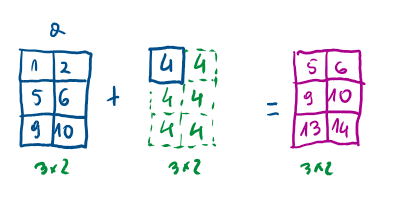
\includegraphics[keepaspectratio]{o3.png}}

Wariant 2 - dwie tablice - ``gdy jedna z tablic może być rozszerzona''
(oba wymiary są równe lub jeden z nich jest równy 1)

\begin{Shaded}
\begin{Highlighting}[]
\ImportTok{import}\NormalTok{ numpy }\ImportTok{as}\NormalTok{ np}

\NormalTok{a }\OperatorTok{=}\NormalTok{ np.array([[}\DecValTok{1}\NormalTok{, }\DecValTok{2}\NormalTok{], [}\DecValTok{5}\NormalTok{, }\DecValTok{6}\NormalTok{]])}
\NormalTok{b }\OperatorTok{=}\NormalTok{ np.array([}\DecValTok{9}\NormalTok{, }\DecValTok{2}\NormalTok{])}
\NormalTok{r1 }\OperatorTok{=}\NormalTok{ a }\OperatorTok{+}\NormalTok{ b}
\BuiltInTok{print}\NormalTok{(r1)}
\NormalTok{r2 }\OperatorTok{=}\NormalTok{ a }\OperatorTok{/}\NormalTok{ b}
\BuiltInTok{print}\NormalTok{(r2)}
\NormalTok{c }\OperatorTok{=}\NormalTok{ np.array([[}\DecValTok{4}\NormalTok{], [}\OperatorTok{{-}}\DecValTok{2}\NormalTok{]])}
\NormalTok{r3 }\OperatorTok{=}\NormalTok{ a }\OperatorTok{+}\NormalTok{ c}
\BuiltInTok{print}\NormalTok{(r3)}
\NormalTok{r4 }\OperatorTok{=}\NormalTok{ c }\OperatorTok{/}\NormalTok{ a}
\BuiltInTok{print}\NormalTok{(r4)}
\end{Highlighting}
\end{Shaded}

\begin{verbatim}
[[10  4]
 [14  8]]
[[0.11111111 1.        ]
 [0.55555556 3.        ]]
[[5 6]
 [3 4]]
[[ 4.          2.        ]
 [-0.4        -0.33333333]]
\end{verbatim}

\pandocbounded{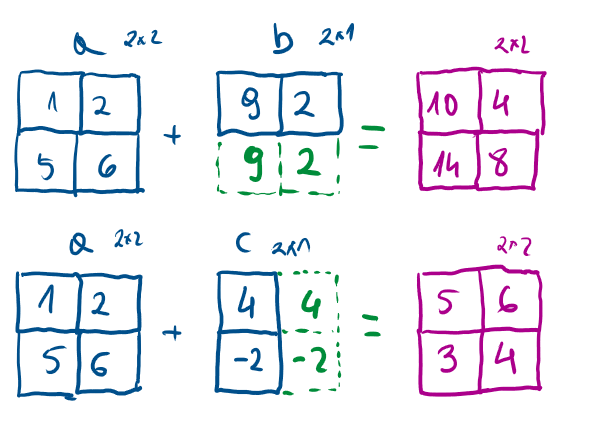
\includegraphics[keepaspectratio]{a4.png}}

Wariant 3 - ``kolumna'' i ``wiersz''

\begin{Shaded}
\begin{Highlighting}[]
\ImportTok{import}\NormalTok{ numpy }\ImportTok{as}\NormalTok{ np}

\NormalTok{a }\OperatorTok{=}\NormalTok{ np.array([[}\DecValTok{5}\NormalTok{, }\DecValTok{2}\NormalTok{, }\OperatorTok{{-}}\DecValTok{3}\NormalTok{]]).T}
\NormalTok{b }\OperatorTok{=}\NormalTok{ np.array([}\DecValTok{3}\NormalTok{, }\OperatorTok{{-}}\DecValTok{2}\NormalTok{, }\DecValTok{1}\NormalTok{, }\DecValTok{2}\NormalTok{, }\DecValTok{4}\NormalTok{])}
\BuiltInTok{print}\NormalTok{(a}\OperatorTok{+}\NormalTok{b)}
\BuiltInTok{print}\NormalTok{(b}\OperatorTok{+}\NormalTok{a)}
\BuiltInTok{print}\NormalTok{(a}\OperatorTok{*}\NormalTok{b)}
\end{Highlighting}
\end{Shaded}

\begin{verbatim}
[[ 8  3  6  7  9]
 [ 5  0  3  4  6]
 [ 0 -5 -2 -1  1]]
[[ 8  3  6  7  9]
 [ 5  0  3  4  6]
 [ 0 -5 -2 -1  1]]
[[ 15 -10   5  10  20]
 [  6  -4   2   4   8]
 [ -9   6  -3  -6 -12]]
\end{verbatim}

\pandocbounded{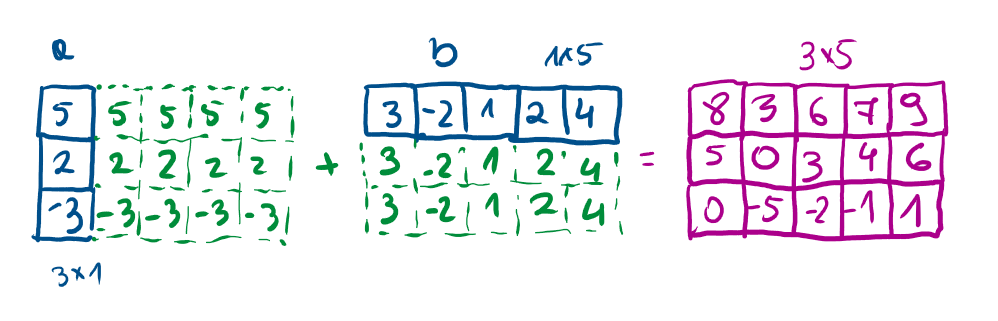
\includegraphics[keepaspectratio]{o5.png}}

\textbf{Ćwiczenia:} (\texttt{ex6.py})

\begin{enumerate}
\def\labelenumi{\arabic{enumi}.}
\item
  Rozważ jednowymiarową tablicę\\
  \[A = \begin{bmatrix}1 & 2 & 3\end{bmatrix}\]\\
  oraz skalar \(k = 10\).\\
  Wykonaj dodawanie, odejmowanie, mnożenie i dzielenie każdego elementu
  tablicy \(A\) przez \(k\) z wykorzystaniem broadcastingu.
\item
  Dla dwóch tablic jednowymiarowych\\
  \[B_1 = \begin{bmatrix}1 & 2 & 3\end{bmatrix}, \quad B_2 = \begin{bmatrix}4 & 5 & 6\end{bmatrix},\]\\
  wykonaj działanie \(B_1 + B_2\), \(B_1 - B_2\), \(B_1 * B_2\) oraz
  \(B_1 / B_2\) używając broadcastingu.
\item
  Mając dwie tablice dwuwymiarowe:\\
  \[C_1 = \begin{bmatrix}1 & 2 \\ 3 & 4\end{bmatrix}, \quad C_2 = \begin{bmatrix}10 & 20 \\ 30 & 40\end{bmatrix},\]\\
  dodaj je i odejmij od siebie, sprawdzając czy broadcasting zajdzie
  automatycznie.
\item
  Rozważ tablicę dwuwymiarową\\
  \[D = \begin{bmatrix}1 & 2 & 3 \\ 4 & 5 & 6\end{bmatrix}\]\\
  oraz wektor\\
  \[v = \begin{bmatrix}10 & 100 & 1000\end{bmatrix}.\]\\
  Wykonaj mnożenie i dzielenie elementowe tablicy \(D\) przez \(v\) z
  wykorzystaniem broadcastingu.
\item
  Dla tablicy\\
  \[E = \begin{bmatrix}2 & 4 & 6 \\ 8 & 10 & 12\end{bmatrix}\]\\
  podnieś każdy element do kwadratu, a następnie podziel przez wektor\\
  \[w = \begin{bmatrix}2 & 2 & 2\end{bmatrix}\]\\
  korzystając z broadcastingu.
\item
  Mając tablicę dwuwymiarową\\
  \[F = \begin{bmatrix}1 & 2 \\ 3 & 4 \\ 5 & 6\end{bmatrix},\]\\
  oraz skalar \(s = 2\), wykonaj \(F * s\), a następnie \(F^{s}\)
  (podnieś każdy element do potęgi \(s\)) z zastosowaniem broadcastingu.
\item
  Rozważ tablicę\\
  \[G = \begin{bmatrix}10 & 20 & 30\end{bmatrix}\]\\
  oraz kolumnową tablicę dwuwymiarową\\
  \[h = \begin{bmatrix}1 \\ 2 \\ 3\end{bmatrix}.\] Dodaj do \(h\)
  tablicę \(G\) i zaobserwuj wynik broadcastingu.
\item
  Mając dwie tablice dwuwymiarowe o różnych wymiarach:\\
  \[H_1 = \begin{bmatrix}1 & 2 & 3\end{bmatrix}, \quad H_2 = \begin{bmatrix}10 \\ 20 \\ 30\end{bmatrix},\]\\
  spróbuj je dodać i pomnożyć przez siebie, korzystając z broadcastingu.
\item
  Rozważ tablicę dwuwymiarową\\
  \[J = \begin{bmatrix}1 & 2 & 3 \\ 4 & 5 & 6\end{bmatrix}\]\\
  oraz skalar \(m = 5\).\\
  Wykonaj kombinację działań: najpierw pomnóż \(J\) przez \(m\),
  następnie odejmij \(m\), a na końcu podziel wynik przez \(m\) --
  wszystko z wykorzystaniem broadcastingu.
\end{enumerate}

\chapter{Funkcje uniwersalne (ufunc)}\label{funkcje-uniwersalne-ufunc}

Funkcje uniwersalne (tzw. \emph{ufunc}) to jedne z najważniejszych
narzędzi w NumPy. Są to funkcje działające element-po-elemencie na
tablicach, często implementowane w C, co zapewnia wysoką wydajność
obliczeń. Dzięki \emph{ufuncs} można w prosty i czytelny sposób
wykonywać operacje arytmetyczne, trygonometryczne, statystyczne czy
logiczne na całych tablicach bez konieczności pisania pętli w Pythonie.

\section{Podstawowe operacje
arytmetyczne}\label{podstawowe-operacje-arytmetyczne}

NumPy automatycznie przekształca operatory matematyczne w odpowiednie
\emph{ufunc}.\\
Na przykład:

\begin{itemize}
\tightlist
\item
  \texttt{+} odpowiada \texttt{np.add}
\item
  \texttt{-} odpowiada \texttt{np.subtract}
\item
  \texttt{*} odpowiada \texttt{np.multiply}
\item
  \texttt{/} odpowiada \texttt{np.divide}
\item
  \texttt{**} odpowiada \texttt{np.power}
\end{itemize}

Przykład:

\begin{Shaded}
\begin{Highlighting}[]
\ImportTok{import}\NormalTok{ numpy }\ImportTok{as}\NormalTok{ np}

\NormalTok{A }\OperatorTok{=}\NormalTok{ np.array([}\DecValTok{1}\NormalTok{, }\DecValTok{2}\NormalTok{, }\DecValTok{3}\NormalTok{, }\DecValTok{4}\NormalTok{])}
\NormalTok{B }\OperatorTok{=}\NormalTok{ np.array([}\DecValTok{10}\NormalTok{, }\DecValTok{20}\NormalTok{, }\DecValTok{30}\NormalTok{, }\DecValTok{40}\NormalTok{])}

\CommentTok{\# Operacje element{-}po{-}elemencie}
\NormalTok{sum\_tab }\OperatorTok{=}\NormalTok{ np.add(A, B)       }\CommentTok{\# to samo co A + B}
\NormalTok{diff\_tab }\OperatorTok{=}\NormalTok{ np.subtract(B, A) }\CommentTok{\# to samo co B {-} A}
\NormalTok{mul\_tab }\OperatorTok{=}\NormalTok{ np.multiply(A, }\DecValTok{2}\NormalTok{)  }\CommentTok{\# to samo co A * 2}
\NormalTok{pow\_tab }\OperatorTok{=}\NormalTok{ np.power(A, }\DecValTok{3}\NormalTok{)     }\CommentTok{\# to samo co A ** 3}

\BuiltInTok{print}\NormalTok{(}\StringTok{"Suma:"}\NormalTok{, sum\_tab)}
\BuiltInTok{print}\NormalTok{(}\StringTok{"Różnica:"}\NormalTok{, diff\_tab)}
\BuiltInTok{print}\NormalTok{(}\StringTok{"Mnożenie przez 2:"}\NormalTok{, mul\_tab)}
\BuiltInTok{print}\NormalTok{(}\StringTok{"Potęgowanie:"}\NormalTok{, pow\_tab)}
\end{Highlighting}
\end{Shaded}

\begin{verbatim}
Suma: [11 22 33 44]
Różnica: [ 9 18 27 36]
Mnożenie przez 2: [2 4 6 8]
Potęgowanie: [ 1  8 27 64]
\end{verbatim}

\section{Funkcje trygonometryczne i
pochodne}\label{funkcje-trygonometryczne-i-pochodne}

NumPy oferuje bogaty zestaw funkcji trygonometrycznych:

\begin{itemize}
\tightlist
\item
  \texttt{np.sin}, \texttt{np.cos}, \texttt{np.tan} -- funkcje
  podstawowe,
\item
  \texttt{np.arcsin}, \texttt{np.arccos}, \texttt{np.arctan} -- odwrotne
  funkcje trygonometryczne,
\item
  \texttt{np.sinh}, \texttt{np.cosh}, \texttt{np.tanh} -- funkcje
  hiperboliczne.
\end{itemize}

Przykład:

\begin{Shaded}
\begin{Highlighting}[]
\ImportTok{import}\NormalTok{ numpy }\ImportTok{as}\NormalTok{ np}

\NormalTok{x }\OperatorTok{=}\NormalTok{ np.linspace(}\DecValTok{0}\NormalTok{, np.pi, }\DecValTok{5}\NormalTok{) }\CommentTok{\# tablica [0, π/4, π/2, 3π/4, π]}
\NormalTok{sin\_values }\OperatorTok{=}\NormalTok{ np.sin(x)}
\NormalTok{cos\_values }\OperatorTok{=}\NormalTok{ np.cos(x)}

\BuiltInTok{print}\NormalTok{(}\StringTok{"Wartości sin(x):"}\NormalTok{, sin\_values)}
\BuiltInTok{print}\NormalTok{(}\StringTok{"Wartości cos(x):"}\NormalTok{, cos\_values)}
\end{Highlighting}
\end{Shaded}

\begin{verbatim}
Wartości sin(x): [0.00000000e+00 7.07106781e-01 1.00000000e+00 7.07106781e-01
 1.22464680e-16]
Wartości cos(x): [ 1.00000000e+00  7.07106781e-01  6.12323400e-17 -7.07106781e-01
 -1.00000000e+00]
\end{verbatim}

\section{Funkcje wykładnicze i
logarytmiczne}\label{funkcje-wykux142adnicze-i-logarytmiczne}

\begin{itemize}
\tightlist
\item
  \texttt{np.exp} -- eksponenta,
\item
  \texttt{np.log} -- logarytm naturalny,
\item
  \texttt{np.log10} -- logarytm dziesiętny.
\end{itemize}

Przykład:

\begin{Shaded}
\begin{Highlighting}[]
\ImportTok{import}\NormalTok{ numpy }\ImportTok{as}\NormalTok{ np}

\NormalTok{A }\OperatorTok{=}\NormalTok{ np.array([}\DecValTok{1}\NormalTok{, np.e, np.e}\OperatorTok{**}\DecValTok{2}\NormalTok{])}
\BuiltInTok{print}\NormalTok{(}\StringTok{"A:"}\NormalTok{, A)}
\BuiltInTok{print}\NormalTok{(}\StringTok{"log(A):"}\NormalTok{, np.log(A))}
\BuiltInTok{print}\NormalTok{(}\StringTok{"exp(A):"}\NormalTok{, np.exp([}\DecValTok{0}\NormalTok{, }\DecValTok{1}\NormalTok{, }\DecValTok{2}\NormalTok{]))  }\CommentTok{\# exp(0)=1, exp(1)=e, exp(2)=e\^{}2}
\end{Highlighting}
\end{Shaded}

\begin{verbatim}
A: [1.         2.71828183 7.3890561 ]
log(A): [0. 1. 2.]
exp(A): [1.         2.71828183 7.3890561 ]
\end{verbatim}

\section{Funkcje zaokrąglające i wartości
bezwzględne}\label{funkcje-zaokrux105glajux105ce-i-wartoux15bci-bezwzglux119dne}

\begin{itemize}
\tightlist
\item
  \texttt{np.round} -- zaokrągla do najbliższej liczby,
\item
  \texttt{np.floor} -- podłoga,
\item
  \texttt{np.ceil} -- sufit,
\item
  \texttt{np.trunc} -- obcięcie do części całkowitej,
\item
  \texttt{np.abs} -- wartość bezwzględna.
\end{itemize}

Przykład:

\begin{Shaded}
\begin{Highlighting}[]
\ImportTok{import}\NormalTok{ numpy }\ImportTok{as}\NormalTok{ np}

\NormalTok{B }\OperatorTok{=}\NormalTok{ np.array([}\FloatTok{1.7}\NormalTok{, }\OperatorTok{{-}}\FloatTok{2.5}\NormalTok{, }\FloatTok{3.5}\NormalTok{, }\OperatorTok{{-}}\FloatTok{4.1}\NormalTok{])}
\BuiltInTok{print}\NormalTok{(}\StringTok{"B:"}\NormalTok{, B)}
\BuiltInTok{print}\NormalTok{(}\StringTok{"floor(B):"}\NormalTok{, np.floor(B))}
\BuiltInTok{print}\NormalTok{(}\StringTok{"ceil(B):"}\NormalTok{, np.ceil(B))}
\BuiltInTok{print}\NormalTok{(}\StringTok{"abs(B):"}\NormalTok{, np.}\BuiltInTok{abs}\NormalTok{(B))}
\end{Highlighting}
\end{Shaded}

\begin{verbatim}
B: [ 1.7 -2.5  3.5 -4.1]
floor(B): [ 1. -3.  3. -5.]
ceil(B): [ 2. -2.  4. -4.]
abs(B): [1.7 2.5 3.5 4.1]
\end{verbatim}

\section{Funkcje statystyczne i
agregujące}\label{funkcje-statystyczne-i-agregujux105ce}

Choć wiele funkcji statystycznych dostępnych jest jako metody tablic
(np. \texttt{A.mean()}, \texttt{A.std()}), istnieją też ufuncs
działające element-po-elemencie lub akceptujące parametry osi:

\begin{itemize}
\tightlist
\item
  \texttt{np.minimum}, \texttt{np.maximum} -- zwracają minimum/maksimum
  element-po-elemencie z dwóch tablic,
\item
  \texttt{np.fmin}, \texttt{np.fmax} -- podobne do wyżej wymienionych,
  ale ignorują wartości NaN,
\item
  \texttt{np.sqrt} -- pierwiastek kwadratowy,
\item
  \texttt{np.square} -- podniesienie do kwadratu.
\end{itemize}

Przykład:

\begin{Shaded}
\begin{Highlighting}[]
\ImportTok{import}\NormalTok{ numpy }\ImportTok{as}\NormalTok{ np}

\NormalTok{C1 }\OperatorTok{=}\NormalTok{ np.array([}\DecValTok{1}\NormalTok{, }\DecValTok{4}\NormalTok{, }\DecValTok{9}\NormalTok{, }\DecValTok{16}\NormalTok{])}
\NormalTok{C2 }\OperatorTok{=}\NormalTok{ np.array([}\DecValTok{2}\NormalTok{, }\DecValTok{2}\NormalTok{, }\DecValTok{5}\NormalTok{, }\DecValTok{20}\NormalTok{])}

\BuiltInTok{print}\NormalTok{(}\StringTok{"minimum elementów C1 i C2:"}\NormalTok{, np.minimum(C1, C2))}
\BuiltInTok{print}\NormalTok{(}\StringTok{"maximum elementów C1 i C2:"}\NormalTok{, np.maximum(C1, C2))}
\BuiltInTok{print}\NormalTok{(}\StringTok{"sqrt(C1):"}\NormalTok{, np.sqrt(C1))}
\BuiltInTok{print}\NormalTok{(}\StringTok{"square(C2):"}\NormalTok{, np.square(C2))}
\end{Highlighting}
\end{Shaded}

\begin{verbatim}
minimum elementów C1 i C2: [ 1  2  5 16]
maximum elementów C1 i C2: [ 2  4  9 20]
sqrt(C1): [1. 2. 3. 4.]
square(C2): [  4   4  25 400]
\end{verbatim}

\textbf{Ćwiczenia:} (\texttt{ex7.py})

\begin{enumerate}
\def\labelenumi{\arabic{enumi}.}
\item
  Mając tablicę\\
  \[A = \begin{bmatrix}1 & 4 & 9 & 16\end{bmatrix},\]\\
  zastosuj funkcję uniwersalną, aby obliczyć pierwiastek kwadratowy
  każdego elementu.
\item
  Rozważ jednowymiarową tablicę\\
  \[B = \begin{bmatrix}-1 & -2 & 3 & -4\end{bmatrix},\]\\
  zastosuj funkcję uniwersalną, aby otrzymać wartości bezwzględne
  wszystkich elementów.
\item
  Dla tablicy\\
  \[C = \begin{bmatrix}0 & \pi/2 & \pi & 3\pi/2\end{bmatrix},\]\\
  oblicz wartość funkcji trygonometrycznej dla każdego elementu.
\item
  Mając tablicę\\
  \[D = \begin{bmatrix}1 & e & e^2 \end{bmatrix},\]\\
  zastosuj funkcję uniwersalną, aby obliczyć logarytm naturalny każdego
  elementu.
\item
  Dla tablicy dwuwymiarowej\\
  \[E = \begin{bmatrix}2 & 4 \\ 10 & 20 \end{bmatrix},\]\\
  podziel każdy element przez skalar, a następnie podnieś uzyskane
  wartości do kwadratu.
\item
  Rozważ tablicę\\
  \[F = \begin{bmatrix}1 & 2 & 3\end{bmatrix},\]\\
  podnieś każdy element do trzeciej potęgi, a następnie zastosuj funkcję
  uniwersalną, aby obliczyć eksponentę z otrzymanych wartości.
\item
  Mając tablicę\\
  \[G = \begin{bmatrix}-\pi & -\pi/2 & 0 & \pi/2 & \pi\end{bmatrix},\]\\
  zastosuj odpowiednią funkcję uniwersalną, aby uzyskać cosinus każdego
  elementu.
\item
  Dla tablicy\\
  \[H = \begin{bmatrix}10 & 100 & 1000\end{bmatrix},\]\\
  zastosuj funkcję uniwersalną, aby obliczyć logarytm dziesiętny każdego
  elementu.
\item
  Mając tablicę\\
  \[I = \begin{bmatrix}2 & 8 & 18 & 32\end{bmatrix},\]\\
  przekształć ją, stosując funkcję uniwersalną, tak aby każdy element
  był pierwiastkiem kwadratowym z wartości początkowej, a następnie
  pomnóż wyniki przez 2.
\item
  Rozważ tablicę\\
  \[J = \begin{bmatrix}-1 & -4 & -9 & -16\end{bmatrix},\]\\
  oblicz pierwiastek kwadratowy wartości bezwzględnych elementów tej
  tablicy, wykorzystując po kolei dwie różne funkcje uniwersalne.
\end{enumerate}

\chapter{Operacje na stringach}\label{operacje-na-stringach}

W \texttt{NumPy} poza dobrze znanymi tablicami liczbowymi, istnieje
również zestaw funkcji pozwalających na wektorowe operacje na ciągach
znaków.

\textbf{Ważne:} Poniższe funkcje są zazwyczaj dostępne w module
\texttt{numpy.char}. W dokumentacji znajdują się one w sekcji
\href{https://numpy.org/doc/stable/reference/routines.strings.html}{String
operations}, jednak w tym materiale skupimy się na tym, jak można je
wykorzystywać, zakładając interfejs z modułu \texttt{numpy.strings}.
Jest to analogiczne do korzystania z \texttt{numpy.char}. Jest no nowsze
podejście.

\section{Tworzenie tablic z napisami}\label{tworzenie-tablic-z-napisami}

NumPy pozwala na przechowywanie tekstu w tablicach, np. tak:

\begin{Shaded}
\begin{Highlighting}[]
\ImportTok{import}\NormalTok{ numpy }\ImportTok{as}\NormalTok{ np}

\NormalTok{arr }\OperatorTok{=}\NormalTok{ np.array([}\StringTok{"python"}\NormalTok{, }\StringTok{"NumPy"}\NormalTok{, }\StringTok{"data"}\NormalTok{, }\StringTok{"Science"}\NormalTok{])}
\BuiltInTok{print}\NormalTok{(arr)}
\end{Highlighting}
\end{Shaded}

\begin{verbatim}
['python' 'NumPy' 'data' 'Science']
\end{verbatim}

\begin{center}\rule{0.5\linewidth}{0.5pt}\end{center}

\section{Podstawowe funkcje do modyfikacji
tekstu}\label{podstawowe-funkcje-do-modyfikacji-tekstu}

Poniżej przedstawiono popularne funkcje do modyfikacji tekstu na
tablicach stringów:

\subsection{\texorpdfstring{\texttt{numpy.strings.upper} i
\texttt{numpy.strings.lower}}{numpy.strings.upper i numpy.strings.lower}}\label{numpy.strings.upper-i-numpy.strings.lower}

\begin{itemize}
\tightlist
\item
  \texttt{upper}: Zamiana wszystkich liter na wielkie.
\item
  \texttt{lower}: Zamiana wszystkich liter na małe.
\end{itemize}

\begin{Shaded}
\begin{Highlighting}[]
\ImportTok{import}\NormalTok{ numpy }\ImportTok{as}\NormalTok{ np}

\NormalTok{arr }\OperatorTok{=}\NormalTok{ np.array([}\StringTok{"python"}\NormalTok{, }\StringTok{"NumPy"}\NormalTok{, }\StringTok{"data"}\NormalTok{, }\StringTok{"Science"}\NormalTok{])}

\BuiltInTok{print}\NormalTok{(np.strings.upper(arr))}
\BuiltInTok{print}\NormalTok{(np.strings.lower(arr))}
\end{Highlighting}
\end{Shaded}

\begin{verbatim}
['PYTHON' 'NUMPY' 'DATA' 'SCIENCE']
['python' 'numpy' 'data' 'science']
\end{verbatim}

\subsection{\texorpdfstring{\texttt{numpy.strings.capitalize}}{numpy.strings.capitalize}}\label{numpy.strings.capitalize}

Funkcja \texttt{capitalize} zamienia pierwszą literę wyrazu na wielką, a
pozostałe na małe.

\begin{Shaded}
\begin{Highlighting}[]
\ImportTok{import}\NormalTok{ numpy }\ImportTok{as}\NormalTok{ np}

\NormalTok{arr }\OperatorTok{=}\NormalTok{ np.array([}\StringTok{"python"}\NormalTok{, }\StringTok{"NumPy"}\NormalTok{, }\StringTok{"data"}\NormalTok{, }\StringTok{"Science"}\NormalTok{])}
\BuiltInTok{print}\NormalTok{(np.strings.capitalize(arr))}
\end{Highlighting}
\end{Shaded}

\begin{verbatim}
['Python' 'Numpy' 'Data' 'Science']
\end{verbatim}

\subsection{\texorpdfstring{\texttt{numpy.strings.title}}{numpy.strings.title}}\label{numpy.strings.title}

Funkcja \texttt{title} sprawia, że każda część składowa tekstu (np.
oddzielona spacją) zostaje zamieniona tak, by zaczynała się od wielkiej
litery.

\begin{Shaded}
\begin{Highlighting}[]
\ImportTok{import}\NormalTok{ numpy }\ImportTok{as}\NormalTok{ np}

\NormalTok{arr2 }\OperatorTok{=}\NormalTok{ np.array([}\StringTok{"python data science"}\NormalTok{, }\StringTok{"machine learning"}\NormalTok{, }\StringTok{"deep learning"}\NormalTok{])}
\BuiltInTok{print}\NormalTok{(np.strings.title(arr2))}
\end{Highlighting}
\end{Shaded}

\begin{verbatim}
['Python Data Science' 'Machine Learning' 'Deep Learning']
\end{verbatim}

\begin{center}\rule{0.5\linewidth}{0.5pt}\end{center}

\section{Łączenie i rozdzielanie
tekstów}\label{ux142ux105czenie-i-rozdzielanie-tekstuxf3w}

\subsection{\texorpdfstring{\texttt{numpy.strings.add}}{numpy.strings.add}}\label{numpy.strings.add}

Funkcja \texttt{add} łączy elementy tablic tekstowych, działając
podobnie jak operator \texttt{+} na stringach, ale wektorowo.

\begin{Shaded}
\begin{Highlighting}[]
\ImportTok{import}\NormalTok{ numpy }\ImportTok{as}\NormalTok{ np}

\NormalTok{arr\_a }\OperatorTok{=}\NormalTok{ np.array([}\StringTok{"Hello"}\NormalTok{, }\StringTok{"Data"}\NormalTok{])}
\NormalTok{arr\_b }\OperatorTok{=}\NormalTok{ np.array([}\StringTok{"World"}\NormalTok{, }\StringTok{"Science"}\NormalTok{])}

\BuiltInTok{print}\NormalTok{(np.strings.add(arr\_a, arr\_b))}
\end{Highlighting}
\end{Shaded}

\begin{verbatim}
['HelloWorld' 'DataScience']
\end{verbatim}

\subsection{\texorpdfstring{\texttt{numpy.strings.join}}{numpy.strings.join}}\label{numpy.strings.join}

Funkcja \texttt{join} pozwala na łączenie elementów tablicy przy użyciu
wskazanego separatora.

\begin{Shaded}
\begin{Highlighting}[]
\ImportTok{import}\NormalTok{ numpy }\ImportTok{as}\NormalTok{ np}

\NormalTok{arr3 }\OperatorTok{=}\NormalTok{ np.array([}\StringTok{"python"}\NormalTok{, }\StringTok{"numpy"}\NormalTok{, }\StringTok{"string"}\NormalTok{])}
\BuiltInTok{print}\NormalTok{(np.char.join(}\StringTok{"{-}"}\NormalTok{, arr3))}
\end{Highlighting}
\end{Shaded}

\begin{verbatim}
['p-y-t-h-o-n' 'n-u-m-p-y' 's-t-r-i-n-g']
\end{verbatim}

\begin{quote}
Uwaga: \texttt{join} wektoryzuje operację, traktując każdy element
tablicy jako sekwencję znaków do połączenia separatorem.
\end{quote}

\subsection{\texorpdfstring{\texttt{numpy.strings.split}}{numpy.strings.split}}\label{numpy.strings.split}

Pozwala na rozdzielanie stringów według podanego separatora. Zwraca
tablicę zawierającą listy podłańcuchów.

\begin{Shaded}
\begin{Highlighting}[]
\ImportTok{import}\NormalTok{ numpy }\ImportTok{as}\NormalTok{ np}

\NormalTok{arr4 }\OperatorTok{=}\NormalTok{ np.array([}\StringTok{"python{-}data{-}science"}\NormalTok{, }\StringTok{"machine{-}learning"}\NormalTok{])}
\BuiltInTok{print}\NormalTok{(np.char.split(arr4, sep}\OperatorTok{=}\StringTok{"{-}"}\NormalTok{))}
\end{Highlighting}
\end{Shaded}

\begin{verbatim}
[list(['python', 'data', 'science']) list(['machine', 'learning'])]
\end{verbatim}

\begin{center}\rule{0.5\linewidth}{0.5pt}\end{center}

\section{Wyszukiwanie i zamiana
podciągów}\label{wyszukiwanie-i-zamiana-podciux105guxf3w}

\subsection{\texorpdfstring{\texttt{numpy.strings.find} i
\texttt{numpy.strings.rfind}}{numpy.strings.find i numpy.strings.rfind}}\label{numpy.strings.find-i-numpy.strings.rfind}

\begin{itemize}
\tightlist
\item
  \texttt{find}: Zwraca indeks pierwszego wystąpienia podłańcucha (lub
  -1, jeśli nie znaleziono).
\item
  \texttt{rfind}: Zwraca indeks ostatniego wystąpienia podłańcucha (lub
  -1, jeśli nie znaleziono).
\end{itemize}

\begin{Shaded}
\begin{Highlighting}[]
\ImportTok{import}\NormalTok{ numpy }\ImportTok{as}\NormalTok{ np}

\NormalTok{arr5 }\OperatorTok{=}\NormalTok{ np.array([}\StringTok{"python"}\NormalTok{, }\StringTok{"data"}\NormalTok{, }\StringTok{"numpy"}\NormalTok{])}
\BuiltInTok{print}\NormalTok{(np.strings.find(arr5, }\StringTok{"a"}\NormalTok{))}
\end{Highlighting}
\end{Shaded}

\begin{verbatim}
[-1  1 -1]
\end{verbatim}

\subsection{\texorpdfstring{\texttt{numpy.strings.replace}}{numpy.strings.replace}}\label{numpy.strings.replace}

\texttt{replace} zamienia wszystkie wystąpienia podłańcucha na nowy ciąg
znaków.

\begin{Shaded}
\begin{Highlighting}[]
\ImportTok{import}\NormalTok{ numpy }\ImportTok{as}\NormalTok{ np}

\NormalTok{arr6 }\OperatorTok{=}\NormalTok{ np.array([}\StringTok{"python"}\NormalTok{, }\StringTok{"pydata"}\NormalTok{, }\StringTok{"pypy"}\NormalTok{])}
\BuiltInTok{print}\NormalTok{(np.strings.replace(arr6, }\StringTok{"py"}\NormalTok{, }\StringTok{"PY"}\NormalTok{))}
\end{Highlighting}
\end{Shaded}

\begin{verbatim}
['PYthon' 'PYdata' 'PYPY']
\end{verbatim}

\begin{center}\rule{0.5\linewidth}{0.5pt}\end{center}

\section{Usuwanie zbędnych
znaków}\label{usuwanie-zbux119dnych-znakuxf3w}

\subsection{\texorpdfstring{\texttt{numpy.strings.strip},
\texttt{numpy.strings.lstrip} i
\texttt{numpy.strings.rstrip}}{numpy.strings.strip, numpy.strings.lstrip i numpy.strings.rstrip}}\label{numpy.strings.strip-numpy.strings.lstrip-i-numpy.strings.rstrip}

\begin{itemize}
\tightlist
\item
  \texttt{strip}: Usuwa wskazane znaki z początku i końca.
\item
  \texttt{lstrip}: Usuwa wskazane znaki z lewej strony (początku).
\item
  \texttt{rstrip}: Usuwa wskazane znaki z prawej strony (końca).
\end{itemize}

\begin{Shaded}
\begin{Highlighting}[]
\ImportTok{import}\NormalTok{ numpy }\ImportTok{as}\NormalTok{ np}

\NormalTok{arr7 }\OperatorTok{=}\NormalTok{ np.array([}\StringTok{"   python   "}\NormalTok{, }\StringTok{"  numpy  "}\NormalTok{])}
\BuiltInTok{print}\NormalTok{(np.strings.strip(arr7))}
\end{Highlighting}
\end{Shaded}

\begin{verbatim}
['python' 'numpy']
\end{verbatim}

Możemy również podać niestandardowe znaki do usunięcia:

\begin{Shaded}
\begin{Highlighting}[]
\ImportTok{import}\NormalTok{ numpy }\ImportTok{as}\NormalTok{ np}

\NormalTok{arr8 }\OperatorTok{=}\NormalTok{ np.array([}\StringTok{"\#\#\#data\#\#\#"}\NormalTok{, }\StringTok{"***science***"}\NormalTok{])}
\BuiltInTok{print}\NormalTok{(np.strings.strip(arr8, }\StringTok{"\#*"}\NormalTok{))}
\end{Highlighting}
\end{Shaded}

\begin{verbatim}
['data' 'science']
\end{verbatim}

\chapter{\texorpdfstring{Alegbra liniowa w
\texttt{NumPy}}{Alegbra liniowa w NumPy}}\label{alegbra-liniowa-w-numpy}

\section{Iloczyn skalarny (dot
product)}\label{iloczyn-skalarny-dot-product}

Dla dwóch wektorów, \texttt{dot} oblicza ich iloczyn skalarny.

\begin{Shaded}
\begin{Highlighting}[]
\ImportTok{import}\NormalTok{ numpy }\ImportTok{as}\NormalTok{ np}

\CommentTok{\# Iloczyn skalarny dwóch wektorów}
\NormalTok{a }\OperatorTok{=}\NormalTok{ np.array([}\DecValTok{1}\NormalTok{, }\DecValTok{2}\NormalTok{, }\DecValTok{3}\NormalTok{])}
\NormalTok{b }\OperatorTok{=}\NormalTok{ np.array([}\DecValTok{4}\NormalTok{, }\DecValTok{5}\NormalTok{, }\DecValTok{6}\NormalTok{])}
\NormalTok{result }\OperatorTok{=}\NormalTok{ np.dot(a, b)  }\CommentTok{\# 1*4 + 2*5 + 3*6}
\BuiltInTok{print}\NormalTok{(result)  }\CommentTok{\# Wynik: 32}

\CommentTok{\# Alternatywny zapis za pomocą operatora @}
\NormalTok{result }\OperatorTok{=}\NormalTok{ a }\OperatorTok{@}\NormalTok{ b}
\BuiltInTok{print}\NormalTok{(result)  }\CommentTok{\# Wynik: 32}
\end{Highlighting}
\end{Shaded}

\begin{verbatim}
32
32
\end{verbatim}

\section{Mnożenie macierzowe}\label{mnoux17cenie-macierzowe}

Dla macierzy (tablic dwuwymiarowych), \texttt{dot} wykonuje standardowe
mnożenie macierzowe.

\begin{Shaded}
\begin{Highlighting}[]
\ImportTok{import}\NormalTok{ numpy }\ImportTok{as}\NormalTok{ np}
\CommentTok{\# Mnożenie macierzowe}
\NormalTok{A }\OperatorTok{=}\NormalTok{ np.array([[}\DecValTok{1}\NormalTok{, }\DecValTok{2}\NormalTok{], [}\DecValTok{3}\NormalTok{, }\DecValTok{4}\NormalTok{]])}
\NormalTok{B }\OperatorTok{=}\NormalTok{ np.array([[}\DecValTok{5}\NormalTok{, }\DecValTok{6}\NormalTok{], [}\DecValTok{7}\NormalTok{, }\DecValTok{8}\NormalTok{]])}
\NormalTok{C }\OperatorTok{=}\NormalTok{ np.dot(A, B)}
\BuiltInTok{print}\NormalTok{(C)}
\CommentTok{\# Wynik:}
\CommentTok{\# [[19 22]}
\CommentTok{\#  [43 50]]}

\CommentTok{\# To samo za pomocą operatora @}
\NormalTok{C }\OperatorTok{=}\NormalTok{ A }\OperatorTok{@}\NormalTok{ B}
\BuiltInTok{print}\NormalTok{(C)}
\end{Highlighting}
\end{Shaded}

\begin{verbatim}
[[19 22]
 [43 50]]
[[19 22]
 [43 50]]
\end{verbatim}

\section{Mnożenie macierz-wektor}\label{mnoux17cenie-macierz-wektor}

Możemy również mnożyć macierz przez wektor:

\begin{Shaded}
\begin{Highlighting}[]
\ImportTok{import}\NormalTok{ numpy }\ImportTok{as}\NormalTok{ np}
\CommentTok{\# Mnożenie macierz{-}wektor}
\NormalTok{A }\OperatorTok{=}\NormalTok{ np.array([[}\DecValTok{1}\NormalTok{, }\DecValTok{2}\NormalTok{], [}\DecValTok{3}\NormalTok{, }\DecValTok{4}\NormalTok{]])}
\NormalTok{v }\OperatorTok{=}\NormalTok{ np.array([}\DecValTok{5}\NormalTok{, }\DecValTok{6}\NormalTok{])}
\NormalTok{result }\OperatorTok{=}\NormalTok{ np.dot(A, v)}
\BuiltInTok{print}\NormalTok{(result)  }\CommentTok{\# Wynik: [17 39]}
\end{Highlighting}
\end{Shaded}

\begin{verbatim}
[17 39]
\end{verbatim}

\section{Rozwiązywanie układów równań
liniowych}\label{rozwiux105zywanie-ukux142aduxf3w-ruxf3wnaux144-liniowych}

Funkcja \texttt{numpy.linalg.solve} rozwiązuje układy równań liniowych
postaci Ax = b:

\begin{Shaded}
\begin{Highlighting}[]
\ImportTok{import}\NormalTok{ numpy }\ImportTok{as}\NormalTok{ np}
\CommentTok{\# Rozwiązywanie układu równań liniowych}
\NormalTok{A }\OperatorTok{=}\NormalTok{ np.array([[}\DecValTok{3}\NormalTok{, }\DecValTok{1}\NormalTok{], [}\DecValTok{1}\NormalTok{, }\DecValTok{2}\NormalTok{]])}
\NormalTok{b }\OperatorTok{=}\NormalTok{ np.array([}\DecValTok{9}\NormalTok{, }\DecValTok{8}\NormalTok{])}
\NormalTok{x }\OperatorTok{=}\NormalTok{ np.linalg.solve(A, b)}
\BuiltInTok{print}\NormalTok{(x)  }\CommentTok{\# Wynik: [2. 3.]}

\CommentTok{\# Sprawdzenie rozwiązania}
\NormalTok{np.dot(A, x)  }\CommentTok{\# Powinno być równe b}
\end{Highlighting}
\end{Shaded}

\begin{verbatim}
[2. 3.]
\end{verbatim}

\begin{verbatim}
array([9., 8.])
\end{verbatim}

\section{Wyznacznik macierzy}\label{wyznacznik-macierzy}

Funkcja \texttt{numpy.linalg.det} oblicza wyznacznik macierzy:

\begin{Shaded}
\begin{Highlighting}[]
\ImportTok{import}\NormalTok{ numpy }\ImportTok{as}\NormalTok{ np}
\CommentTok{\# Obliczanie wyznacznika}
\NormalTok{A }\OperatorTok{=}\NormalTok{ np.array([[}\DecValTok{1}\NormalTok{, }\DecValTok{2}\NormalTok{], [}\DecValTok{3}\NormalTok{, }\DecValTok{4}\NormalTok{]])}
\NormalTok{det\_A }\OperatorTok{=}\NormalTok{ np.linalg.det(A)}
\BuiltInTok{print}\NormalTok{(det\_A)  }\CommentTok{\# Wynik: {-}2.0}
\end{Highlighting}
\end{Shaded}

\begin{verbatim}
-2.0000000000000004
\end{verbatim}

\section{Wartości i wektory
własne}\label{wartoux15bci-i-wektory-wux142asne}

Funkcja \texttt{numpy.linalg.eig} oblicza wartości i wektory własne
macierzy:

\begin{Shaded}
\begin{Highlighting}[]
\ImportTok{import}\NormalTok{ numpy }\ImportTok{as}\NormalTok{ np}
\CommentTok{\# Obliczanie wartości i wektorów własnych}
\NormalTok{A }\OperatorTok{=}\NormalTok{ np.array([[}\DecValTok{4}\NormalTok{, }\OperatorTok{{-}}\DecValTok{2}\NormalTok{], [}\DecValTok{1}\NormalTok{, }\DecValTok{1}\NormalTok{]])}
\NormalTok{eigenvalues, eigenvectors }\OperatorTok{=}\NormalTok{ np.linalg.eig(A)}
\BuiltInTok{print}\NormalTok{(}\StringTok{"Wartości własne:"}\NormalTok{, eigenvalues)}
\BuiltInTok{print}\NormalTok{(}\StringTok{"Wektory własne:"}\NormalTok{)}
\BuiltInTok{print}\NormalTok{(eigenvectors)}

\CommentTok{\# Sprawdzenie: A * v = lambda * v}
\ControlFlowTok{for}\NormalTok{ i }\KeywordTok{in} \BuiltInTok{range}\NormalTok{(}\BuiltInTok{len}\NormalTok{(eigenvalues)):}
\NormalTok{    lambda\_i }\OperatorTok{=}\NormalTok{ eigenvalues[i]}
\NormalTok{    v\_i }\OperatorTok{=}\NormalTok{ eigenvectors[:, i]}
    \BuiltInTok{print}\NormalTok{(}\SpecialStringTok{f"λ\_}\SpecialCharTok{\{}\NormalTok{i}\SpecialCharTok{\}}\SpecialStringTok{ = }\SpecialCharTok{\{}\NormalTok{lambda\_i}\SpecialCharTok{\}}\SpecialStringTok{"}\NormalTok{)}
    \BuiltInTok{print}\NormalTok{(}\StringTok{"A * v ="}\NormalTok{, np.dot(A, v\_i))}
    \BuiltInTok{print}\NormalTok{(}\StringTok{"λ * v ="}\NormalTok{, lambda\_i }\OperatorTok{*}\NormalTok{ v\_i)}
\end{Highlighting}
\end{Shaded}

\begin{verbatim}
Wartości własne: [3. 2.]
Wektory własne:
[[0.89442719 0.70710678]
 [0.4472136  0.70710678]]
λ_0 = 3.0
A * v = [2.68328157 1.34164079]
λ * v = [2.68328157 1.34164079]
λ_1 = 2.0
A * v = [1.41421356 1.41421356]
λ * v = [1.41421356 1.41421356]
\end{verbatim}

\section{Rozkład wartości osobliwych
(SVD)}\label{rozkux142ad-wartoux15bci-osobliwych-svd}

Rozkład SVD jest potężnym narzędziem w analizie danych:

\begin{Shaded}
\begin{Highlighting}[]
\ImportTok{import}\NormalTok{ numpy }\ImportTok{as}\NormalTok{ np}
\CommentTok{\# Rozkład SVD}
\NormalTok{A }\OperatorTok{=}\NormalTok{ np.array([[}\DecValTok{1}\NormalTok{, }\DecValTok{2}\NormalTok{], [}\DecValTok{3}\NormalTok{, }\DecValTok{4}\NormalTok{], [}\DecValTok{5}\NormalTok{, }\DecValTok{6}\NormalTok{]])}
\NormalTok{U, s, Vh }\OperatorTok{=}\NormalTok{ np.linalg.svd(A)}
\BuiltInTok{print}\NormalTok{(}\StringTok{"Macierz U:"}\NormalTok{)}
\BuiltInTok{print}\NormalTok{(U)}
\BuiltInTok{print}\NormalTok{(}\StringTok{"Wartości osobliwe:"}\NormalTok{, s)}
\BuiltInTok{print}\NormalTok{(}\StringTok{"Macierz V\^{}H:"}\NormalTok{)}
\BuiltInTok{print}\NormalTok{(Vh)}

\CommentTok{\# Rekonstrukcja macierzy A}
\NormalTok{S }\OperatorTok{=}\NormalTok{ np.zeros((A.shape[}\DecValTok{0}\NormalTok{], A.shape[}\DecValTok{1}\NormalTok{]))}
\NormalTok{S[:}\BuiltInTok{len}\NormalTok{(s), :}\BuiltInTok{len}\NormalTok{(s)] }\OperatorTok{=}\NormalTok{ np.diag(s)}
\NormalTok{A\_reconstructed }\OperatorTok{=}\NormalTok{ U }\OperatorTok{@}\NormalTok{ S }\OperatorTok{@}\NormalTok{ Vh}
\BuiltInTok{print}\NormalTok{(}\StringTok{"Rekonstruowana macierz A:"}\NormalTok{)}
\BuiltInTok{print}\NormalTok{(A\_reconstructed)}
\end{Highlighting}
\end{Shaded}

\begin{verbatim}
Macierz U:
[[-0.2298477   0.88346102  0.40824829]
 [-0.52474482  0.24078249 -0.81649658]
 [-0.81964194 -0.40189603  0.40824829]]
Wartości osobliwe: [9.52551809 0.51430058]
Macierz V^H:
[[-0.61962948 -0.78489445]
 [-0.78489445  0.61962948]]
Rekonstruowana macierz A:
[[1. 2.]
 [3. 4.]
 [5. 6.]]
\end{verbatim}

\section{Norma macierzy/wektora}\label{norma-macierzywektora}

NumPy oferuje różne rodzaje norm:

\begin{Shaded}
\begin{Highlighting}[]
\ImportTok{import}\NormalTok{ numpy }\ImportTok{as}\NormalTok{ np}
\CommentTok{\# Różne normy}
\NormalTok{v }\OperatorTok{=}\NormalTok{ np.array([}\DecValTok{3}\NormalTok{, }\DecValTok{4}\NormalTok{])}
\BuiltInTok{print}\NormalTok{(}\StringTok{"Norma L1:"}\NormalTok{, np.linalg.norm(v, }\DecValTok{1}\NormalTok{))  }\CommentTok{\# Norma L1: 7.0}
\BuiltInTok{print}\NormalTok{(}\StringTok{"Norma L2 (Euklidesowa):"}\NormalTok{, np.linalg.norm(v))  }\CommentTok{\# Norma L2: 5.0}
\BuiltInTok{print}\NormalTok{(}\StringTok{"Norma maksimum:"}\NormalTok{, np.linalg.norm(v, np.inf))  }\CommentTok{\# Norma maksimum: 4.0}

\NormalTok{A }\OperatorTok{=}\NormalTok{ np.array([[}\DecValTok{1}\NormalTok{, }\DecValTok{2}\NormalTok{], [}\DecValTok{3}\NormalTok{, }\DecValTok{4}\NormalTok{]])}
\BuiltInTok{print}\NormalTok{(}\StringTok{"Norma macierzowa Frobeniusa:"}\NormalTok{, np.linalg.norm(A, }\StringTok{\textquotesingle{}fro\textquotesingle{}}\NormalTok{))  }\CommentTok{\# Norma Frobeniusa: 5.477...}
\end{Highlighting}
\end{Shaded}

\begin{verbatim}
Norma L1: 7.0
Norma L2 (Euklidesowa): 5.0
Norma maksimum: 4.0
Norma macierzowa Frobeniusa: 5.477225575051661
\end{verbatim}

\section{Macierz odwrotna}\label{macierz-odwrotna}

Funkcja \texttt{numpy.linalg.inv} oblicza macierz odwrotną:

\begin{Shaded}
\begin{Highlighting}[]
\ImportTok{import}\NormalTok{ numpy }\ImportTok{as}\NormalTok{ np}
\CommentTok{\# Macierz odwrotna}
\NormalTok{A }\OperatorTok{=}\NormalTok{ np.array([[}\DecValTok{1}\NormalTok{, }\DecValTok{2}\NormalTok{], [}\DecValTok{3}\NormalTok{, }\DecValTok{4}\NormalTok{]])}
\NormalTok{A\_inv }\OperatorTok{=}\NormalTok{ np.linalg.inv(A)}
\BuiltInTok{print}\NormalTok{(}\StringTok{"Macierz odwrotna:"}\NormalTok{)}
\BuiltInTok{print}\NormalTok{(A\_inv)}

\CommentTok{\# Sprawdzenie: A * A\^{}({-}1) = I}
\BuiltInTok{print}\NormalTok{(}\StringTok{"A * A\^{}({-}1):"}\NormalTok{)}
\BuiltInTok{print}\NormalTok{(np.dot(A, A\_inv))  }\CommentTok{\# Powinno być bliskie macierzy jednostkowej}
\end{Highlighting}
\end{Shaded}

\begin{verbatim}
Macierz odwrotna:
[[-2.   1. ]
 [ 1.5 -0.5]]
A * A^(-1):
[[1.0000000e+00 0.0000000e+00]
 [8.8817842e-16 1.0000000e+00]]
\end{verbatim}

\section{\texorpdfstring{Funkcja \texttt{numpy.inner} - iloczyn
wewnętrzny}{Funkcja numpy.inner - iloczyn wewnętrzny}}\label{funkcja-numpy.inner---iloczyn-wewnux119trzny}

Funkcja \texttt{inner} oblicza iloczyn wewnętrzny dwóch tablic:

\begin{Shaded}
\begin{Highlighting}[]
\ImportTok{import}\NormalTok{ numpy }\ImportTok{as}\NormalTok{ np}
\CommentTok{\# Iloczyn wewnętrzny}
\NormalTok{a }\OperatorTok{=}\NormalTok{ np.array([}\DecValTok{1}\NormalTok{, }\DecValTok{2}\NormalTok{, }\DecValTok{3}\NormalTok{])}
\NormalTok{b }\OperatorTok{=}\NormalTok{ np.array([}\DecValTok{4}\NormalTok{, }\DecValTok{5}\NormalTok{, }\DecValTok{6}\NormalTok{])}
\NormalTok{result }\OperatorTok{=}\NormalTok{ np.inner(a, b)}
\BuiltInTok{print}\NormalTok{(result)  }\CommentTok{\# 1*4 + 2*5 + 3*6 = 32}

\CommentTok{\# Dla tablic 2D}
\NormalTok{A }\OperatorTok{=}\NormalTok{ np.array([[}\DecValTok{1}\NormalTok{, }\DecValTok{2}\NormalTok{], [}\DecValTok{3}\NormalTok{, }\DecValTok{4}\NormalTok{]])}
\NormalTok{B }\OperatorTok{=}\NormalTok{ np.array([[}\DecValTok{5}\NormalTok{, }\DecValTok{6}\NormalTok{], [}\DecValTok{7}\NormalTok{, }\DecValTok{8}\NormalTok{]])}
\NormalTok{result }\OperatorTok{=}\NormalTok{ np.inner(A, B)}
\BuiltInTok{print}\NormalTok{(result)}
\CommentTok{\# Jest to równoważne wykonaniu iloczynu skalarnego wzdłuż ostatniego wymiaru}
\end{Highlighting}
\end{Shaded}

\begin{verbatim}
32
[[17 23]
 [39 53]]
\end{verbatim}

\section{\texorpdfstring{Funkcja \texttt{numpy.outer} - iloczyn
zewnętrzny}{Funkcja numpy.outer - iloczyn zewnętrzny}}\label{funkcja-numpy.outer---iloczyn-zewnux119trzny}

Funkcja \texttt{outer} oblicza iloczyn zewnętrzny dwóch wektorów:

\begin{Shaded}
\begin{Highlighting}[]
\ImportTok{import}\NormalTok{ numpy }\ImportTok{as}\NormalTok{ np}
\CommentTok{\# Iloczyn zewnętrzny}
\NormalTok{a }\OperatorTok{=}\NormalTok{ np.array([}\DecValTok{1}\NormalTok{, }\DecValTok{2}\NormalTok{, }\DecValTok{3}\NormalTok{])}
\NormalTok{b }\OperatorTok{=}\NormalTok{ np.array([}\DecValTok{4}\NormalTok{, }\DecValTok{5}\NormalTok{, }\DecValTok{6}\NormalTok{])}
\NormalTok{result }\OperatorTok{=}\NormalTok{ np.outer(a, b)}
\BuiltInTok{print}\NormalTok{(result)}
\CommentTok{\# Wynik:}
\CommentTok{\# [[ 4  5  6]}
\CommentTok{\#  [ 8 10 12]}
\CommentTok{\#  [12 15 18]]}
\end{Highlighting}
\end{Shaded}

\begin{verbatim}
[[ 4  5  6]
 [ 8 10 12]
 [12 15 18]]
\end{verbatim}

\section{\texorpdfstring{Funkcja \texttt{numpy.matmul} - mnożenie
macierzowe}{Funkcja numpy.matmul - mnożenie macierzowe}}\label{funkcja-numpy.matmul---mnoux17cenie-macierzowe}

Funkcja \texttt{matmul} jest podobna do \texttt{dot}, ale ma nieco inne
zachowanie dla tablic o wymiarach większych niż 2:

\begin{Shaded}
\begin{Highlighting}[]
\ImportTok{import}\NormalTok{ numpy }\ImportTok{as}\NormalTok{ np}
\CommentTok{\# Porównanie dot i matmul}
\NormalTok{a }\OperatorTok{=}\NormalTok{ np.array([[}\DecValTok{1}\NormalTok{, }\DecValTok{2}\NormalTok{], [}\DecValTok{3}\NormalTok{, }\DecValTok{4}\NormalTok{]])}
\NormalTok{b }\OperatorTok{=}\NormalTok{ np.array([[}\DecValTok{5}\NormalTok{, }\DecValTok{6}\NormalTok{], [}\DecValTok{7}\NormalTok{, }\DecValTok{8}\NormalTok{]])}

\NormalTok{dot\_result }\OperatorTok{=}\NormalTok{ np.dot(a, b)}
\NormalTok{matmul\_result }\OperatorTok{=}\NormalTok{ np.matmul(a, b)}

\BuiltInTok{print}\NormalTok{(}\StringTok{"Wynik dot:"}\NormalTok{)}
\BuiltInTok{print}\NormalTok{(dot\_result)}
\BuiltInTok{print}\NormalTok{(}\StringTok{"Wynik matmul:"}\NormalTok{)}
\BuiltInTok{print}\NormalTok{(matmul\_result)}
\CommentTok{\# Dla 2D są identyczne}

\CommentTok{\# Ale dla tablic 3D i wyższych mogą się różnić}
\end{Highlighting}
\end{Shaded}

\begin{verbatim}
Wynik dot:
[[19 22]
 [43 50]]
Wynik matmul:
[[19 22]
 [43 50]]
\end{verbatim}

\chapter{Filtrowanie zaawansowane}\label{filtrowanie-zaawansowane}

\section{\texorpdfstring{Funkcja
\texttt{nonzero()}}{Funkcja nonzero()}}\label{funkcja-nonzero}

Zwraca indeksy elementów niezerowych w tablicy. Wynik jest zwracany jako
krotka tablic, po jednej dla każdego wymiaru tablicy.

\begin{Shaded}
\begin{Highlighting}[]
\ImportTok{import}\NormalTok{ numpy }\ImportTok{as}\NormalTok{ np}

\NormalTok{arr }\OperatorTok{=}\NormalTok{ np.array([[}\DecValTok{3}\NormalTok{, }\DecValTok{0}\NormalTok{, }\DecValTok{0}\NormalTok{], [}\DecValTok{0}\NormalTok{, }\DecValTok{4}\NormalTok{, }\DecValTok{0}\NormalTok{], [}\DecValTok{5}\NormalTok{, }\DecValTok{6}\NormalTok{, }\DecValTok{0}\NormalTok{]])}
\NormalTok{indeksy }\OperatorTok{=}\NormalTok{ np.nonzero(arr)}
\BuiltInTok{print}\NormalTok{(indeksy)  }\CommentTok{\# (array([0, 1, 2, 2]), array([0, 1, 0, 1]))}

\CommentTok{\# Wydobycie wartości niezerowych}
\NormalTok{wartosci }\OperatorTok{=}\NormalTok{ arr[indeksy]}
\BuiltInTok{print}\NormalTok{(wartosci)  }\CommentTok{\# [3 4 5 6]}

\CommentTok{\# Alternatywnie można użyć:}
\NormalTok{indeksy\_i\_wartosci }\OperatorTok{=}\NormalTok{ np.argwhere(arr }\OperatorTok{!=} \DecValTok{0}\NormalTok{)}
\BuiltInTok{print}\NormalTok{(indeksy\_i\_wartosci)  }
\CommentTok{\# [[0 0]}
\CommentTok{\#  [1 1]}
\CommentTok{\#  [2 0]}
\CommentTok{\#  [2 1]]}
\end{Highlighting}
\end{Shaded}

\begin{verbatim}
(array([0, 1, 2, 2]), array([0, 1, 0, 1]))
[3 4 5 6]
[[0 0]
 [1 1]
 [2 0]
 [2 1]]
\end{verbatim}

\section{\texorpdfstring{Funkcja
\texttt{where()}}{Funkcja where()}}\label{funkcja-where}

Zwraca elementy wybrane z \texttt{x} lub \texttt{y} w zależności od
warunku. Jest to warunkowy selektor elementów.

\begin{Shaded}
\begin{Highlighting}[]
\ImportTok{import}\NormalTok{ numpy }\ImportTok{as}\NormalTok{ np}

\CommentTok{\# Zastąp wartości ujemne przez 0}
\NormalTok{arr }\OperatorTok{=}\NormalTok{ np.array([}\DecValTok{1}\NormalTok{, }\OperatorTok{{-}}\DecValTok{2}\NormalTok{, }\DecValTok{3}\NormalTok{, }\OperatorTok{{-}}\DecValTok{4}\NormalTok{, }\DecValTok{5}\NormalTok{])}
\NormalTok{wynik }\OperatorTok{=}\NormalTok{ np.where(arr }\OperatorTok{\textgreater{}} \DecValTok{0}\NormalTok{, arr, }\DecValTok{0}\NormalTok{)}
\BuiltInTok{print}\NormalTok{(wynik)  }\CommentTok{\# [1 0 3 0 5]}

\CommentTok{\# Zastosowanie w tablicy 2D}
\NormalTok{arr\_2d }\OperatorTok{=}\NormalTok{ np.array([[}\DecValTok{1}\NormalTok{, }\OperatorTok{{-}}\DecValTok{2}\NormalTok{, }\DecValTok{3}\NormalTok{], [}\OperatorTok{{-}}\DecValTok{4}\NormalTok{, }\DecValTok{5}\NormalTok{, }\OperatorTok{{-}}\DecValTok{6}\NormalTok{]])}
\NormalTok{wynik\_2d }\OperatorTok{=}\NormalTok{ np.where(arr\_2d }\OperatorTok{\textless{}} \DecValTok{0}\NormalTok{, }\OperatorTok{{-}}\DecValTok{1}\NormalTok{, arr\_2d)}
\BuiltInTok{print}\NormalTok{(wynik\_2d)}
\CommentTok{\# [[ 1 {-}1  3]}
\CommentTok{\#  [{-}1  5 {-}1]]}
\end{Highlighting}
\end{Shaded}

\begin{verbatim}
[1 0 3 0 5]
[[ 1 -1  3]
 [-1  5 -1]]
\end{verbatim}

\section{\texorpdfstring{Funkcje \texttt{indices()} i
\texttt{ix\_()}}{Funkcje indices() i ix\_()}}\label{funkcje-indices-i-ix_}

\subsection{\texorpdfstring{\texttt{indices()}}{indices()}}\label{indices}

Tworzy tablicę reprezentującą indeksy siatki.

\begin{Shaded}
\begin{Highlighting}[]
\ImportTok{import}\NormalTok{ numpy }\ImportTok{as}\NormalTok{ np}

\CommentTok{\# Tworzenie siatki indeksów 3x4}
\NormalTok{grid }\OperatorTok{=}\NormalTok{ np.indices((}\DecValTok{3}\NormalTok{, }\DecValTok{4}\NormalTok{))}
\BuiltInTok{print}\NormalTok{(grid.shape)  }\CommentTok{\# (2, 3, 4)}
\BuiltInTok{print}\NormalTok{(grid[}\DecValTok{0}\NormalTok{])  }\CommentTok{\# indeksy wierszy}
\CommentTok{\# [[0 0 0 0]}
\CommentTok{\#  [1 1 1 1]}
\CommentTok{\#  [2 2 2 2]]}
\BuiltInTok{print}\NormalTok{(grid[}\DecValTok{1}\NormalTok{])  }\CommentTok{\# indeksy kolumn}
\CommentTok{\# [[0 1 2 3]}
\CommentTok{\#  [0 1 2 3]}
\CommentTok{\#  [0 1 2 3]]}
\end{Highlighting}
\end{Shaded}

\begin{verbatim}
(2, 3, 4)
[[0 0 0 0]
 [1 1 1 1]
 [2 2 2 2]]
[[0 1 2 3]
 [0 1 2 3]
 [0 1 2 3]]
\end{verbatim}

\subsection{\texorpdfstring{\texttt{ix\_()}}{ix\_()}}\label{ix_}

Konstruuje otwartą siatkę z wielu sekwencji, co jest przydatne do
indeksowania wielowymiarowego.

\begin{Shaded}
\begin{Highlighting}[]
\ImportTok{import}\NormalTok{ numpy }\ImportTok{as}\NormalTok{ np}
\NormalTok{x }\OperatorTok{=}\NormalTok{ np.array([}\DecValTok{0}\NormalTok{, }\DecValTok{1}\NormalTok{, }\DecValTok{2}\NormalTok{])}
\NormalTok{y }\OperatorTok{=}\NormalTok{ np.array([}\DecValTok{3}\NormalTok{, }\DecValTok{4}\NormalTok{, }\DecValTok{5}\NormalTok{, }\DecValTok{6}\NormalTok{])}
\NormalTok{indeksy }\OperatorTok{=}\NormalTok{ np.ix\_(x, y)}

\CommentTok{\# Tworzy indeksy dla wszystkich kombinacji (0,3), (0,4), ..., (2,6)}
\BuiltInTok{print}\NormalTok{(indeksy[}\DecValTok{0}\NormalTok{].shape, indeksy[}\DecValTok{1}\NormalTok{].shape)  }\CommentTok{\# (3, 1) (1, 4)}

\CommentTok{\# Użycie do wybierania podtablicy}
\NormalTok{arr }\OperatorTok{=}\NormalTok{ np.arange(}\DecValTok{16}\NormalTok{).reshape(}\DecValTok{4}\NormalTok{, }\DecValTok{4}\NormalTok{)}
\BuiltInTok{print}\NormalTok{(arr)}
\CommentTok{\# [[ 0  1  2  3]}
\CommentTok{\#  [ 4  5  6  7]}
\CommentTok{\#  [ 8  9 10 11]}
\CommentTok{\#  [12 13 14 15]]}

\NormalTok{podtablica }\OperatorTok{=}\NormalTok{ arr[np.ix\_([}\DecValTok{0}\NormalTok{, }\DecValTok{2}\NormalTok{, }\DecValTok{3}\NormalTok{], [}\DecValTok{0}\NormalTok{, }\DecValTok{2}\NormalTok{])]}
\BuiltInTok{print}\NormalTok{(podtablica)}
\CommentTok{\# [[ 0  2]}
\CommentTok{\#  [ 8 10]}
\CommentTok{\#  [12 14]]}
\end{Highlighting}
\end{Shaded}

\begin{verbatim}
(3, 1) (1, 4)
[[ 0  1  2  3]
 [ 4  5  6  7]
 [ 8  9 10 11]
 [12 13 14 15]]
[[ 0  2]
 [ 8 10]
 [12 14]]
\end{verbatim}

\section{\texorpdfstring{\texttt{ogrid} i operacje na
siatkach}{ogrid i operacje na siatkach}}\label{ogrid-i-operacje-na-siatkach}

\texttt{ogrid} pozwala na tworzenie otwartych siatek, co jest pamięciowo
wydajniejsze niż pełne siatki.

\begin{Shaded}
\begin{Highlighting}[]
\ImportTok{import}\NormalTok{ numpy }\ImportTok{as}\NormalTok{ np}

\CommentTok{\# Siatka punktów w zakresie od {-}2 do 2 z krokiem 0.1}
\NormalTok{x, y }\OperatorTok{=}\NormalTok{ np.ogrid[}\OperatorTok{{-}}\DecValTok{2}\NormalTok{:}\DecValTok{2}\NormalTok{:}\FloatTok{0.1}\NormalTok{, }\OperatorTok{{-}}\DecValTok{2}\NormalTok{:}\DecValTok{2}\NormalTok{:}\FloatTok{0.1}\NormalTok{]}
\NormalTok{maska }\OperatorTok{=}\NormalTok{ x}\OperatorTok{**}\DecValTok{2} \OperatorTok{+}\NormalTok{ y}\OperatorTok{**}\DecValTok{2} \OperatorTok{\textless{}=} \DecValTok{1}  \CommentTok{\# Okrąg o promieniu 1}
\BuiltInTok{print}\NormalTok{(maska.shape)  }\CommentTok{\# (40, 40)}
\end{Highlighting}
\end{Shaded}

\begin{verbatim}
(40, 40)
\end{verbatim}

\section{\texorpdfstring{Funkcje \texttt{ravel\_multi\_index()} i
\texttt{unravel\_index()}}{Funkcje ravel\_multi\_index() i unravel\_index()}}\label{funkcje-ravel_multi_index-i-unravel_index}

Te funkcje konwertują między indeksami wielowymiarowymi a płaskimi.

\begin{Shaded}
\begin{Highlighting}[]
\ImportTok{import}\NormalTok{ numpy }\ImportTok{as}\NormalTok{ np}

\CommentTok{\# Konwersja indeksów wielowymiarowych na płaskie}
\NormalTok{indeksy\_wielo }\OperatorTok{=}\NormalTok{ np.array([[}\DecValTok{0}\NormalTok{, }\DecValTok{0}\NormalTok{], [}\DecValTok{1}\NormalTok{, }\DecValTok{1}\NormalTok{], [}\DecValTok{2}\NormalTok{, }\DecValTok{1}\NormalTok{]])}
\NormalTok{wymiary }\OperatorTok{=}\NormalTok{ (}\DecValTok{3}\NormalTok{, }\DecValTok{3}\NormalTok{)}
\NormalTok{indeksy\_plaskie }\OperatorTok{=}\NormalTok{ np.ravel\_multi\_index(indeksy\_wielo.T, wymiary)}
\BuiltInTok{print}\NormalTok{(indeksy\_plaskie)  }\CommentTok{\# [0 4 7]}

\CommentTok{\# Konwersja indeksów płaskich na wielowymiarowe}
\NormalTok{indeksy\_plaskie }\OperatorTok{=}\NormalTok{ np.array([}\DecValTok{0}\NormalTok{, }\DecValTok{3}\NormalTok{, }\DecValTok{8}\NormalTok{])}
\NormalTok{ksztalt }\OperatorTok{=}\NormalTok{ (}\DecValTok{3}\NormalTok{, }\DecValTok{3}\NormalTok{)}
\NormalTok{indeksy\_wielo }\OperatorTok{=}\NormalTok{ np.unravel\_index(indeksy\_plaskie, ksztalt)}
\BuiltInTok{print}\NormalTok{(indeksy\_wielo)  }\CommentTok{\# (array([0, 1, 2]), array([0, 0, 2]))}
\end{Highlighting}
\end{Shaded}

\begin{verbatim}
[0 4 7]
(array([0, 1, 2]), array([0, 0, 2]))
\end{verbatim}

\section{Indeksy diagonalne}\label{indeksy-diagonalne}

NumPy oferuje wiele funkcji do pracy z diagonalami macierzy.

\begin{Shaded}
\begin{Highlighting}[]
\ImportTok{import}\NormalTok{ numpy }\ImportTok{as}\NormalTok{ np}
\CommentTok{\# Uzyskanie indeksów głównej przekątnej}
\NormalTok{n }\OperatorTok{=} \DecValTok{4}
\NormalTok{indeksy\_diag }\OperatorTok{=}\NormalTok{ np.diag\_indices(n)}
\BuiltInTok{print}\NormalTok{(indeksy\_diag)  }\CommentTok{\# (array([0, 1, 2, 3]), array([0, 1, 2, 3]))}

\CommentTok{\# Zastosowanie do ustawienia głównej przekątnej}
\NormalTok{arr }\OperatorTok{=}\NormalTok{ np.zeros((}\DecValTok{4}\NormalTok{, }\DecValTok{4}\NormalTok{))}
\NormalTok{arr[indeksy\_diag] }\OperatorTok{=} \DecValTok{1}  \CommentTok{\# Ustawienie jedynek na głównej przekątnej}
\BuiltInTok{print}\NormalTok{(arr)}
\CommentTok{\# [[1. 0. 0. 0.]}
\CommentTok{\#  [0. 1. 0. 0.]}
\CommentTok{\#  [0. 0. 1. 0.]}
\CommentTok{\#  [0. 0. 0. 1.]]}

\CommentTok{\# Uzyskanie indeksów z istniejącej tablicy}
\NormalTok{arr2 }\OperatorTok{=}\NormalTok{ np.ones((}\DecValTok{3}\NormalTok{, }\DecValTok{3}\NormalTok{))}
\NormalTok{indeksy\_diag2 }\OperatorTok{=}\NormalTok{ np.diag\_indices\_from(arr2)}
\end{Highlighting}
\end{Shaded}

\begin{verbatim}
(array([0, 1, 2, 3]), array([0, 1, 2, 3]))
[[1. 0. 0. 0.]
 [0. 1. 0. 0.]
 [0. 0. 1. 0.]
 [0. 0. 0. 1.]]
\end{verbatim}

\section{\texorpdfstring{3.1 Funkcja
\texttt{take()}}{3.1 Funkcja take()}}\label{funkcja-take}

Pobiera elementy z tablicy wzdłuż określonej osi na podstawie indeksów.

\begin{Shaded}
\begin{Highlighting}[]
\ImportTok{import}\NormalTok{ numpy }\ImportTok{as}\NormalTok{ np}

\NormalTok{arr }\OperatorTok{=}\NormalTok{ np.array([}\DecValTok{10}\NormalTok{, }\DecValTok{20}\NormalTok{, }\DecValTok{30}\NormalTok{, }\DecValTok{40}\NormalTok{, }\DecValTok{50}\NormalTok{])}
\NormalTok{indeksy }\OperatorTok{=}\NormalTok{ np.array([}\DecValTok{0}\NormalTok{, }\DecValTok{2}\NormalTok{, }\DecValTok{4}\NormalTok{])}
\NormalTok{wynik }\OperatorTok{=}\NormalTok{ np.take(arr, indeksy)}
\BuiltInTok{print}\NormalTok{(wynik)  }\CommentTok{\# [10 30 50]}

\CommentTok{\# W tablicach wielowymiarowych możemy wybrać oś}
\NormalTok{arr\_2d }\OperatorTok{=}\NormalTok{ np.array([[}\DecValTok{1}\NormalTok{, }\DecValTok{2}\NormalTok{, }\DecValTok{3}\NormalTok{], [}\DecValTok{4}\NormalTok{, }\DecValTok{5}\NormalTok{, }\DecValTok{6}\NormalTok{], [}\DecValTok{7}\NormalTok{, }\DecValTok{8}\NormalTok{, }\DecValTok{9}\NormalTok{]])}
\NormalTok{indeksy\_wierszy }\OperatorTok{=}\NormalTok{ np.array([}\DecValTok{0}\NormalTok{, }\DecValTok{2}\NormalTok{])}
\NormalTok{wynik\_2d }\OperatorTok{=}\NormalTok{ np.take(arr\_2d, indeksy\_wierszy, axis}\OperatorTok{=}\DecValTok{0}\NormalTok{)}
\BuiltInTok{print}\NormalTok{(wynik\_2d)}
\CommentTok{\# [[1 2 3]}
\CommentTok{\#  [7 8 9]]}
\end{Highlighting}
\end{Shaded}

\begin{verbatim}
[10 30 50]
[[1 2 3]
 [7 8 9]]
\end{verbatim}

\#\#Funkcja \texttt{take\_along\_axis()}

Pobiera wartości z tablicy poprzez dopasowanie 1D indeksu i fragmentów
danych. Jest bezpieczna dla duplikatów indeksów.

\begin{Shaded}
\begin{Highlighting}[]
\ImportTok{import}\NormalTok{ numpy }\ImportTok{as}\NormalTok{ np}

\NormalTok{arr }\OperatorTok{=}\NormalTok{ np.array([[}\DecValTok{10}\NormalTok{, }\DecValTok{30}\NormalTok{, }\DecValTok{20}\NormalTok{], [}\DecValTok{60}\NormalTok{, }\DecValTok{40}\NormalTok{, }\DecValTok{50}\NormalTok{]])}
\NormalTok{indeksy\_kolejnosc }\OperatorTok{=}\NormalTok{ np.argsort(arr, axis}\OperatorTok{=}\DecValTok{1}\NormalTok{)}
\NormalTok{wynik }\OperatorTok{=}\NormalTok{ np.take\_along\_axis(arr, indeksy\_kolejnosc, axis}\OperatorTok{=}\DecValTok{1}\NormalTok{)}
\BuiltInTok{print}\NormalTok{(wynik)}
\CommentTok{\# [[10 20 30]}
\CommentTok{\#  [40 50 60]]}
\end{Highlighting}
\end{Shaded}

\begin{verbatim}
[[10 20 30]
 [40 50 60]]
\end{verbatim}

\section{\texorpdfstring{Funkcja
\texttt{choose()}}{Funkcja choose()}}\label{funkcja-choose}

Konstruuje tablicę wybierając elementy z listy tablic.

\begin{Shaded}
\begin{Highlighting}[]
\ImportTok{import}\NormalTok{ numpy }\ImportTok{as}\NormalTok{ np}

\NormalTok{opcje }\OperatorTok{=}\NormalTok{ [np.array([}\DecValTok{0}\NormalTok{, }\DecValTok{1}\NormalTok{, }\DecValTok{2}\NormalTok{, }\DecValTok{3}\NormalTok{]),}
\NormalTok{         np.array([}\DecValTok{10}\NormalTok{, }\DecValTok{11}\NormalTok{, }\DecValTok{12}\NormalTok{, }\DecValTok{13}\NormalTok{]),}
\NormalTok{         np.array([}\DecValTok{20}\NormalTok{, }\DecValTok{21}\NormalTok{, }\DecValTok{22}\NormalTok{, }\DecValTok{23}\NormalTok{])]}
\NormalTok{indeksy }\OperatorTok{=}\NormalTok{ np.array([}\DecValTok{0}\NormalTok{, }\DecValTok{2}\NormalTok{, }\DecValTok{1}\NormalTok{, }\DecValTok{0}\NormalTok{])  }\CommentTok{\# Wybiera z której tablicy opcji wziąć element}
\NormalTok{wynik }\OperatorTok{=}\NormalTok{ np.choose(indeksy, opcje)}
\BuiltInTok{print}\NormalTok{(wynik)  }\CommentTok{\# [ 0 22 11  3]}
\end{Highlighting}
\end{Shaded}

\begin{verbatim}
[ 0 21 12  3]
\end{verbatim}

\section{\texorpdfstring{Funkcja
\texttt{compress()}}{Funkcja compress()}}\label{funkcja-compress}

Zwraca wybrane elementy tablicy wzdłuż określonej osi.

\begin{Shaded}
\begin{Highlighting}[]
\ImportTok{import}\NormalTok{ numpy }\ImportTok{as}\NormalTok{ np}
\NormalTok{arr }\OperatorTok{=}\NormalTok{ np.array([[}\DecValTok{1}\NormalTok{, }\DecValTok{2}\NormalTok{, }\DecValTok{3}\NormalTok{], [}\DecValTok{4}\NormalTok{, }\DecValTok{5}\NormalTok{, }\DecValTok{6}\NormalTok{]])}
\NormalTok{maska }\OperatorTok{=}\NormalTok{ np.array([}\VariableTok{True}\NormalTok{, }\VariableTok{False}\NormalTok{, }\VariableTok{True}\NormalTok{])}
\NormalTok{wynik }\OperatorTok{=}\NormalTok{ np.compress(maska, arr, axis}\OperatorTok{=}\DecValTok{1}\NormalTok{)}
\BuiltInTok{print}\NormalTok{(wynik)}
\CommentTok{\# [[1 3]}
\CommentTok{\#  [4 6]]}
\end{Highlighting}
\end{Shaded}

\begin{verbatim}
[[1 3]
 [4 6]]
\end{verbatim}

\section{\texorpdfstring{Funkcje \texttt{diag()} i
\texttt{diagonal()}}{Funkcje diag() i diagonal()}}\label{funkcje-diag-i-diagonal}

Funkcje do pracy z przekątnymi.

\begin{Shaded}
\begin{Highlighting}[]
\ImportTok{import}\NormalTok{ numpy }\ImportTok{as}\NormalTok{ np}

\CommentTok{\# Tworzenie tablicy diagonalnej}
\NormalTok{diag\_arr }\OperatorTok{=}\NormalTok{ np.diag([}\DecValTok{1}\NormalTok{, }\DecValTok{2}\NormalTok{, }\DecValTok{3}\NormalTok{, }\DecValTok{4}\NormalTok{])}
\BuiltInTok{print}\NormalTok{(diag\_arr)}
\CommentTok{\# [[1 0 0 0]}
\CommentTok{\#  [0 2 0 0]}
\CommentTok{\#  [0 0 3 0]}
\CommentTok{\#  [0 0 0 4]]}

\CommentTok{\# Pobieranie diagonali z tablicy}
\NormalTok{arr }\OperatorTok{=}\NormalTok{ np.array([[}\DecValTok{1}\NormalTok{, }\DecValTok{2}\NormalTok{, }\DecValTok{3}\NormalTok{], [}\DecValTok{4}\NormalTok{, }\DecValTok{5}\NormalTok{, }\DecValTok{6}\NormalTok{], [}\DecValTok{7}\NormalTok{, }\DecValTok{8}\NormalTok{, }\DecValTok{9}\NormalTok{]])}
\NormalTok{diag }\OperatorTok{=}\NormalTok{ np.diag(arr)}
\BuiltInTok{print}\NormalTok{(diag)  }\CommentTok{\# [1 5 9]}

\CommentTok{\# Pobieranie przekątnej przesuniętej o 1}
\NormalTok{diag\_offset }\OperatorTok{=}\NormalTok{ np.diagonal(arr, offset}\OperatorTok{=}\DecValTok{1}\NormalTok{)}
\BuiltInTok{print}\NormalTok{(diag\_offset)  }\CommentTok{\# [2 6]}
\end{Highlighting}
\end{Shaded}

\begin{verbatim}
[[1 0 0 0]
 [0 2 0 0]
 [0 0 3 0]
 [0 0 0 4]]
[1 5 9]
[2 6]
\end{verbatim}

\section{\texorpdfstring{Funkcja
\texttt{select()}}{Funkcja select()}}\label{funkcja-select}

Zwraca tablicę zbudowaną z elementów z listy opcji, w zależności od
warunków.

\begin{Shaded}
\begin{Highlighting}[]
\ImportTok{import}\NormalTok{ numpy }\ImportTok{as}\NormalTok{ np}

\NormalTok{warunki }\OperatorTok{=}\NormalTok{ [arr }\OperatorTok{\textless{}} \DecValTok{3}\NormalTok{, arr }\OperatorTok{\textless{}} \DecValTok{6}\NormalTok{, arr }\OperatorTok{\textless{}} \DecValTok{9}\NormalTok{]}
\NormalTok{opcje }\OperatorTok{=}\NormalTok{ [}\DecValTok{100}\NormalTok{, }\DecValTok{200}\NormalTok{, }\DecValTok{300}\NormalTok{]}
\NormalTok{wynik }\OperatorTok{=}\NormalTok{ np.select(warunki, opcje, default}\OperatorTok{=}\DecValTok{400}\NormalTok{)}
\BuiltInTok{print}\NormalTok{(wynik)}
\CommentTok{\# [[100 100 200]}
\CommentTok{\#  [200 200 300]}
\CommentTok{\#  [300 300 400]]}
\end{Highlighting}
\end{Shaded}

\begin{verbatim}
[[100 100 200]
 [200 200 300]
 [300 300 400]]
\end{verbatim}

\section{\texorpdfstring{Funkcja
\texttt{place()}}{Funkcja place()}}\label{funkcja-place}

Zmienia elementy tablicy na podstawie maski i podanych wartości.

\begin{Shaded}
\begin{Highlighting}[]
\ImportTok{import}\NormalTok{ numpy }\ImportTok{as}\NormalTok{ np}

\NormalTok{arr }\OperatorTok{=}\NormalTok{ np.arange(}\DecValTok{5}\NormalTok{)}
\NormalTok{maska }\OperatorTok{=}\NormalTok{ np.array([}\VariableTok{True}\NormalTok{, }\VariableTok{False}\NormalTok{, }\VariableTok{True}\NormalTok{, }\VariableTok{False}\NormalTok{, }\VariableTok{True}\NormalTok{])}
\NormalTok{np.place(arr, maska, [}\OperatorTok{{-}}\DecValTok{1}\NormalTok{, }\OperatorTok{{-}}\DecValTok{2}\NormalTok{, }\OperatorTok{{-}}\DecValTok{3}\NormalTok{])  }\CommentTok{\# Cyklicznie używa wartości [{-}1, {-}2, {-}3]}
\BuiltInTok{print}\NormalTok{(arr)  }\CommentTok{\# [{-}1  1 {-}2  3 {-}3]}
\end{Highlighting}
\end{Shaded}

\begin{verbatim}
[-1  1 -2  3 -3]
\end{verbatim}

\section{\texorpdfstring{Funkcja
\texttt{put()}}{Funkcja put()}}\label{funkcja-put}

Zastępuje określone elementy tablicy podanymi wartościami.

\begin{Shaded}
\begin{Highlighting}[]
\ImportTok{import}\NormalTok{ numpy }\ImportTok{as}\NormalTok{ np}

\NormalTok{arr }\OperatorTok{=}\NormalTok{ np.arange(}\DecValTok{5}\NormalTok{)}
\NormalTok{indeksy }\OperatorTok{=}\NormalTok{ [}\DecValTok{0}\NormalTok{, }\DecValTok{2}\NormalTok{, }\DecValTok{4}\NormalTok{]}
\NormalTok{np.put(arr, indeksy, [}\DecValTok{10}\NormalTok{, }\DecValTok{20}\NormalTok{, }\DecValTok{30}\NormalTok{])}
\BuiltInTok{print}\NormalTok{(arr)  }\CommentTok{\# [10  1 20  3 30]}
\end{Highlighting}
\end{Shaded}

\begin{verbatim}
[10  1 20  3 30]
\end{verbatim}

\section{\texorpdfstring{Funkcja
\texttt{put\_along\_axis()}}{Funkcja put\_along\_axis()}}\label{funkcja-put_along_axis}

Umieszcza wartości w tablicy docelowej, dopasowując 1D indeks i
fragmenty danych wzdłuż określonej osi.

\begin{Shaded}
\begin{Highlighting}[]
\ImportTok{import}\NormalTok{ numpy }\ImportTok{as}\NormalTok{ np}

\NormalTok{arr }\OperatorTok{=}\NormalTok{ np.array([[}\DecValTok{10}\NormalTok{, }\DecValTok{30}\NormalTok{, }\DecValTok{20}\NormalTok{], [}\DecValTok{60}\NormalTok{, }\DecValTok{40}\NormalTok{, }\DecValTok{50}\NormalTok{]])}
\NormalTok{indeksy }\OperatorTok{=}\NormalTok{ np.argmin(arr, axis}\OperatorTok{=}\DecValTok{1}\NormalTok{)}
\NormalTok{indeksy }\OperatorTok{=}\NormalTok{ np.expand\_dims(indeksy, axis}\OperatorTok{=}\DecValTok{1}\NormalTok{)  }\CommentTok{\# Przekształć do kształtu (2, 1)}
\NormalTok{np.put\_along\_axis(arr, indeksy, }\DecValTok{99}\NormalTok{, axis}\OperatorTok{=}\DecValTok{1}\NormalTok{)}
\BuiltInTok{print}\NormalTok{(arr)}
\CommentTok{\# [[99 30 20]}
\CommentTok{\#  [60 40 99]]}
\end{Highlighting}
\end{Shaded}

\begin{verbatim}
[[99 30 20]
 [60 99 50]]
\end{verbatim}

\section{\texorpdfstring{Funkcja
\texttt{putmask()}}{Funkcja putmask()}}\label{funkcja-putmask}

Zmienia elementy tablicy na podstawie warunku i podanych wartości.

\begin{Shaded}
\begin{Highlighting}[]
\ImportTok{import}\NormalTok{ numpy }\ImportTok{as}\NormalTok{ np}

\NormalTok{arr }\OperatorTok{=}\NormalTok{ np.arange(}\DecValTok{5}\NormalTok{)}
\NormalTok{maska }\OperatorTok{=}\NormalTok{ np.array([}\VariableTok{True}\NormalTok{, }\VariableTok{False}\NormalTok{, }\VariableTok{True}\NormalTok{, }\VariableTok{False}\NormalTok{, }\VariableTok{True}\NormalTok{])}
\NormalTok{np.putmask(arr, maska, [}\OperatorTok{{-}}\DecValTok{1}\NormalTok{, }\OperatorTok{{-}}\DecValTok{2}\NormalTok{, }\OperatorTok{{-}}\DecValTok{3}\NormalTok{])  }\CommentTok{\# Cyklicznie używa wartości}
\BuiltInTok{print}\NormalTok{(arr)  }\CommentTok{\# [{-}1  1 {-}2  3 {-}3]}
\end{Highlighting}
\end{Shaded}

\begin{verbatim}
[-1  1 -3  3 -2]
\end{verbatim}

\section{\texorpdfstring{Funkcja
\texttt{fill\_diagonal()}}{Funkcja fill\_diagonal()}}\label{funkcja-fill_diagonal}

Wypełnia główną przekątną tablicy podaną wartością.

\begin{Shaded}
\begin{Highlighting}[]
\ImportTok{import}\NormalTok{ numpy }\ImportTok{as}\NormalTok{ np}

\NormalTok{arr }\OperatorTok{=}\NormalTok{ np.zeros((}\DecValTok{4}\NormalTok{, }\DecValTok{4}\NormalTok{))}
\NormalTok{np.fill\_diagonal(arr, }\DecValTok{5}\NormalTok{)}
\BuiltInTok{print}\NormalTok{(arr)}
\CommentTok{\# [[5. 0. 0. 0.]}
\CommentTok{\#  [0. 5. 0. 0.]}
\CommentTok{\#  [0. 0. 5. 0.]}
\CommentTok{\#  [0. 0. 0. 5.]]}

\NormalTok{arr\_rect }\OperatorTok{=}\NormalTok{ np.zeros((}\DecValTok{4}\NormalTok{, }\DecValTok{4}\NormalTok{, }\DecValTok{4}\NormalTok{))}
\NormalTok{np.fill\_diagonal(arr\_rect, }\DecValTok{9}\NormalTok{)}
\BuiltInTok{print}\NormalTok{(arr\_rect[}\DecValTok{0}\NormalTok{])  }\CommentTok{\# Wypełnia przekątną w każdym "plasterku" 3D tablicy}
\end{Highlighting}
\end{Shaded}

\begin{verbatim}
[[5. 0. 0. 0.]
 [0. 5. 0. 0.]
 [0. 0. 5. 0.]
 [0. 0. 0. 5.]]
[[9. 0. 0. 0.]
 [0. 0. 0. 0.]
 [0. 0. 0. 0.]
 [0. 0. 0. 0.]]
\end{verbatim}

\chapter{Numpy - inne}\label{numpy---inne}

\section{Stałe}\label{staux142e}

\texttt{NumPy} dostarcza kilka znanych stałych matematycznych, które
mogą być przydatne w obliczeniach naukowych i inżynierskich. Wbudowane
stałe takie jak liczba Pi czy podstawa logarytmu naturalnego \texttt{e}
ułatwiają pisanie czytelnego i zwięzłego kodu.

\begin{enumerate}
\def\labelenumi{\arabic{enumi}.}
\tightlist
\item
  \textbf{\texttt{numpy.pi}}

  \begin{itemize}
  \tightlist
  \item
    Reprezentuje liczbę Pi (π) z dużą dokładnością.\\
  \item
    Pi to stosunek obwodu okręgu do jego średnicy.\\
  \item
    W przybliżeniu: \texttt{3.141592653589793}
  \end{itemize}
\item
  \textbf{\texttt{numpy.e}}

  \begin{itemize}
  \tightlist
  \item
    Reprezentuje podstawę logarytmu naturalnego, \texttt{e}.\\
  \item
    \texttt{e} jest wykorzystywane w wielu dziedzinach, takich jak
    analiza matematyczna, probabilistyka, statystyka.\\
  \item
    W przybliżeniu: \texttt{2.718281828459045}
  \end{itemize}
\item
  \textbf{\texttt{numpy.eulergamma}}

  \begin{itemize}
  \tightlist
  \item
    Reprezentuje stałą Eulera-Mascheroniego, zwykle oznaczaną jako γ
    (gamma).
  \item
    Pojawia się w analizie matematycznej, szczególnie w teorii liczb i
    badaniu szeregów harmonicznych.
  \item
    W przybliżeniu: \texttt{0.5772156649015329}
  \end{itemize}
\end{enumerate}

\begin{Shaded}
\begin{Highlighting}[]
\ImportTok{import}\NormalTok{ numpy }\ImportTok{as}\NormalTok{ np}

\CommentTok{\# Promień koła}
\NormalTok{r }\OperatorTok{=} \FloatTok{5.0}

\CommentTok{\# Obwód koła: 2 * π * r}
\NormalTok{obwod }\OperatorTok{=} \DecValTok{2} \OperatorTok{*}\NormalTok{ np.pi }\OperatorTok{*}\NormalTok{ r}
\BuiltInTok{print}\NormalTok{(}\StringTok{"Obwód koła:"}\NormalTok{, obwod)}

\CommentTok{\# Pole koła: π * r\^{}2}
\NormalTok{pole }\OperatorTok{=}\NormalTok{ np.pi }\OperatorTok{*}\NormalTok{ r}\OperatorTok{**}\DecValTok{2}
\BuiltInTok{print}\NormalTok{(}\StringTok{"Pole koła:"}\NormalTok{, pole)}
\end{Highlighting}
\end{Shaded}

\begin{verbatim}
Obwód koła: 31.41592653589793
Pole koła: 78.53981633974483
\end{verbatim}

\begin{Shaded}
\begin{Highlighting}[]
\ImportTok{import}\NormalTok{ numpy }\ImportTok{as}\NormalTok{ np}

\CommentTok{\# Przykładowy punkt x}
\NormalTok{x }\OperatorTok{=} \FloatTok{1.0}

\CommentTok{\# Wartość funkcji e\^{}x}
\NormalTok{exp\_value }\OperatorTok{=}\NormalTok{ np.e}\OperatorTok{**}\NormalTok{x}
\BuiltInTok{print}\NormalTok{(}\StringTok{"e\^{}x dla x=1:"}\NormalTok{, exp\_value)}

\CommentTok{\# Porównanie z funkcją np.exp}
\NormalTok{exp\_compare }\OperatorTok{=}\NormalTok{ np.exp(x)}
\BuiltInTok{print}\NormalTok{(}\StringTok{"Porównanie z np.exp(1):"}\NormalTok{, exp\_compare)}
\end{Highlighting}
\end{Shaded}

\begin{verbatim}
e^x dla x=1: 2.718281828459045
Porównanie z np.exp(1): 2.718281828459045
\end{verbatim}

\section{\texorpdfstring{\texttt{numpy.inf}}{numpy.inf}}\label{numpy.inf}

\begin{itemize}
\tightlist
\item
  \textbf{Opis}: \texttt{np.inf} reprezentuje wartość nieskończoną
  (∞).\\
\item
  Często pojawia się w obliczeniach, gdy wartość danego wyrażenia dąży
  do nieskończoności (np. dzielenie przez zero, pewne limity, itp.).\\
\item
  Przykładowo, \texttt{1.0\ /\ 0.0} zwróci ostrzeżenie i w konsekwencji
  może dać wartość \texttt{inf}.
\end{itemize}

\begin{Shaded}
\begin{Highlighting}[]
\ImportTok{import}\NormalTok{ numpy }\ImportTok{as}\NormalTok{ np}

\CommentTok{\# Zastosowanie w tworzeniu masek logicznych}
\NormalTok{arr }\OperatorTok{=}\NormalTok{ np.array([}\DecValTok{1}\NormalTok{, }\DecValTok{2}\NormalTok{, np.inf, }\DecValTok{4}\NormalTok{, }\DecValTok{5}\NormalTok{])}
\NormalTok{mask }\OperatorTok{=}\NormalTok{ np.isinf(arr)}
\BuiltInTok{print}\NormalTok{(}\StringTok{"Maska elementów o wartości inf:"}\NormalTok{, mask)}
\end{Highlighting}
\end{Shaded}

\begin{verbatim}
Maska elementów o wartości inf: [False False  True False False]
\end{verbatim}

\section{\texorpdfstring{\texttt{numpy.nan}}{numpy.nan}}\label{numpy.nan}

\begin{itemize}
\tightlist
\item
  \textbf{Opis}: \texttt{np.nan} oznacza ``Not a Number'' (NaN), czyli
  wartość nieokreśloną lub niereprezentowalną w systemie liczbowym.\\
\item
  Pojawia się, gdy wynik operacji numerycznej jest nieokreślony, np.
  \texttt{0.0/0.0}, \texttt{inf\ -\ inf} lub przy błędach wczytywania
  danych.\\
\item
  Operacje arytmetyczne z \texttt{nan} zazwyczaj również zwracają
  \texttt{nan}.
\end{itemize}

\begin{Shaded}
\begin{Highlighting}[]
\ImportTok{import}\NormalTok{ numpy }\ImportTok{as}\NormalTok{ np}

\CommentTok{\# Zamiana wartości nan w tablicy}
\NormalTok{data }\OperatorTok{=}\NormalTok{ np.array([}\DecValTok{1}\NormalTok{, }\DecValTok{2}\NormalTok{, np.nan, }\DecValTok{4}\NormalTok{, np.nan])}
\BuiltInTok{print}\NormalTok{(}\StringTok{"Oryginalne dane:"}\NormalTok{, data)}

\CommentTok{\# Wypełnienie wartości nan zerem}
\NormalTok{data\_no\_nan }\OperatorTok{=}\NormalTok{ np.nan\_to\_num(data, nan}\OperatorTok{=}\FloatTok{0.0}\NormalTok{)}
\BuiltInTok{print}\NormalTok{(}\StringTok{"Dane bez nan:"}\NormalTok{, data\_no\_nan)}
\end{Highlighting}
\end{Shaded}

\begin{verbatim}
Oryginalne dane: [ 1.  2. nan  4. nan]
Dane bez nan: [1. 2. 0. 4. 0.]
\end{verbatim}

\section{\texorpdfstring{\texttt{numpy.newaxis}}{numpy.newaxis}}\label{numpy.newaxis}

\begin{itemize}
\tightlist
\item
  \textbf{Opis}: \texttt{np.newaxis} jest specjalną ``stałą''/obiektem
  służącym do zmiany wymiarów tablic przez zwiększenie ich liczby
  wymiarów o 1.
\end{itemize}

\begin{Shaded}
\begin{Highlighting}[]
\ImportTok{import}\NormalTok{ numpy }\ImportTok{as}\NormalTok{ np}

\CommentTok{\# Mamy tablicę 1D}
\NormalTok{vec }\OperatorTok{=}\NormalTok{ np.array([}\DecValTok{1}\NormalTok{, }\DecValTok{2}\NormalTok{, }\DecValTok{3}\NormalTok{, }\DecValTok{4}\NormalTok{])}
\BuiltInTok{print}\NormalTok{(}\StringTok{"Oryginalna tablica:"}\NormalTok{, vec, }\StringTok{"Kształt:"}\NormalTok{, vec.shape)}

\CommentTok{\# Dodajemy nowy wymiar jako wymiar wierszy}
\NormalTok{vec\_as\_col }\OperatorTok{=}\NormalTok{ vec[:, np.newaxis]}
\BuiltInTok{print}\NormalTok{(}\StringTok{"Tablica jako kolumna:}\CharTok{\textbackslash{}n}\StringTok{"}\NormalTok{, vec\_as\_col, }\StringTok{"Kształt:"}\NormalTok{, vec\_as\_col.shape)}

\CommentTok{\# Dodawanie wymiaru na początku}
\NormalTok{vec\_as\_row }\OperatorTok{=}\NormalTok{ vec[np.newaxis, :]}
\BuiltInTok{print}\NormalTok{(}\StringTok{"Tablica jako wiersz:}\CharTok{\textbackslash{}n}\StringTok{"}\NormalTok{, vec\_as\_row, }\StringTok{"Kształt:"}\NormalTok{, vec\_as\_row.shape)}

\CommentTok{\# Kolejny przykład: dodanie wymiaru by z łatwością broadcastować operacje}
\NormalTok{a }\OperatorTok{=}\NormalTok{ np.array([}\DecValTok{10}\NormalTok{, }\DecValTok{20}\NormalTok{, }\DecValTok{30}\NormalTok{])}
\NormalTok{b }\OperatorTok{=}\NormalTok{ np.array([}\DecValTok{1}\NormalTok{, }\DecValTok{2}\NormalTok{])}
\CommentTok{\# Bez nowego wymiaru próba dodania a do b się nie powiedzie, }
\CommentTok{\# bo kształty nie są kompatybilne.}
\CommentTok{\# Z nowym wymiarem a ma kształt (3,1), a b (2,), co pozwala na broadcast}
\NormalTok{sum\_matrix }\OperatorTok{=}\NormalTok{ a[:, np.newaxis] }\OperatorTok{+}\NormalTok{ b}
\BuiltInTok{print}\NormalTok{(}\StringTok{"Operacja z broadcast:}\CharTok{\textbackslash{}n}\StringTok{"}\NormalTok{, sum\_matrix)}
\end{Highlighting}
\end{Shaded}

\begin{verbatim}
Oryginalna tablica: [1 2 3 4] Kształt: (4,)
Tablica jako kolumna:
 [[1]
 [2]
 [3]
 [4]] Kształt: (4, 1)
Tablica jako wiersz:
 [[1 2 3 4]] Kształt: (1, 4)
Operacja z broadcast:
 [[11 12]
 [21 22]
 [31 32]]
\end{verbatim}

\section{Statystyka i agregacja}\label{statystyka-i-agregacja}

\begin{longtable}[]{@{}
  >{\raggedright\arraybackslash}p{(\linewidth - 2\tabcolsep) * \real{0.2558}}
  >{\raggedright\arraybackslash}p{(\linewidth - 2\tabcolsep) * \real{0.7442}}@{}}
\toprule\noalign{}
\begin{minipage}[b]{\linewidth}\raggedright
Funkcja
\end{minipage} & \begin{minipage}[b]{\linewidth}\raggedright
Opis
\end{minipage} \\
\midrule\noalign{}
\endhead
\bottomrule\noalign{}
\endlastfoot
np.mean & Średnia wszystkich wartości w tablicy. \\
np.std & Odchylenie standardowe. \\
np.var & Wariancja. \\
np.sum & Suma wszystkich elementów. \\
np.prod & Iloczyn wszystkich elementów. \\
np.cumsum & Skumulowana suma wszystkich elementów. \\
np.cumprod & Skumulowany iloczyn wszystkich elementów. \\
np.min,np.max & Minimalna/maksymalna wartość w tablicy. \\
np.argmin, np.argmax & Indeks minimalnej/maksymalnej wartości w
tablicy. \\
np.all & Sprawdza czy wszystki elementy są różne od zera. \\
np.any & Sprawdza czy co najmniej jeden z elementów jest różny od
zera. \\
\end{longtable}

\bookmarksetup{startatroot}

\chapter{Etapy eksploracji danych}\label{etapy-eksploracji-danych}

\begin{itemize}
\tightlist
\item
  \textbf{Zbieranie danych}:

  \begin{itemize}
  \tightlist
  \item
    Zebranie danych z różnych źródeł (bazy danych, pliki CSV, API,
    itd.).
  \end{itemize}
\item
  \textbf{Zrozumienie danych}:

  \begin{itemize}
  \tightlist
  \item
    Analiza struktury danych, typów danych i ich znaczenia.
  \item
    Eksploracja wstępnych zależności i trendów.
  \end{itemize}
\item
  \textbf{Czyszczenie danych}:

  \begin{itemize}
  \tightlist
  \item
    Usuwanie braków, błędów i anomalii w danych.
  \item
    Obsługa brakujących wartości i duplikatów.
  \end{itemize}
\item
  \textbf{Transformacja danych}:

  \begin{itemize}
  \tightlist
  \item
    Normalizacja, standaryzacja, kodowanie zmiennych kategorycznych.
  \item
    Tworzenie nowych zmiennych (cech).
  \end{itemize}
\item
  \textbf{Redukcja danych}:

  \begin{itemize}
  \tightlist
  \item
    Selekcja istotnych cech lub zmniejszenie wymiarowości danych (np.
    PCA).
  \end{itemize}
\end{itemize}




\end{document}
